\documentclass{beamer}
% This is the file main.tex
%\usetheme{default}
%\usetheme{Singapore}
%\usetheme{CambridgeUS}
%\usetheme{Frankfurt}
\usecolortheme{seahorse}
%\usecolortheme{rose}
\usefonttheme[onlylarge]{structuresmallcapsserif}
\usefonttheme[onlysmall]{structurebold}
%\setbeamerfont{title}{shape=\itshape,family=\rmfamily}
%\setbeamercolor{title}{fg=red!80!black}
%\setbeamercolor{title}{fg=red!80!black,bg=red!20!white}

% Utilizamos el paquete para usar español
\usepackage[spanish]{babel}
% Utilizamos un paquete para gestionar los acentos
% y las e ¿es
\usepackage[utf8]{inputenc}
% amsmath y amssymb de la American Mathematical 
% Society (fórmulas matemáticas)
\usepackage{amsmath}
\usefonttheme[onlymath]{serif}
%Para que reconozca el entorno verbatim
\usepackage{fancyvrb}
%Definimos nuestra ruta para las imagenes
%Absoluto
%\graphicspath{ {/home/user/images/} }
%Relativo (recomendado) -> según
%https://es.sharelatex.com/learn/Inserting_Images#La_ruta_a_la_carpeta_de_im.C3.A1genes
\graphicspath{ {media/} }


\title[CAE2020]{The new data acquisition system of the LAGO Collaboration based
on the RedPitaya board}
\vspace{1cm}
\subtitle{{\color[rgb]{0.00,0.21,0.47}Congreso Argentino de Electrónica (CAE2020)\\ Buenos Aires - Argentina}}
\author[\texttt{@horacio\_arnaldi}]{Horacio Arnaldi \\ \texttt{{\href{mailto:arnaldi@cab.cnea.gov.ar}{arnaldi@cab.cnea.gov.ar}}}}
%\institute[LabDPR - CAB - IB]{Laboratorio Detección de Partículas y Radiación \\ Centro Atómico Bariloche - Instituto Balseiro}
%%\date{\today}
%\date{}
%\title[Proyecto LAGO]{Las electrónicas actuales de LAGO}
%\subtitle{Escuela Politécnica Nacional \\ Quito, Ecuador}
%\author[\texttt{@horacio\_arnaldi}]{Ing. Horacio Arnaldi \\ \texttt{{\href{mailto:arnaldi@cab.cnea.gov.ar}{arnaldi@cab.cnea.gov.ar}}}}
\institute[LabDPR - CAB - IB]{Laboratorio Detección de Partículas y Radiación \\ Centro Atómico Bariloche - Instituto Balseiro}
%\date{\today}
\date{}

\begin{document}

\begin{frame}
  \hspace*{0.6cm}
  
\includegraphics[height=0.18\textheight]{logos/cnea_logo} \hspace*{1em}
  
\includegraphics[height=0.18\textheight]{logos/balseiro_logo} \hspace*{1em}
  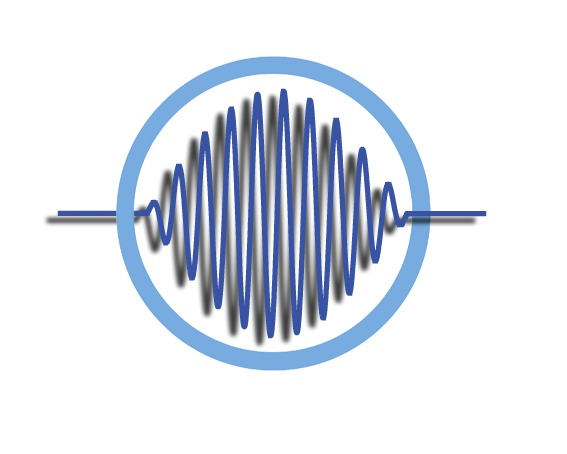
\includegraphics[height=0.18\textheight]{logos/LabDPR_logo} \hspace*{1em}
  
\includegraphics[height=0.18\textheight,width=0.15\textwidth]{logos/lagologo}

  \titlepage

\end{frame}

%\begin{frame}
%  \frametitle{Vista general}
%  \tableofcontents
%%  \tableofcontents[pausesections]
%\end{frame}
%
%

%%------------------------------------------------------------------------------
\section{Las etapas (electrónicas) en LAGO}
%%------------------------------------------------------------------------------
%\begin{frame}
%  \begin{center}
%    \Huge{\color{blue}{Las etapas (electrónicas) en LAGO}}
%  \end{center}
%\end{frame}

\begin{frame}
	\frametitle{¿Qué queremos con la electrónica en LAGO?}
		\begin{block}{}
    	\begin{itemize}
      	\item Obtener la mayor cantidad de información
							posible con el menor costo (pulsos, tiempo
							entre pulsos, amplitudes para frecuencias
							altas de pulsos, etc) 
											\pause
      	\item Sincronización de los diferentes sitios (permite estudiar grandes
							eventos que excitan más de un detector)
											\pause
      	\item Sistema capaz de alimentar/polarizar los fotodetectores
											\pause
      	\item Sistema todo-en-uno
											\pause
        \item Guardar los datos para futuros análisis (off-line data analysis)
              en un lugar centralizado y de fácil acceso para toda la
							Colaboración
											\pause
							\item \alert{Uniformizar el formato de los datos/archivos
											guardados}
											\pause
      	\item Sistema adaptable a otros experimentos (siempre tenemos/queremos
							otros experimentos)

    	\end{itemize}
		\end{block}
\end{frame} 

%\begin{frame}
%	\frametitle{¿Qué queremos con la electrónica en LAGO? (Cont.)}
%		\begin{block}{}
%    	\begin{itemize}
%      	\item Sistema todo-en-uno
%        \item Guardar los datos para futuros análisis (off-line data analysis)
%              en un lugar centralizado y de fácil acceso para toda la
%							Colaboración
%        \item Uniformizar el formato de los datos/archivos guardados
%    	\end{itemize}
%		\end{block}
%\end{frame} 

\begin{frame}
	\frametitle{Los inicios}
				\color[rgb]{0.2,0.2,0.9}{Electrónica dedicada para Auger}
				\begin{columns}
			\begin{column}{0.50\textwidth}
				\begin{block}{}
		    	\begin{itemize}
		      	\item Poco flexible 
		      	\item Documentación/información limitada
		      	\item Número limitado de UBs (Unified Boards)
						\item Comunicación de datos por puerto serie
						\item	Tiempos de adquisición largos
						\item	Poco volumen de almacenamiento
						\item Sin control de línea de base	
		    	\end{itemize}
				\end{block}
			\end{column} 
		 	\begin{column}{0.50\textwidth}
		  	\fbox{\includegraphics[width=\textwidth]{electronica_auger}}
		 \end{column}
		\end{columns}
\end{frame} 

\begin{frame}
	\frametitle{Actualidad: ¿con qué contamos?}
	\begin{columns}
		\begin{column}{0.40\textwidth}
			\begin{block}{}
	    	\begin{itemize}[<+->]
	      	\item Placas de digitalización de 3 y 4 canales
	      	\item GPS para sincronizar los datos de los 
									distintos sitios (Oncore)
					\item Barómetro y sensor de temperatura (HP03)
					\item Placa Nexys2 (FPGA Spartan 3E)
	    	\end{itemize}
			\end{block}
		\end{column} 
	 	\begin{column}{0.55\textwidth}
	  	\only<1-2>{\fbox{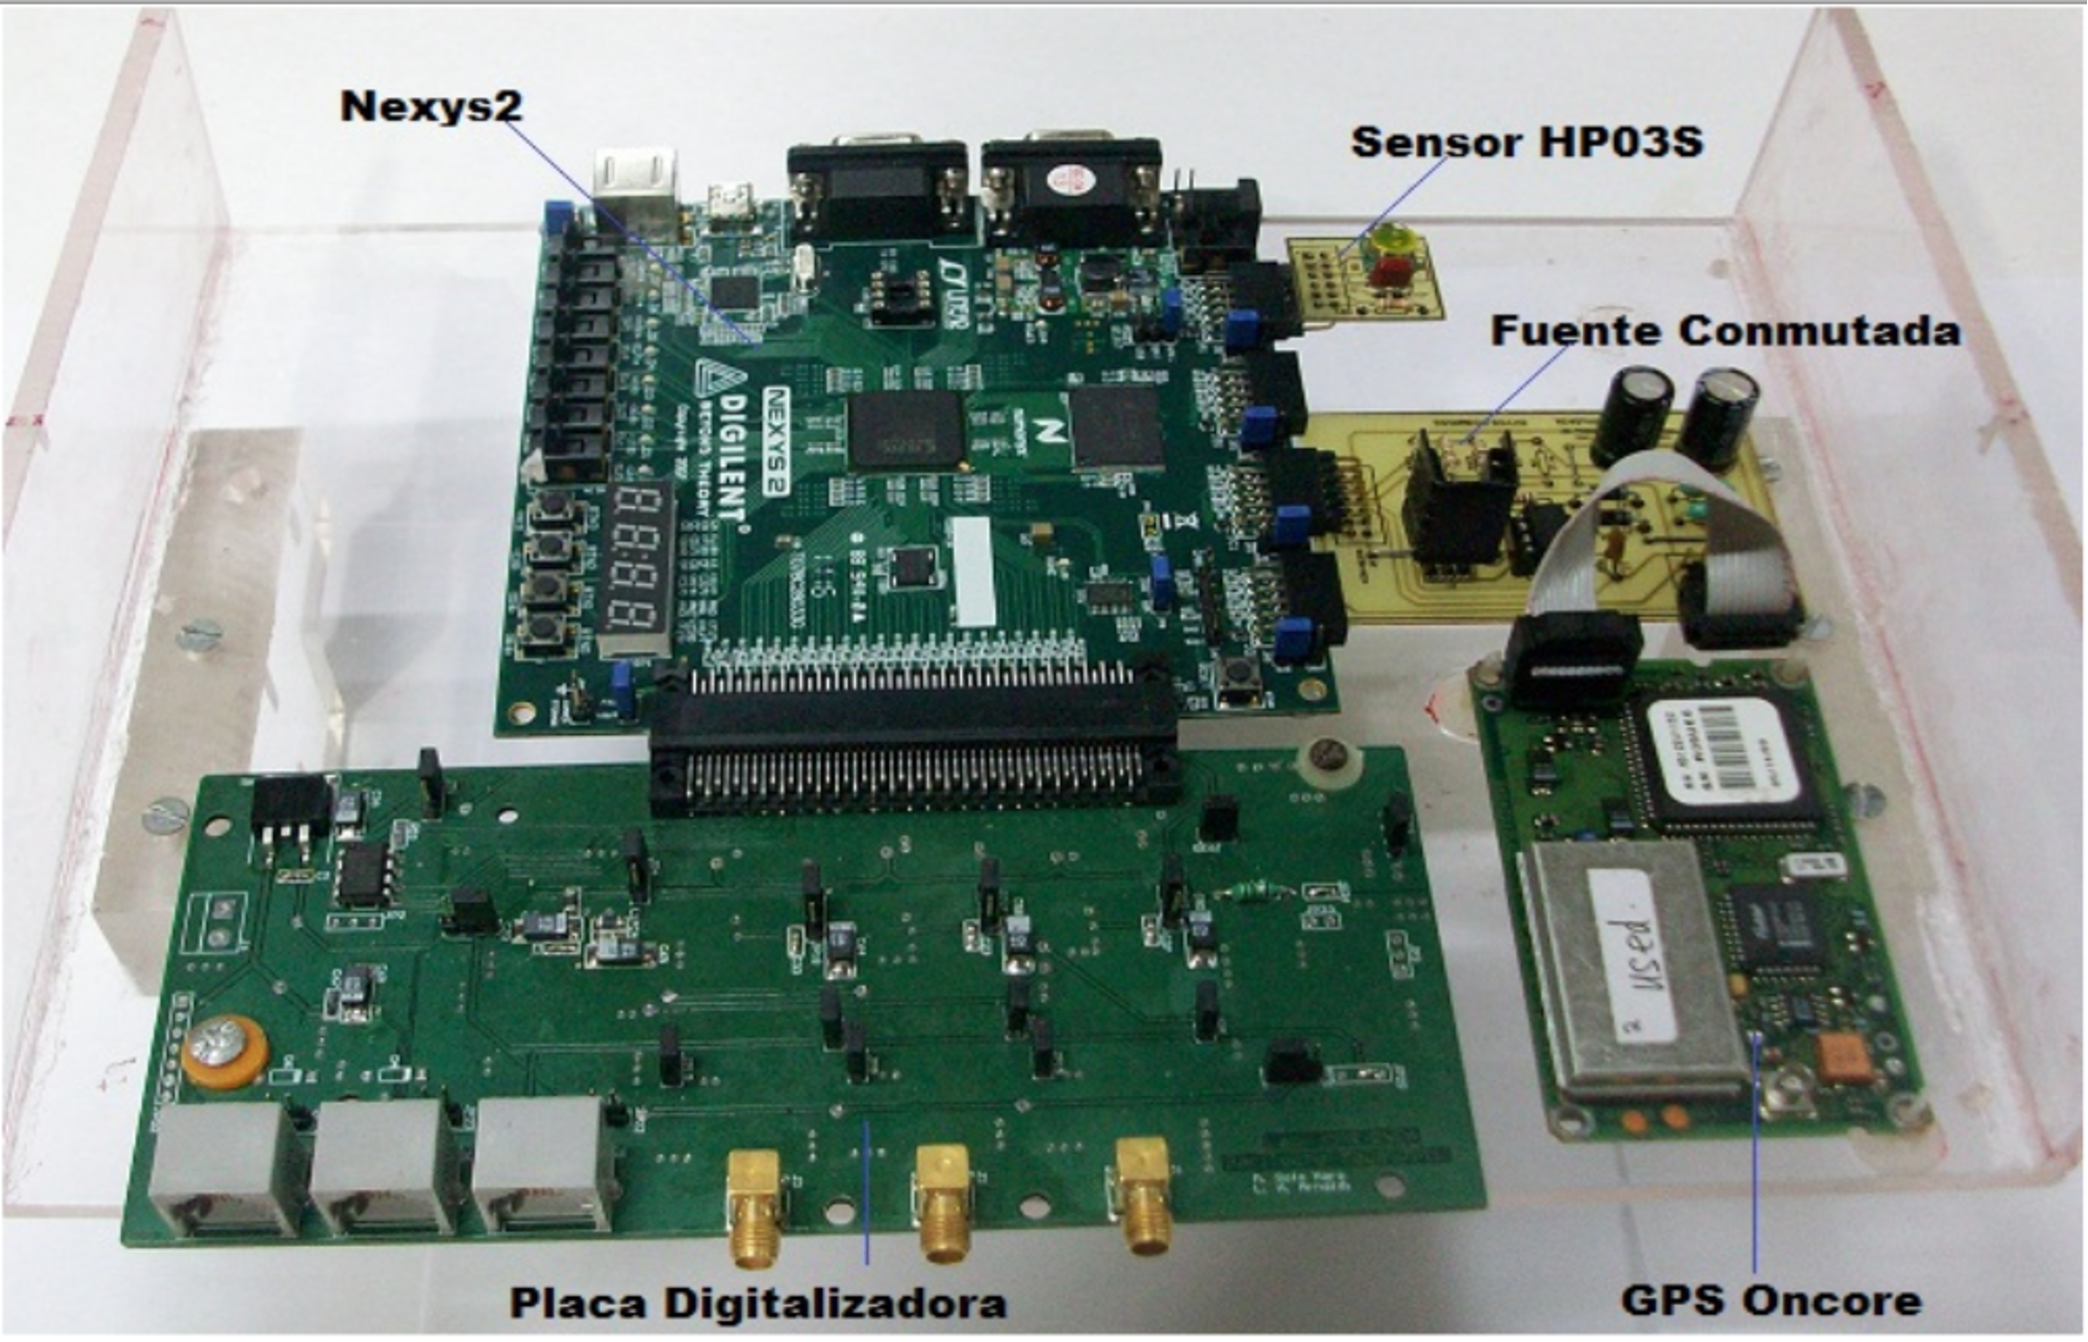
\includegraphics[width=\textwidth]{lago_daq}}}
	  	\only<3-4>{\fbox{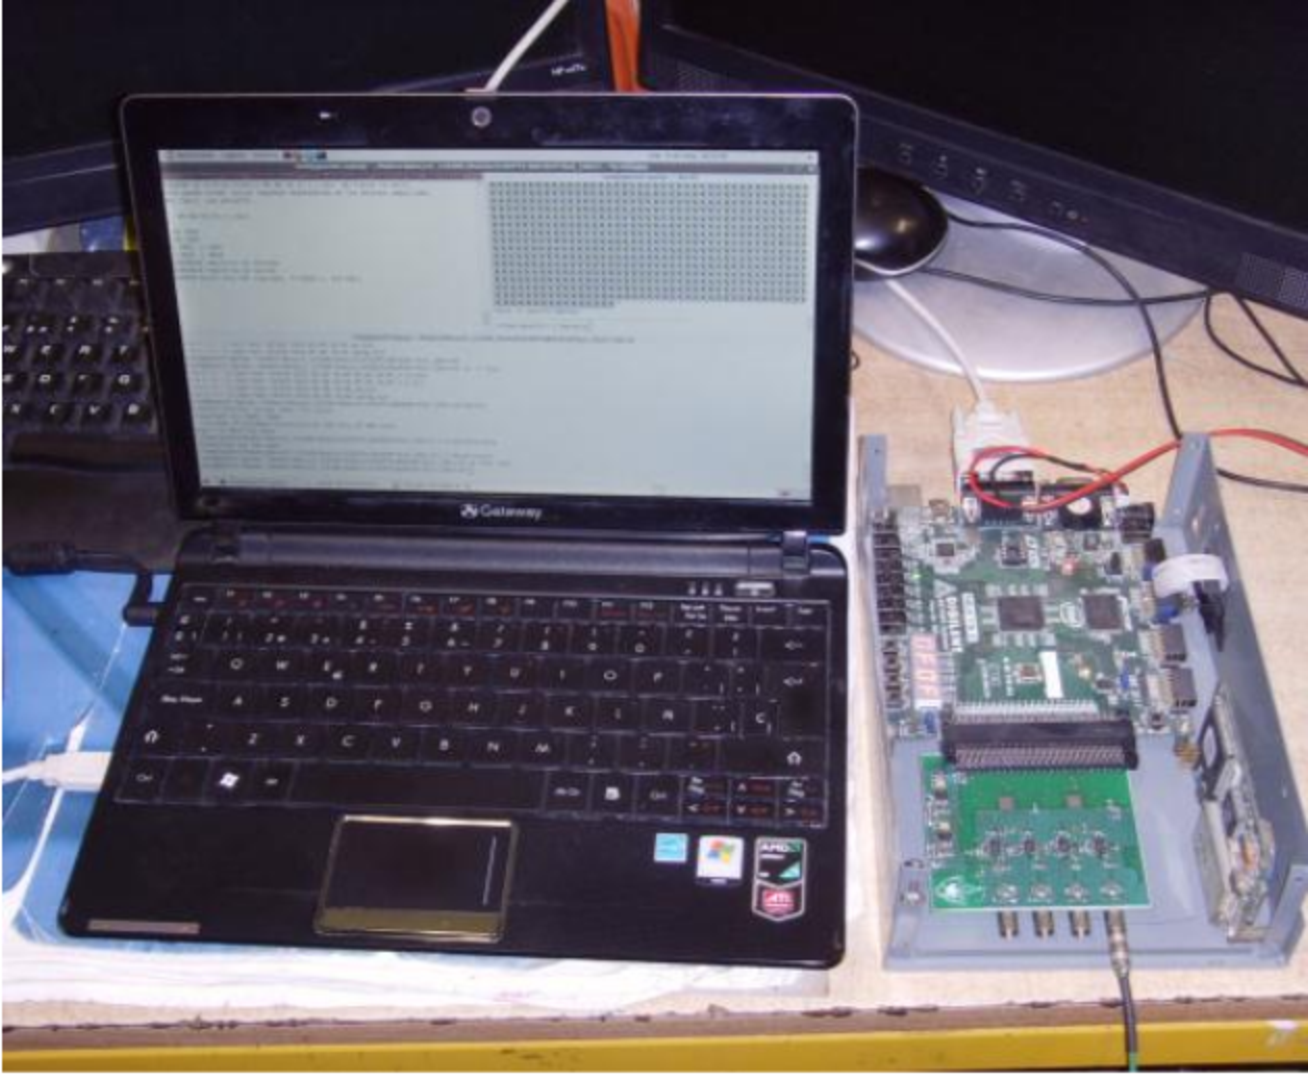
\includegraphics[width=\textwidth]{placa_mx_2}}}
	 \end{column}
	\end{columns}
\end{frame} 

\begin{frame}
	\frametitle{Dificultades actuales}
	\begin{alertblock}{}
		\begin{itemize}
						\item Hasta la aparición del sistema \textcolor{blue}{ACQUA},
										\textcolor{blue}{ANNA}, etc
										(aprox. noviembre de 2015) teníamos (casi) \alert{cada sitio una versión
					diferente del firmware} de la FPGA 
	\item \alert{No todos los sitios pueden estar online con sus datos} (por diversas
					razones, a veces ajenas a la electrónica)
	\item Existencia de dos tipos de electrónicas (\alert{con características muy
					diferentes})
		\item Problemas contínuos con las placas de adquisición (cortos, falsos
					contactos, soldaduras frías, etc) debido a que se ensamblan en casa
		\end{itemize}
	\end{alertblock}
\end{frame} 

\begin{frame}
	\frametitle{Dificultades actuales}
	\begin{alertblock}{}
		\begin{itemize}
		\item ...todo tiene un final, todo termina...
		\item Los GPS Oncore están dejando de funcionar en casi todos los sitios y
						nosotros tenemos la electrónica dedicada a ese GPS particular (\alert{que ya no se
										fabrica más}, además)
		\item Sensores de PyT (HP03) difíciles de conseguir hoy en día
		\item Las placas Nexys2 \alert{¡dejaron de fabricarse!} y constituyen el
					corazón de lo que tenemos actualmente
		\end{itemize}
	\end{alertblock}
\end{frame} 

\begin{frame}
	\frametitle{¿Cuál es la opción?}
	\begin{columns}
		\begin{column}{0.60\textwidth}
			\begin{block}{}
	    	\begin{itemize} %[<+->]
								\item RedPitaya: 2 canales $\sim 62\,\text{MHz}$ (adquisición, 125\,MSPS)
								\item \alert{Linux embebido}
	      	\item Capacidad de conexión y envío de datos a puntos remotos
	      	\item Se pueden conectar los sensores que necesitemos 
					\item Mucha \alert{flexibilidad} (¡justo lo que queremos!)
	    	\end{itemize}
			\end{block}
		\end{column} 
	 	\begin{column}{0.4\textwidth}
	  	\fbox{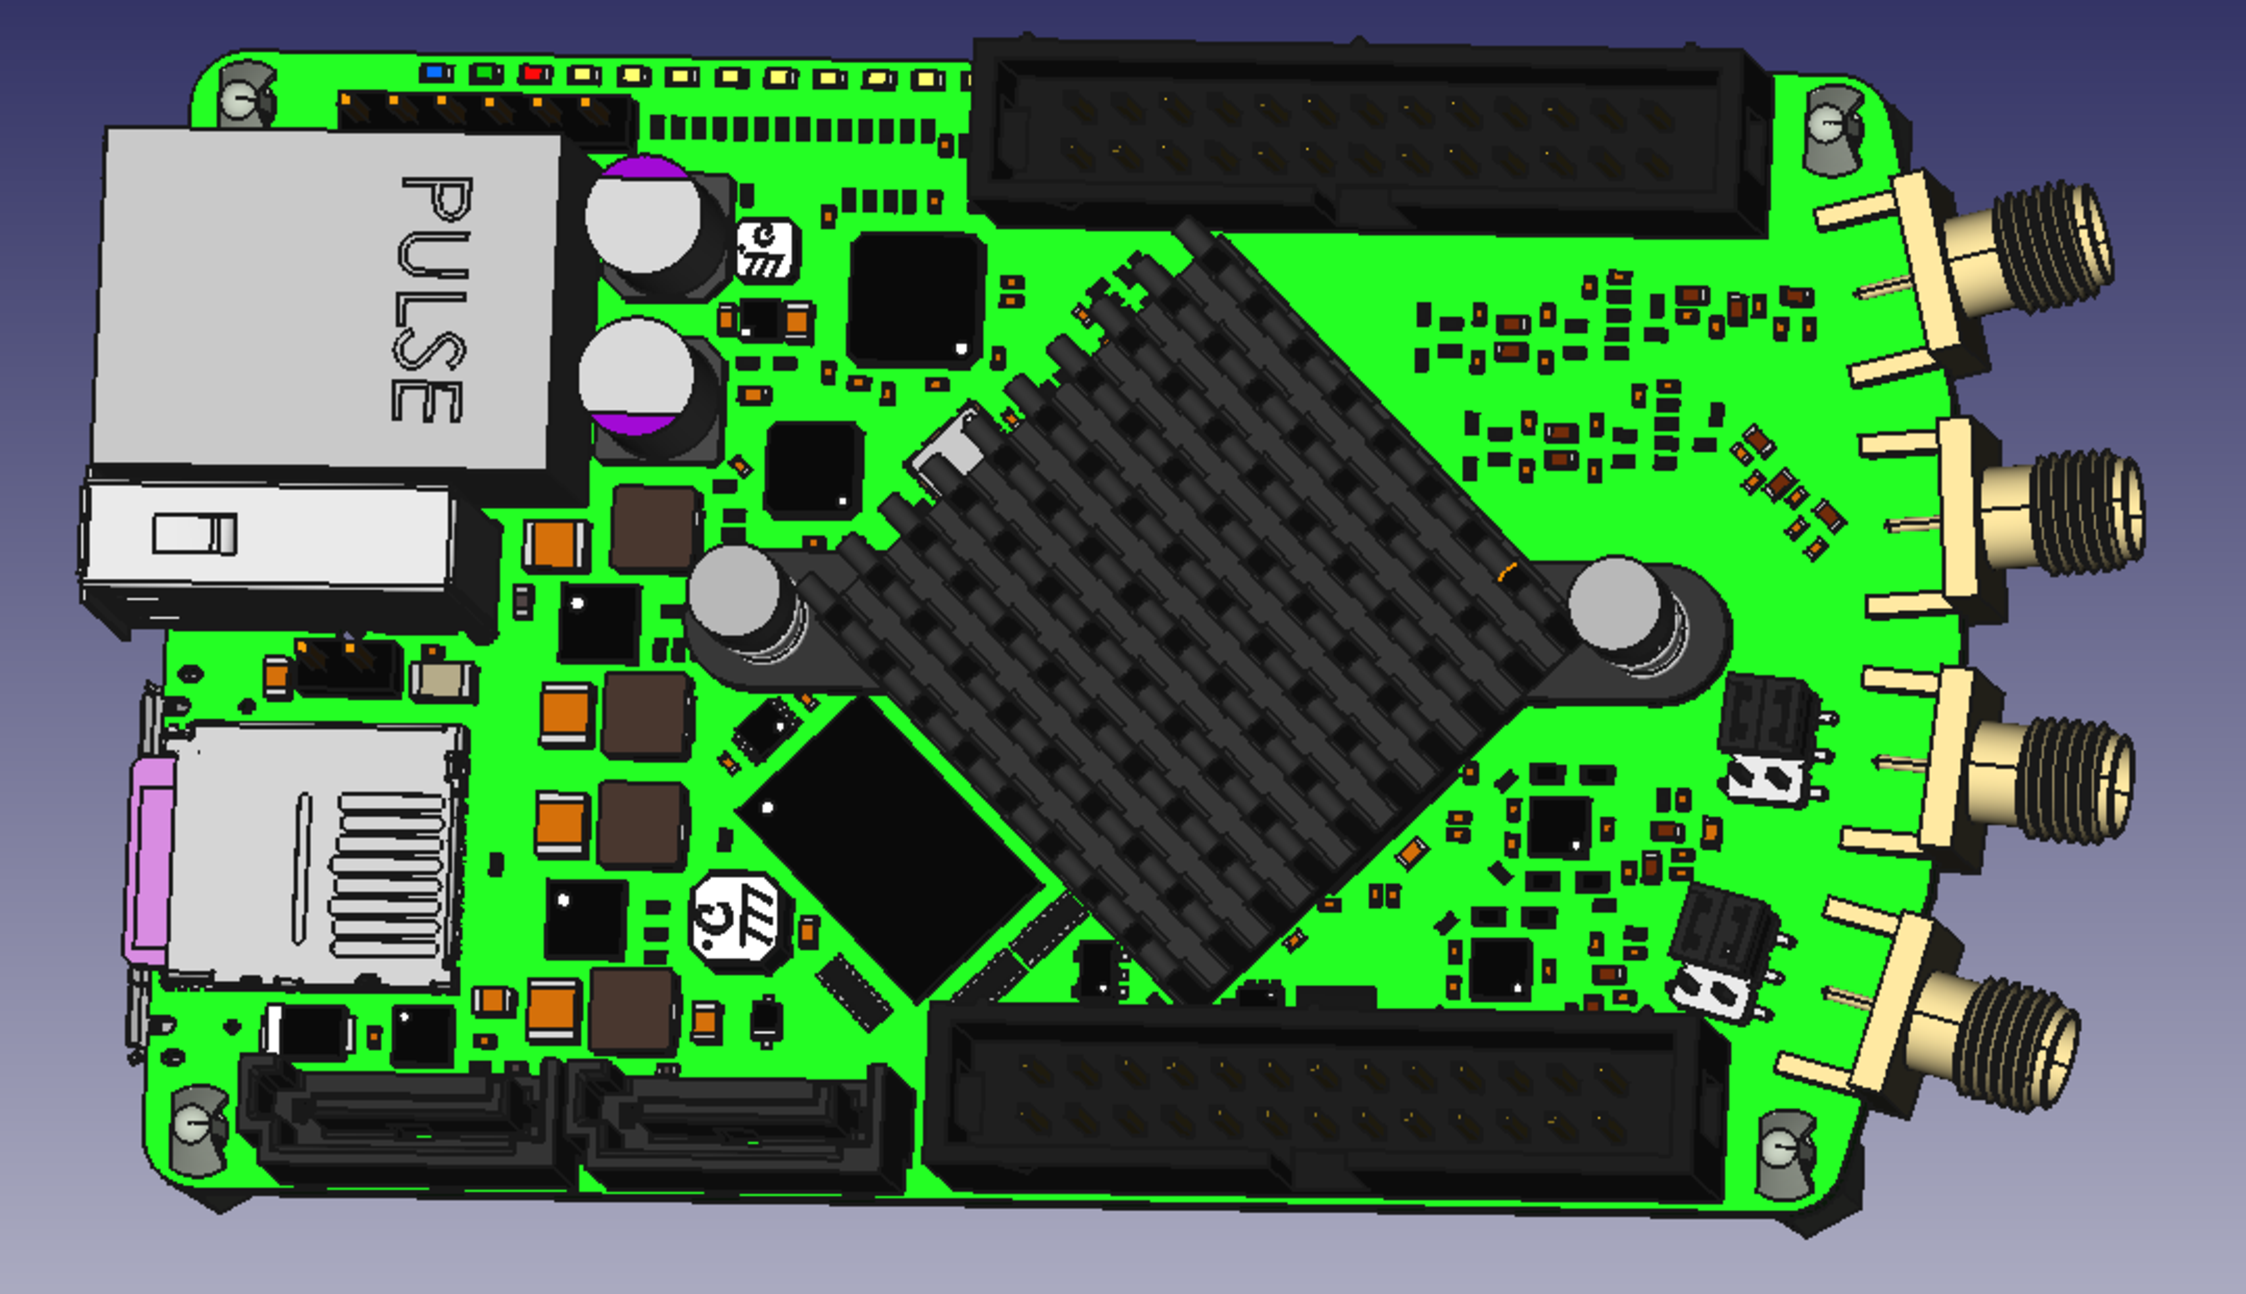
\includegraphics[angle=90,width=0.75\textwidth]{rp_freecad_up}}
	 \end{column}
	\end{columns}
\end{frame} 

%\begin{frame}
%	\frametitle{Futuro: RedPitaya}
%		\begin{block}{}
%	  	\begin{itemize}
%	    	\item Esperamos tener el sistema listo para fin de año (2016) o mediados
%							del año que viene
%	    	\item Es poca la ganancia en ancho de banda, respecto a lo que ya
%							tenemos. Pero se gana mucho en flexibilidad.
%	    	\item Todavía hay que trabajar, tanto en hardware como en software
%				\item ... pero para eso estamos dentro de una comunidad... y el \alert{trabajo
%							colaborativo} debe afianzarse
%	  	\end{itemize}
%		\end{block}
%\end{frame} 

\begin{frame}
	\frametitle{Hardware}
		\begin{exampleblock}{Características}
			\begin{itemize}
							\item Procesador $\to$ \alert{Xilinx Zynq-7010 SoC ARM dual core
											CPU y FPGA Artix 7}
				\item RAM $\to$ 512\,MB
				\item Rango dinámico de conversión de +1\,V a -1\,V
				\item Acceso $\to$ USB console, Ethernet, WiFi dongle
				\item Potencia $\to$ 5V x 2A max., 0.9A typ.
				\item Fast ADC $\to$ \alert{Dual channel, 14-bit, 125\,MSPS}
				\item Fast ADC $\to$ \alert{Dual channel, 14-bit, 125\,MSPS}
				\item Otros I/Os $\to$ DAC lento x 4, ADC lento ($\sim$125\,kHz) x 4,
								digital I/O digitales x 16, conector daisy chain 
			\end{itemize}
		\end{exampleblock}
\end{frame}

\begin{frame}
				\frametitle{Diferencias}
  \begin{block}{}
    \centering
    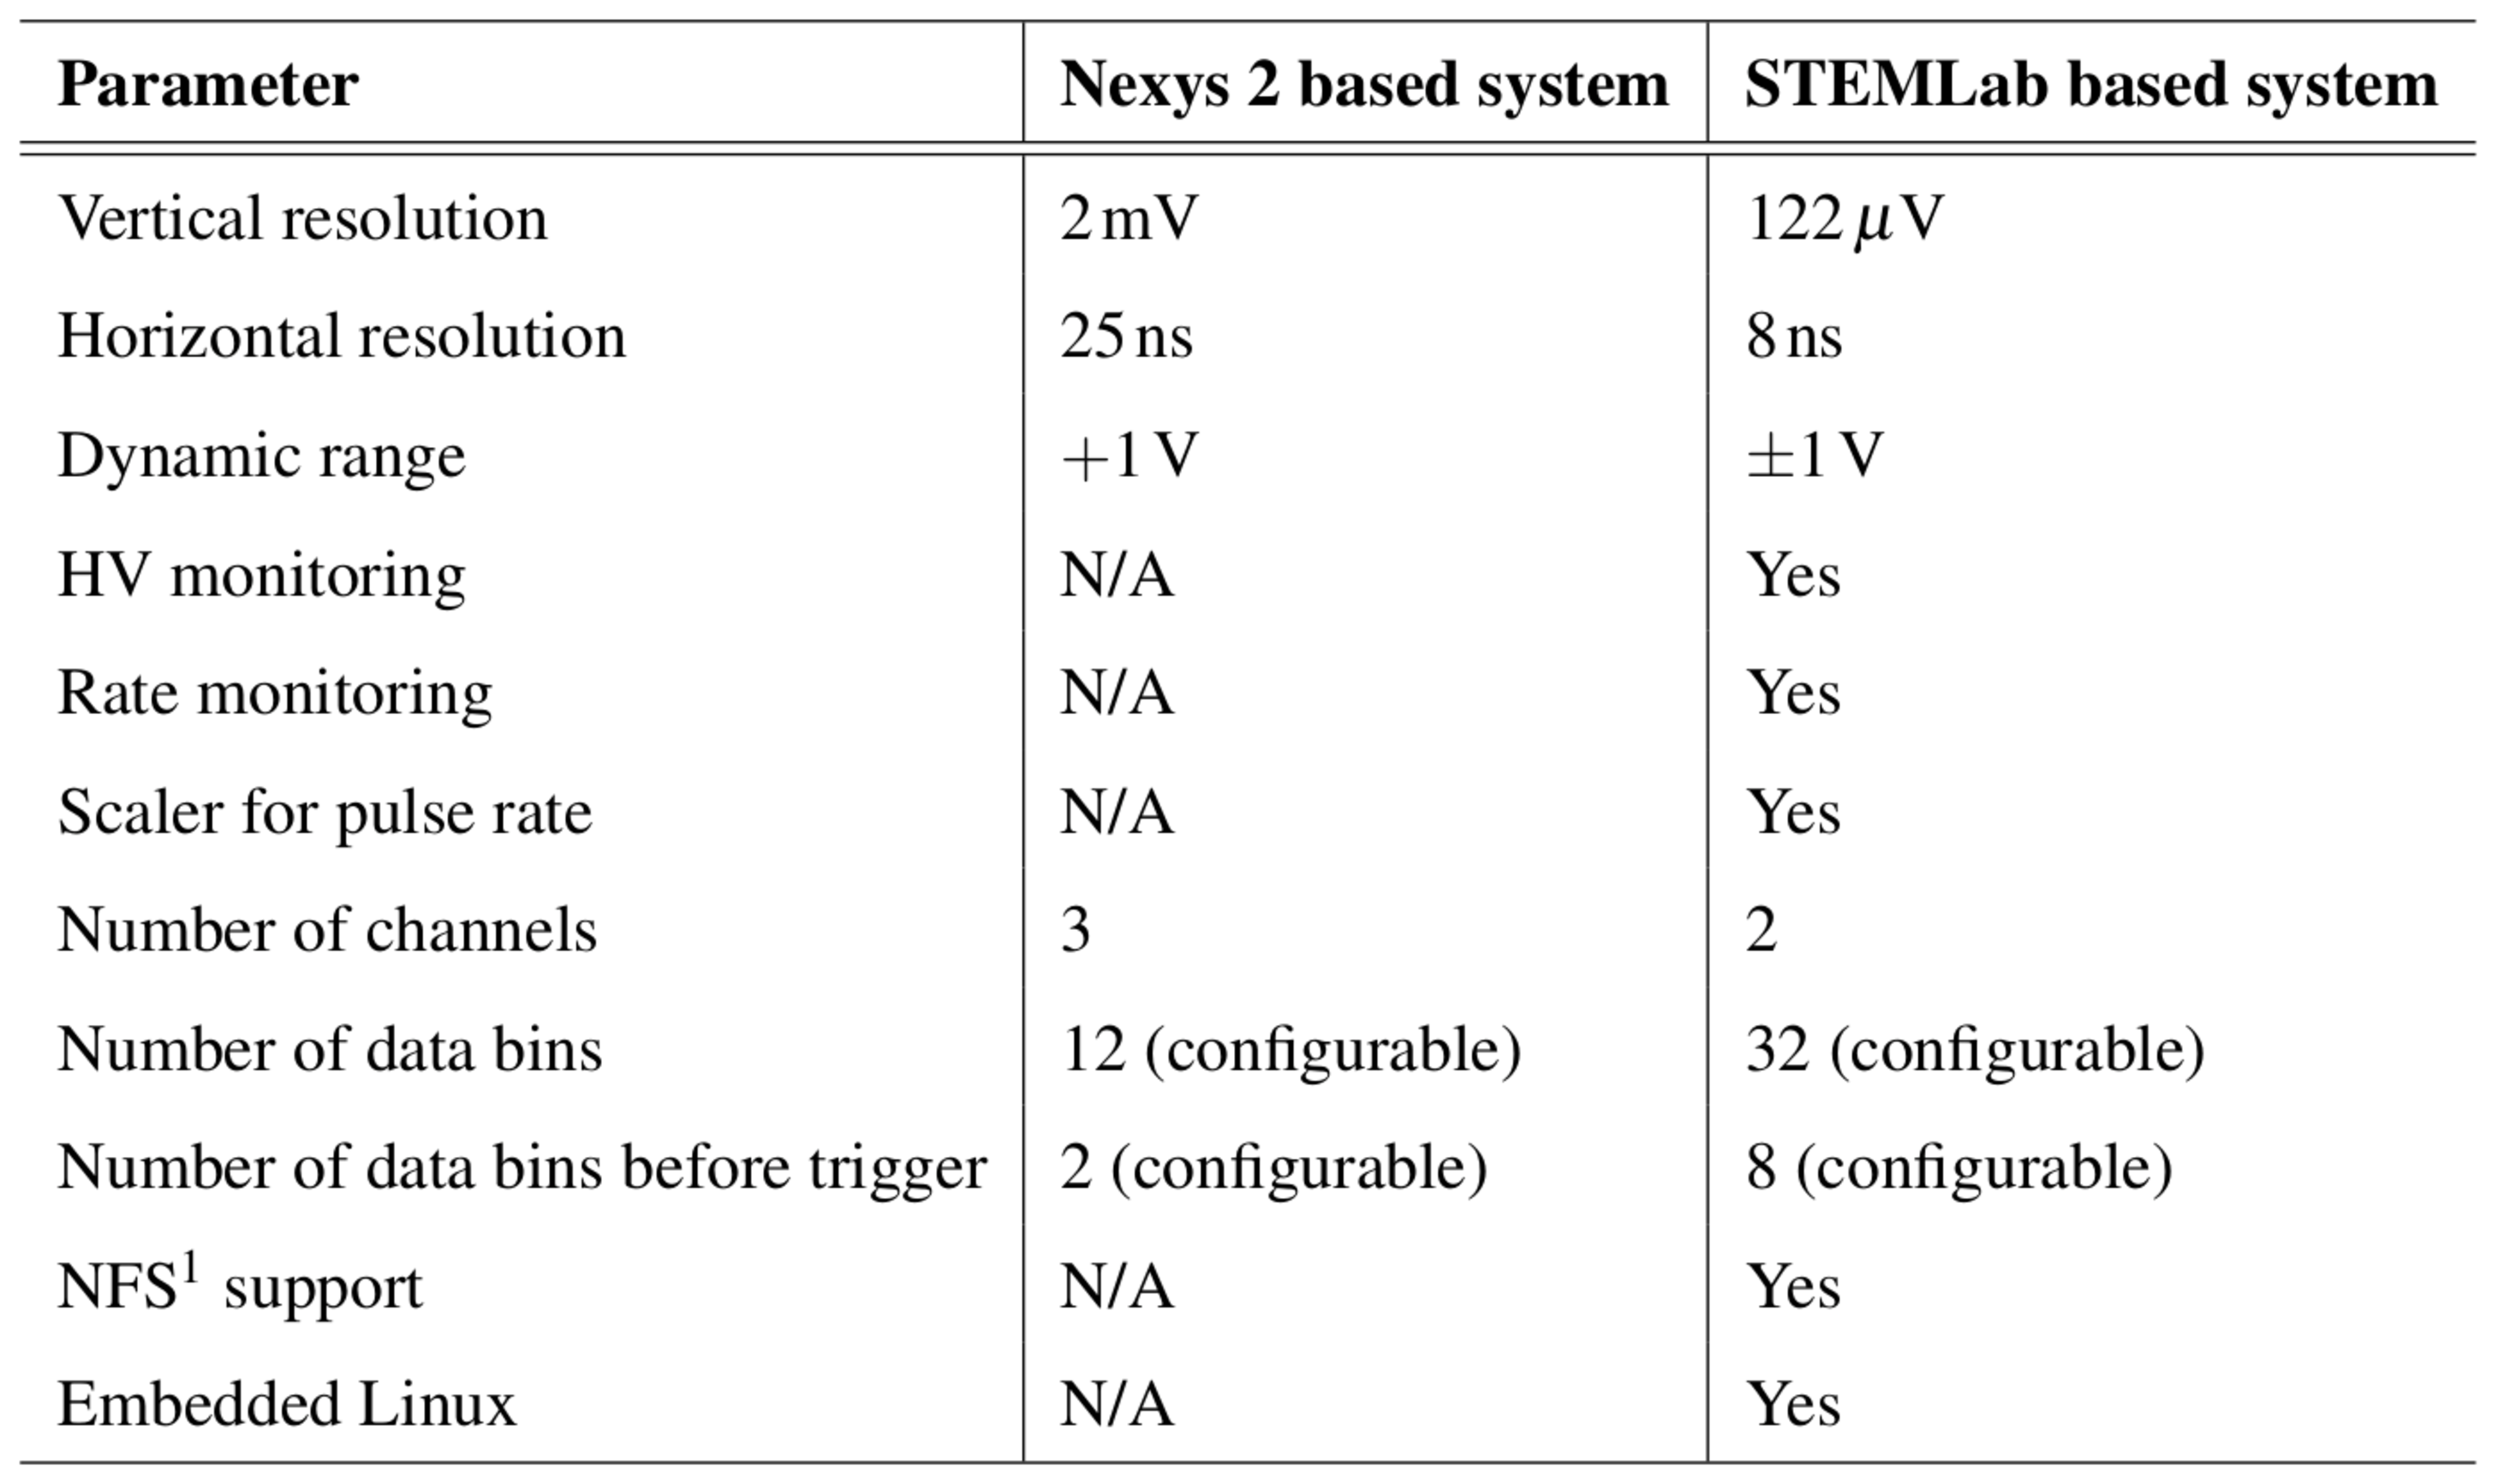
\includegraphics[width=0.9\textwidth]{diferencias_nexys_rp}
  \end{block}
\end{frame}

\begin{frame}
				\frametitle{El firmware}
  \begin{block}{}
    \centering
    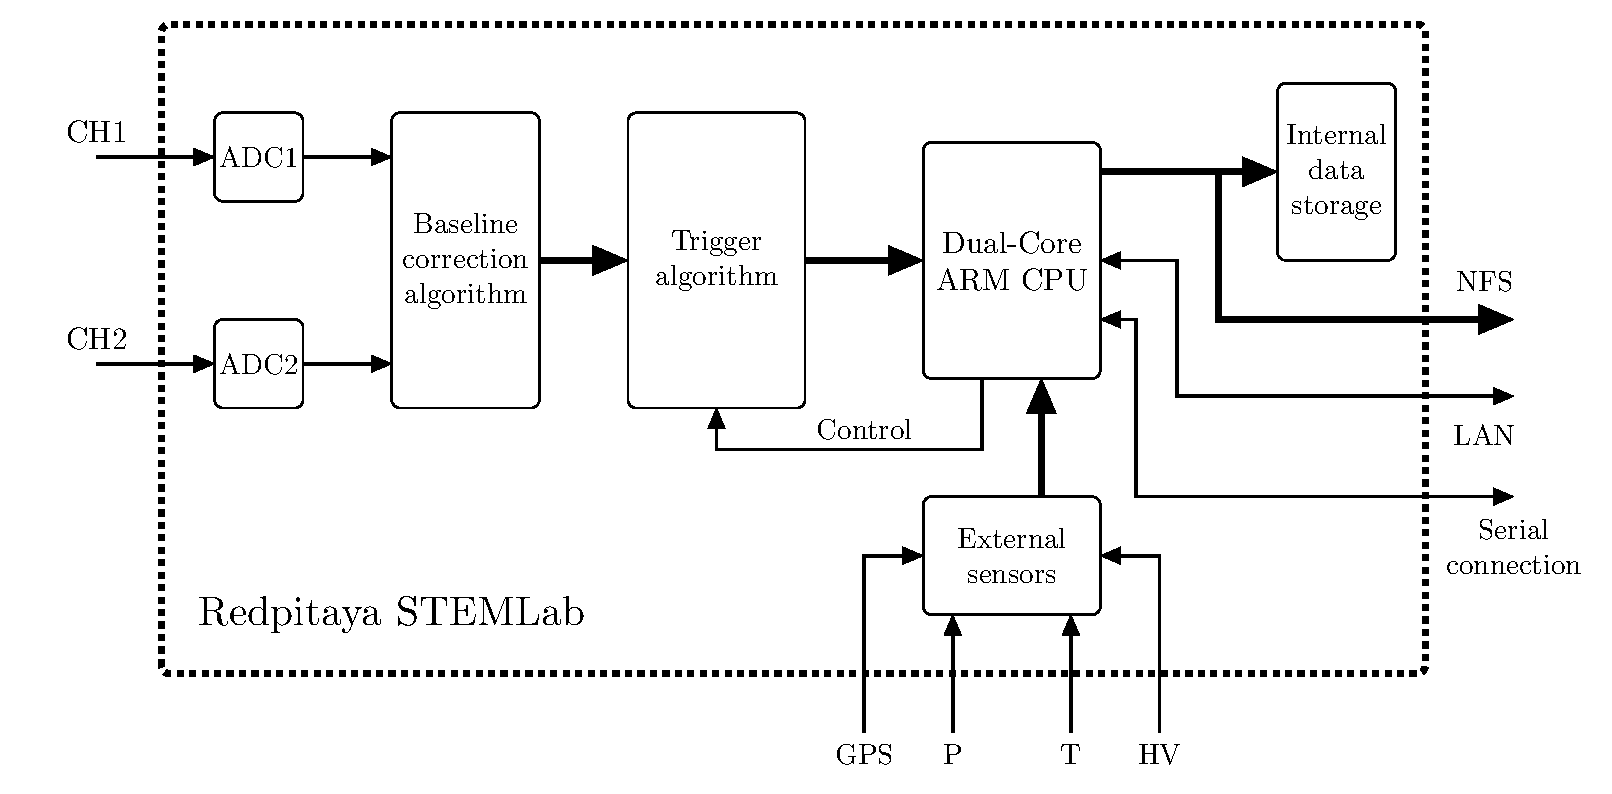
\includegraphics[width=0.9\textwidth]{diag_sys}
  \end{block}
\end{frame}

\begin{frame}
				\frametitle{Corrección (digital) de la línea de base}
  \begin{block}{}
    \centering
					\boxed{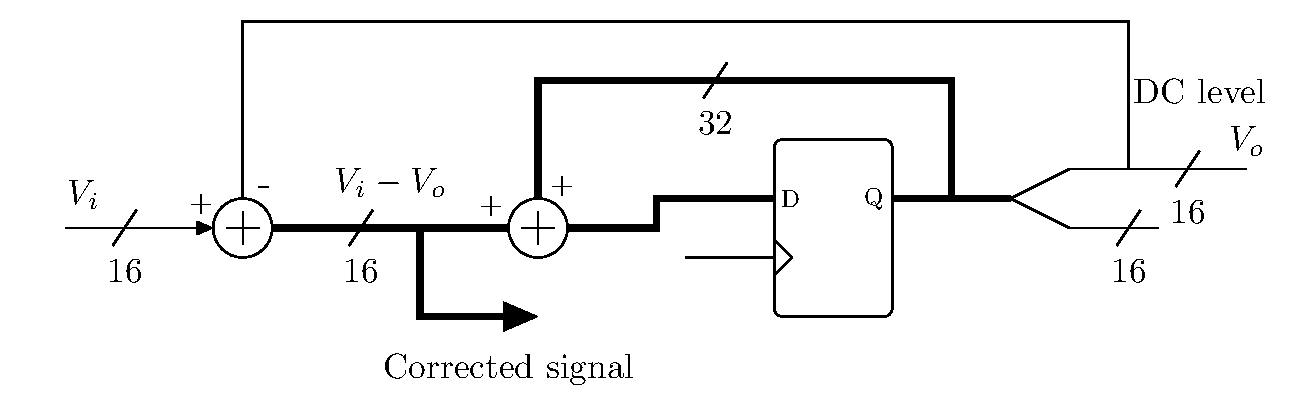
\includegraphics[width=0.9\textwidth]{dc_removal}} \\
    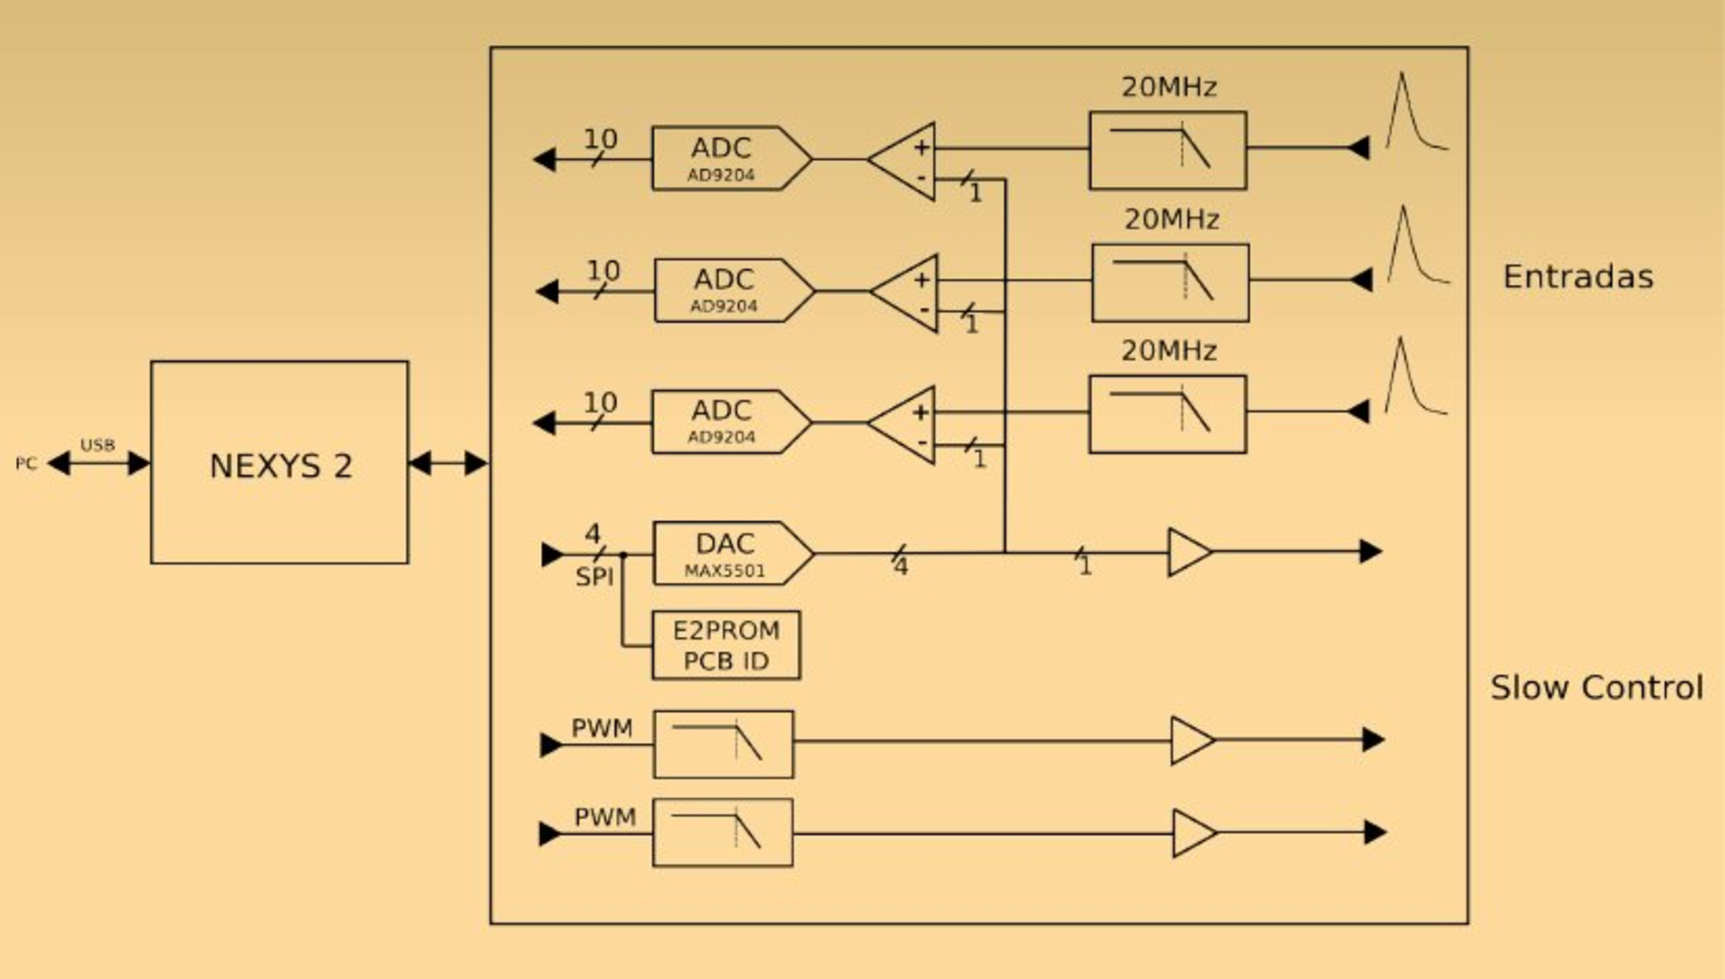
\includegraphics[width=0.7\textwidth]{diagrama_en_bloques_lago}
  \end{block}
\end{frame}

\begin{frame}
				\frametitle{Corrección (digital) de la línea de base}
  \begin{block}{}
    \centering
					\boxed{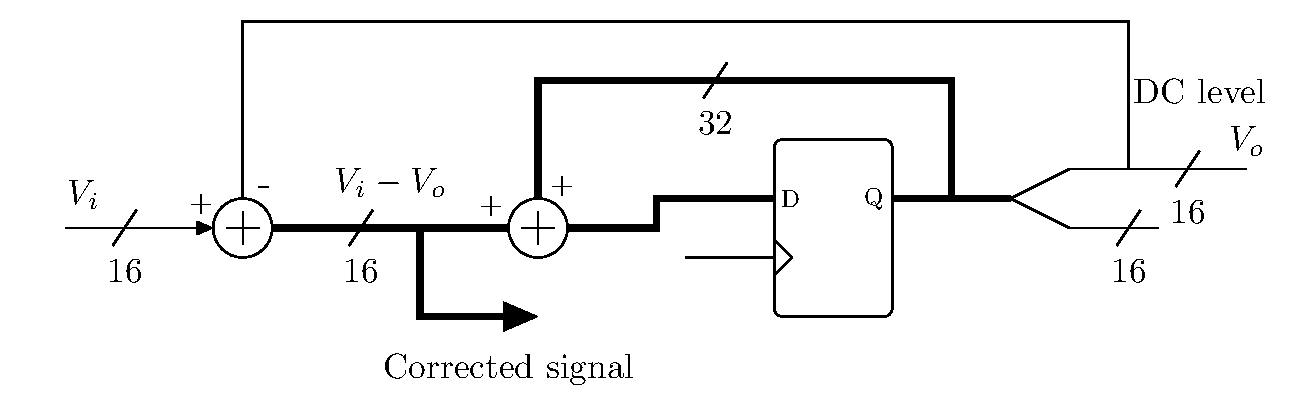
\includegraphics[width=0.9\textwidth]{dc_removal}} \\
					\boxed{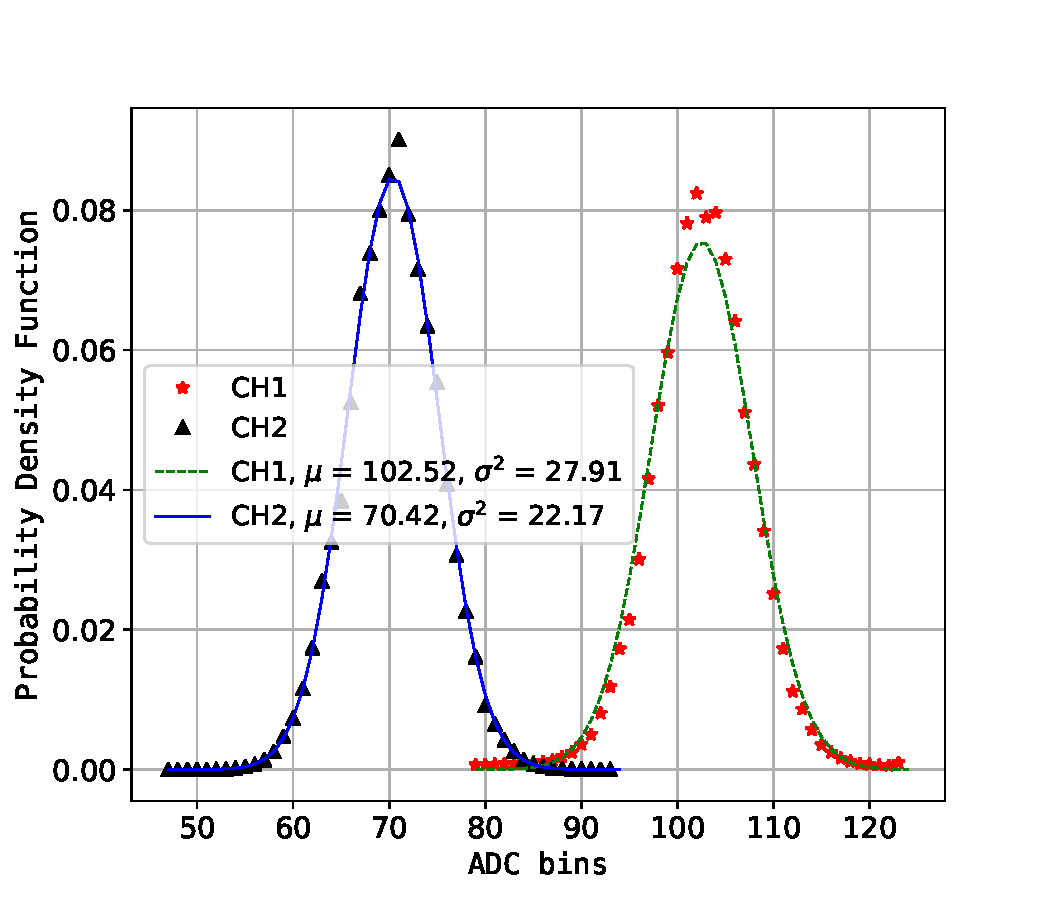
\includegraphics[width=0.4\textwidth]{baselines_sin_corregir}} 
					\boxed{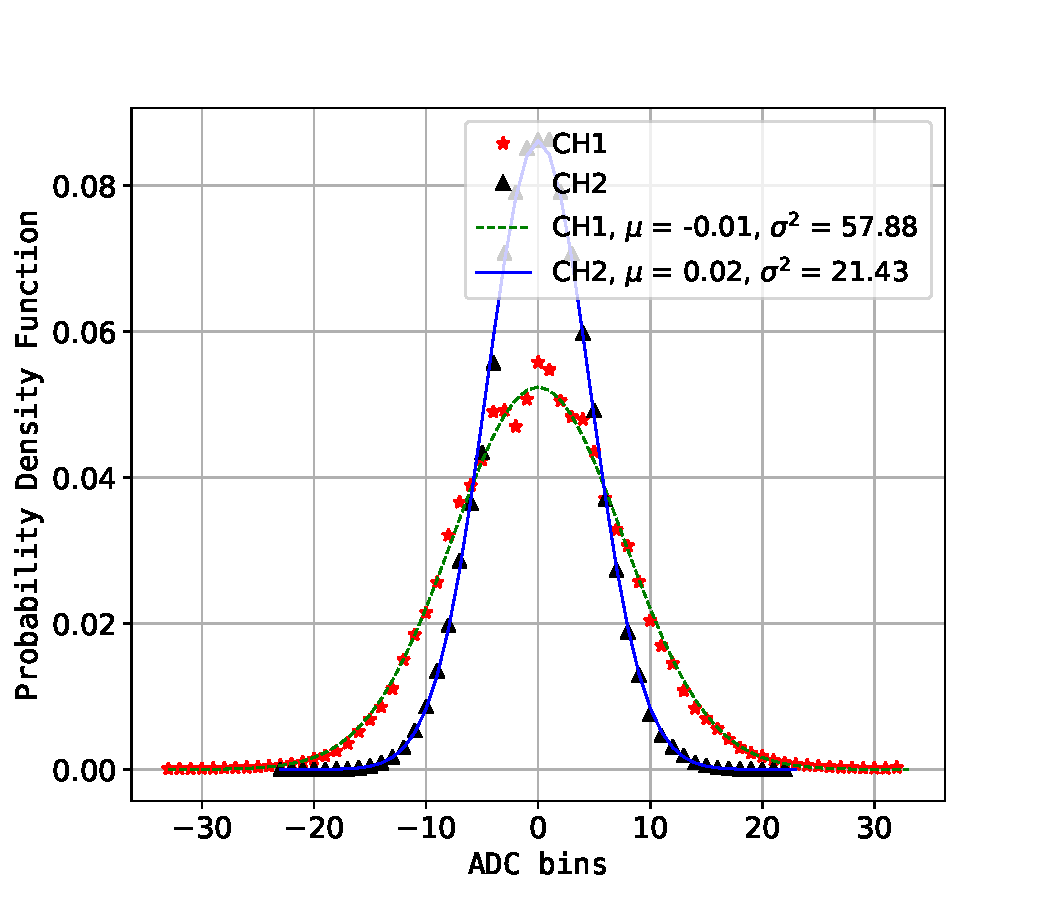
\includegraphics[width=0.4\textwidth]{baselines_corregidas}} 
  \end{block}
\end{frame}

\begin{frame}
				\frametitle{Placa hija \alert{RP\_CTRL\_BOARD v1r0}}
	\begin{columns}
		\begin{column}{0.50\textwidth}
	  	\fbox{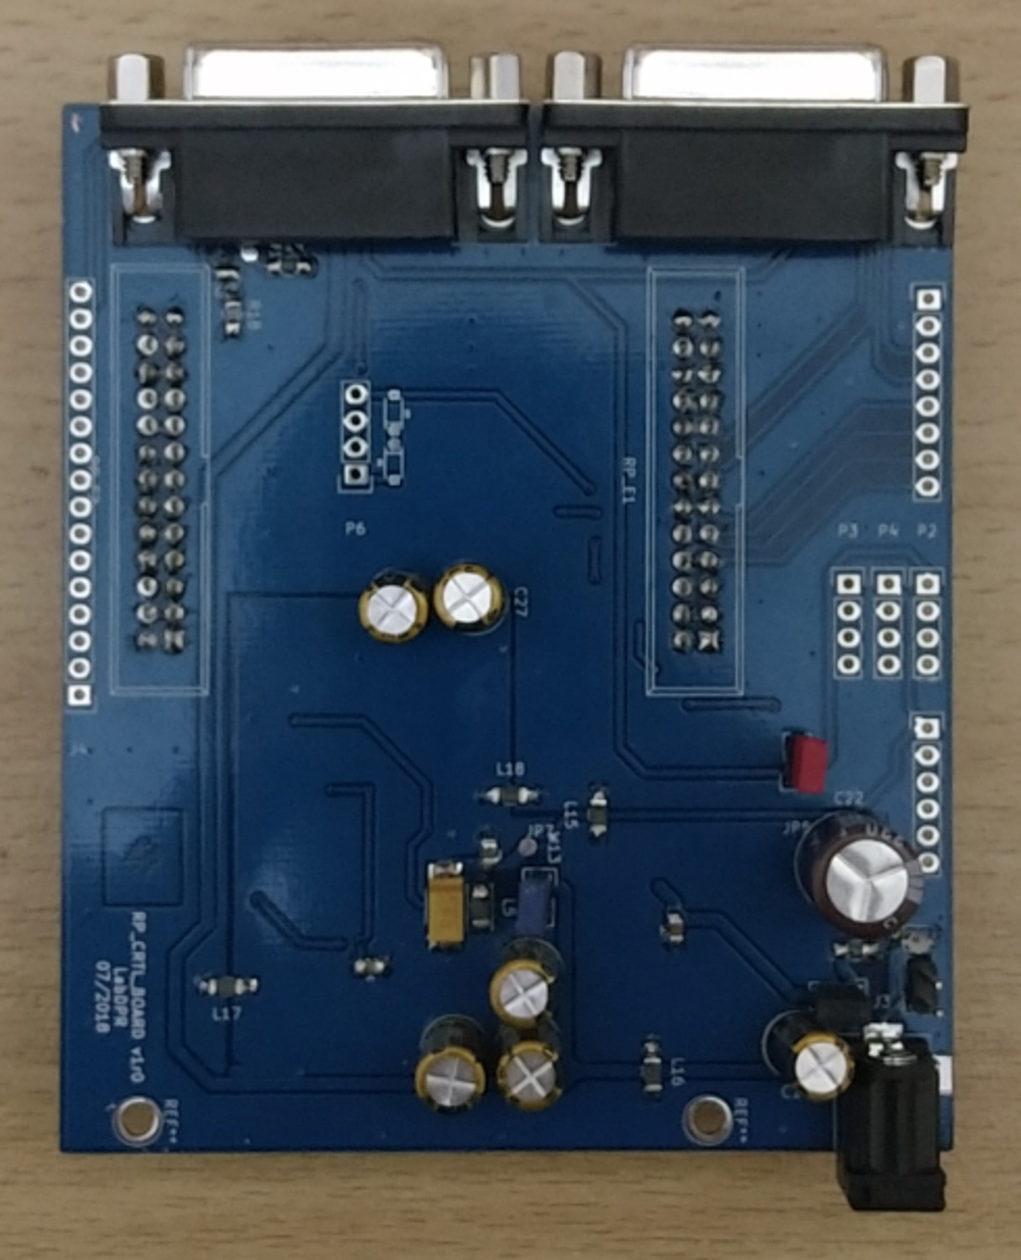
\includegraphics[width=0.9\textwidth]{placa_arriba}}
		\end{column} 
	 	\begin{column}{0.5\textwidth}
	  	\fbox{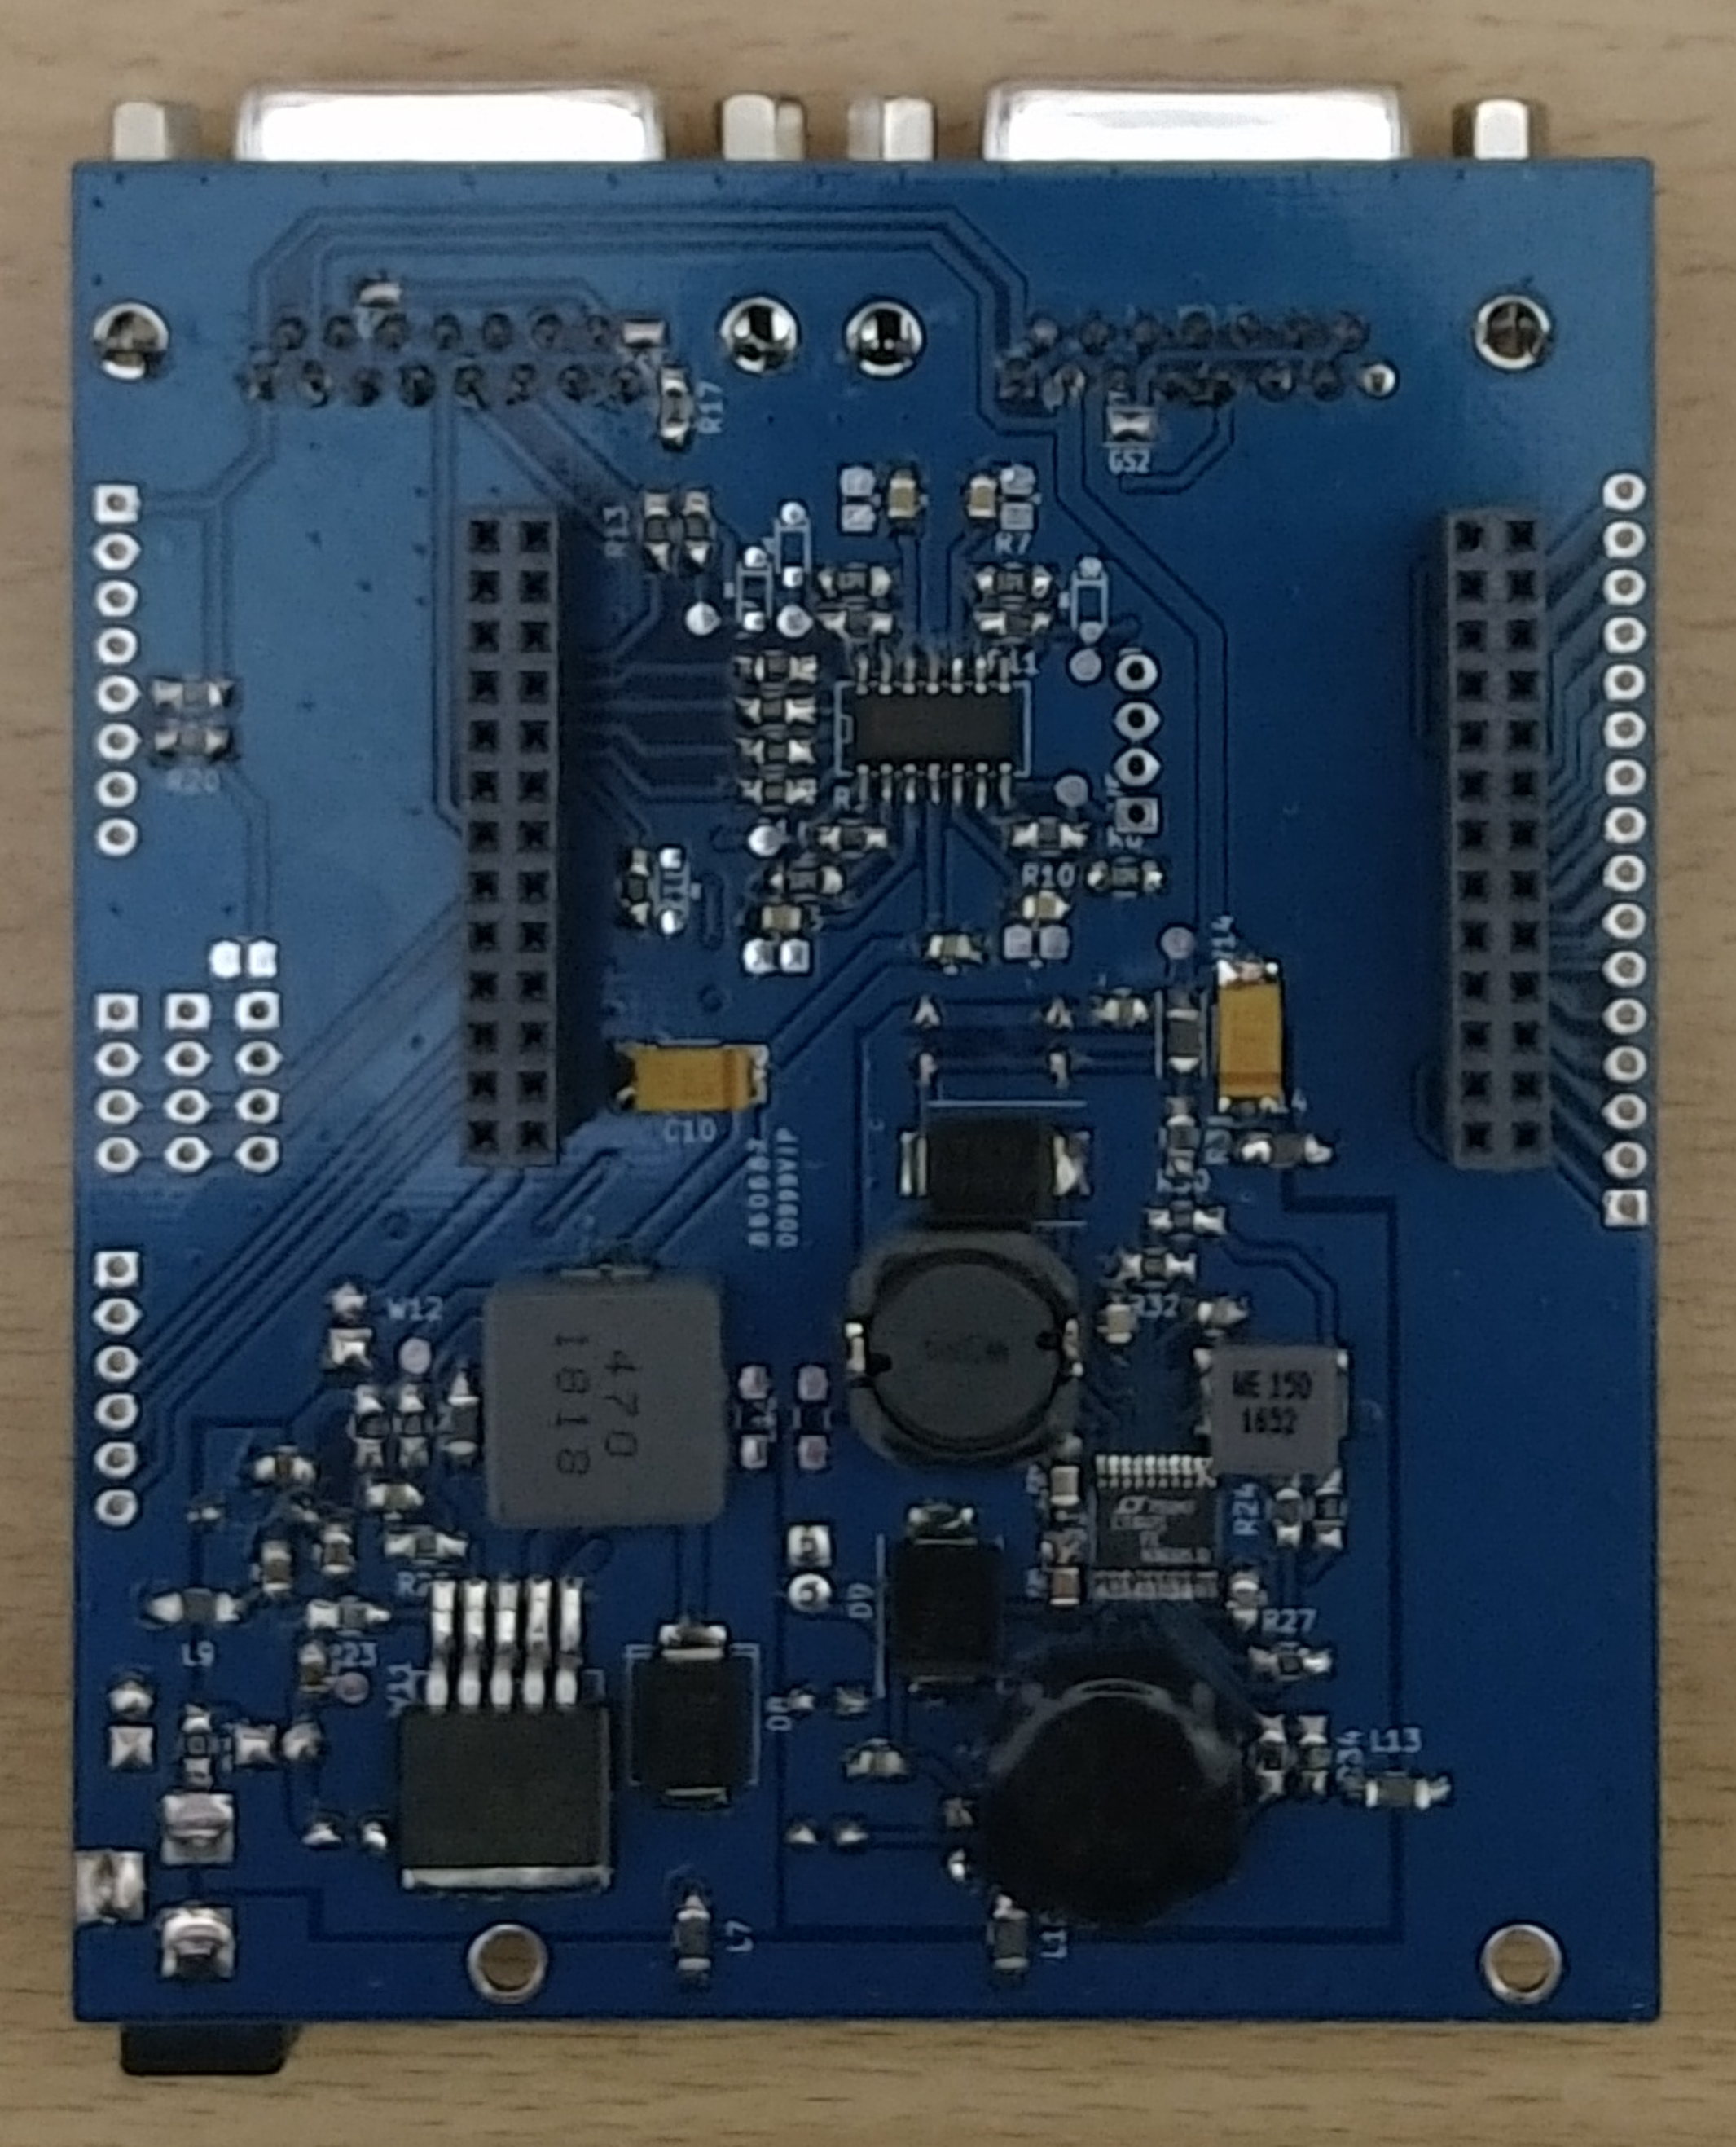
\includegraphics[width=0.9\textwidth]{placa_abajo}}
	 \end{column}
	\end{columns}
\end{frame}

\begin{frame}
	\frametitle{Hardware}
				\begin{exampleblock}{Características}
			\begin{itemize}
				\item Conectores DB15 $\to$ conexión directa a las bases de los PMT
				\item Permite la configuración de las HV en las bases de los PMT
				\item Monitoreo de HV
				\item Monitoreo de temperatura interna y externa
				\item Provee todas las tensiones (y potencia) necesaria para alimentar:
								\begin{itemize}
												\item La RedPitaya $\to$ \alert{+5\,V}
												\item La base del PMT $\to$ \alert{+12\,V, $\pm$3.3\,V,
																+5\,V}
												\item Los sensores (PyT, GPS, etc.) $\to$
																\alert{+3.3\,V, +5\,V}
								\end{itemize}
				\item Funciona con una única fuente de +12\,V @ 2\,A
				\item Permite sensar/colocar hasta 2 tensiones extras
				\item Permite interconectar sensores con diferentes protocolos (IIC,
								UART, SPI) a la RP
			\end{itemize}
		\end{exampleblock}
\end{frame}

\begin{frame}
				\frametitle{Primeros resultados}
	\begin{columns}
		\begin{column}{0.50\textwidth}
	  	\fbox{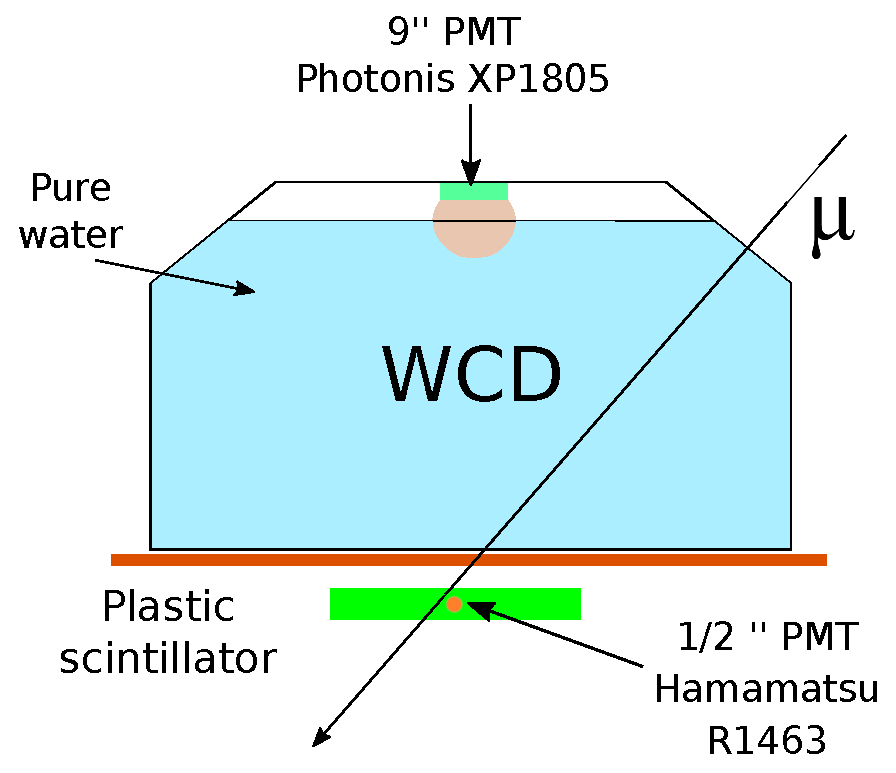
\includegraphics[width=0.95\textwidth]{detectorscheme}}
		\end{column} 
	 	\begin{column}{0.5\textwidth}
						\fbox{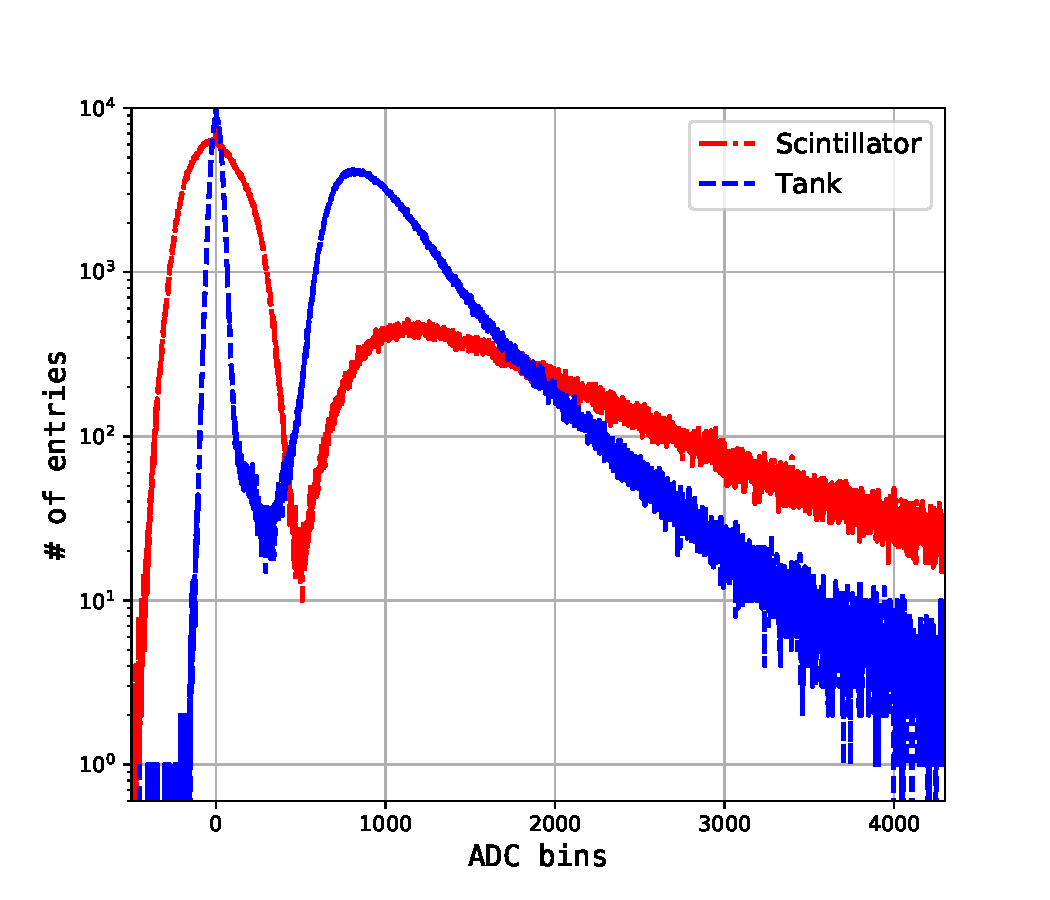
\includegraphics[width=0.95\textwidth]{boy_cente_chrg_tot}}
	 \end{column}
	\end{columns}
\end{frame}

\begin{frame}
				\frametitle{Primeros resultados}
	\begin{columns}
		\begin{column}{0.50\textwidth}
	  	\fbox{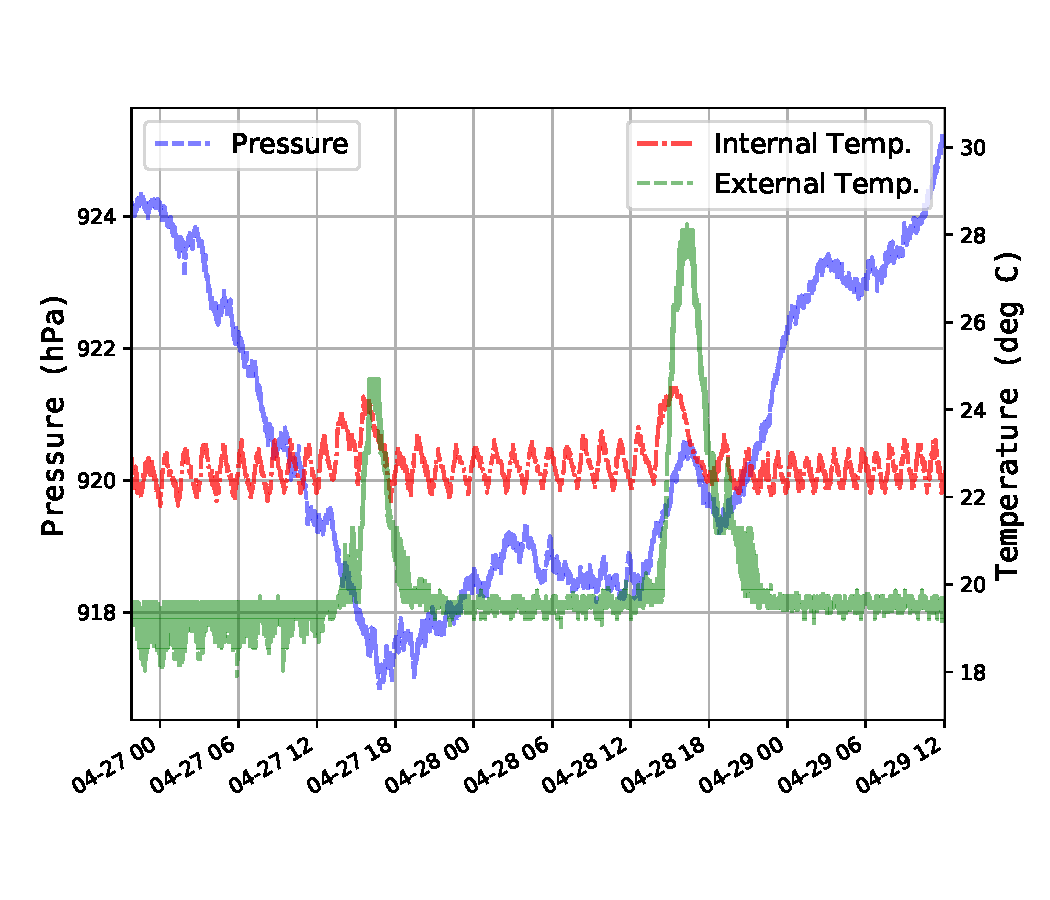
\includegraphics[width=0.95\textwidth]{temp_pres_sensing}}
		\end{column} 
	 	\begin{column}{0.5\textwidth}
						\fbox{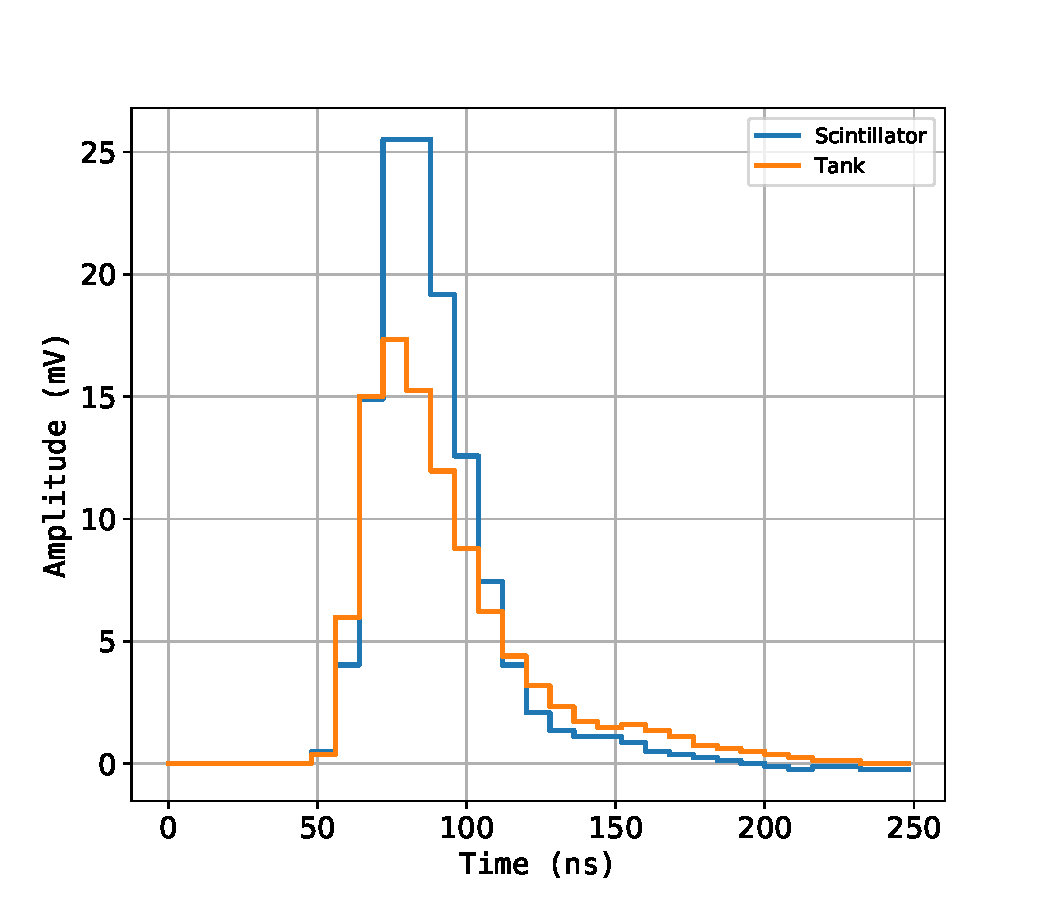
\includegraphics[width=0.95\textwidth]{boy_cente_pprom_total}}
	 \end{column}
	\end{columns}
\end{frame}

\begin{frame}
	\frametitle{Trabajo futuro}
		\begin{exampleblock}{}
			\begin{itemize}
				\item Integración GPS $\to$ GPSBee o similar 
				\item Medición estable por largo tiempo (meses, años)
				\item Sistema de sincronismo automático con servidores de datos y entre
								placas (Linux, flexible)
				\item Agregar funcionamiento por interrupciones (parcialmente
								implementado)
				\item Software de adquisición?
				\item Trabajar en la documentación y con los repositorios de datos
				\item Posibles algoritmos de procesamiento adicionales que surjan de la
								Comunidad
				\item Integración ANNA, etc.
				\item \alert{Que la comunidad LAGO empiece a usarlo!}
			\end{itemize}
		\end{exampleblock}
\end{frame}

%%------------------------------------------------------------------------------
%\section{Las electrónicas}
%%------------------------------------------------------------------------------
%\begin{frame}
%  \begin{center}
%    \Huge{\color{blue}{Las electrónicas: \\ El firmware de la FPGA}}
%  \end{center}
%\end{frame}
%
%\subsection{El firmware FPGA}
%
%\begin{frame}
%  \frametitle{¿Qué cosa es el firmware?}
%    \begin{block}{}
%      \begin{itemize}
%        \pause
%        \item Es el conjunto de instrucciones que realizan el ordenamiento de la
%              lógica interna de la FPGA de acuerdo a las necesidades del caso.
%        \pause
%        \item Está compuesto por bloques de código escrito en VHDL/Verilog
%          \begin{itemize}
%            \item VHDL $\rightarrow$ VHSIC Hardware Description Language
%            \item Verilog $\rightarrow$ Sintaxis similar a C/C++
%          \end{itemize}
%        \pause
%        \item Es el encargado de sincronizar todas las tareas que va a realizar
%              la FPGA y dicta cómo lo va a llevar adelante.
%        \pause
%        \item Se ocupa de la comunicación con el mundo exterior a la FPGA.
%      \end{itemize}
%    \end{block}
%\end{frame}
%
%\begin{frame}
%  \frametitle{¿Con qué herramientas contamos?}
%  \begin{block}{}
%    \begin{itemize}
%      \item  FPGA, Nexys2
%        \begin{itemize}
%          \item Este es nuestro caso, pero podría usarse otra
%                FPGA/marca, de acuerdo a las necesidades.
%        \end{itemize}
%      \item  ISE-Webpack, VIVADO (Xilinx)
%      \begin{itemize}
%        \item
%http://www.xilinx.com/products/design-tools/ise-design-suite/ise-webpack.html
%        \item www.xilinx.com/products/design-tools/vivado.html
%      \end{itemize}
%      \item  Make
%      \item  LibFPGALink, Git
%      \begin{itemize}
%        \item Librerías para el manejo del puerto USB (Chip EZ-USB FX2LP de
%							Cypress)
%        \item https://github.com/makestuff/libfpgalink
%      \end{itemize}
%      \item  Mercurial, Bitbucket
%      \begin{itemize}
%        \item Control de versiones
%        \item https://bitbucket.org/lago/lago-fpga-vhdl
%      \end{itemize}
%    \end{itemize}
%\end{block}
%\end{frame}
%
%\begin{frame}
%\frametitle{Las herramientas}
%  \begin{columns}
%    \begin{column}{0.45\textwidth}
%      \begin{block}{Nexys2}
%        \begin{itemize}
%          \item  Familia FPGA Spartan3E
%          \item  60 pines E/S disponibles para nuestro uso (144 en total)
%          \item  El firmware LAGO ocupa aprox. el 70\% de sus recursos internos
%                 (memoria, bloques de I/O, etc.)
%        \end{itemize}
%      \end{block}
%    \end{column} 
%    \begin{column}{0.65\textwidth}
%      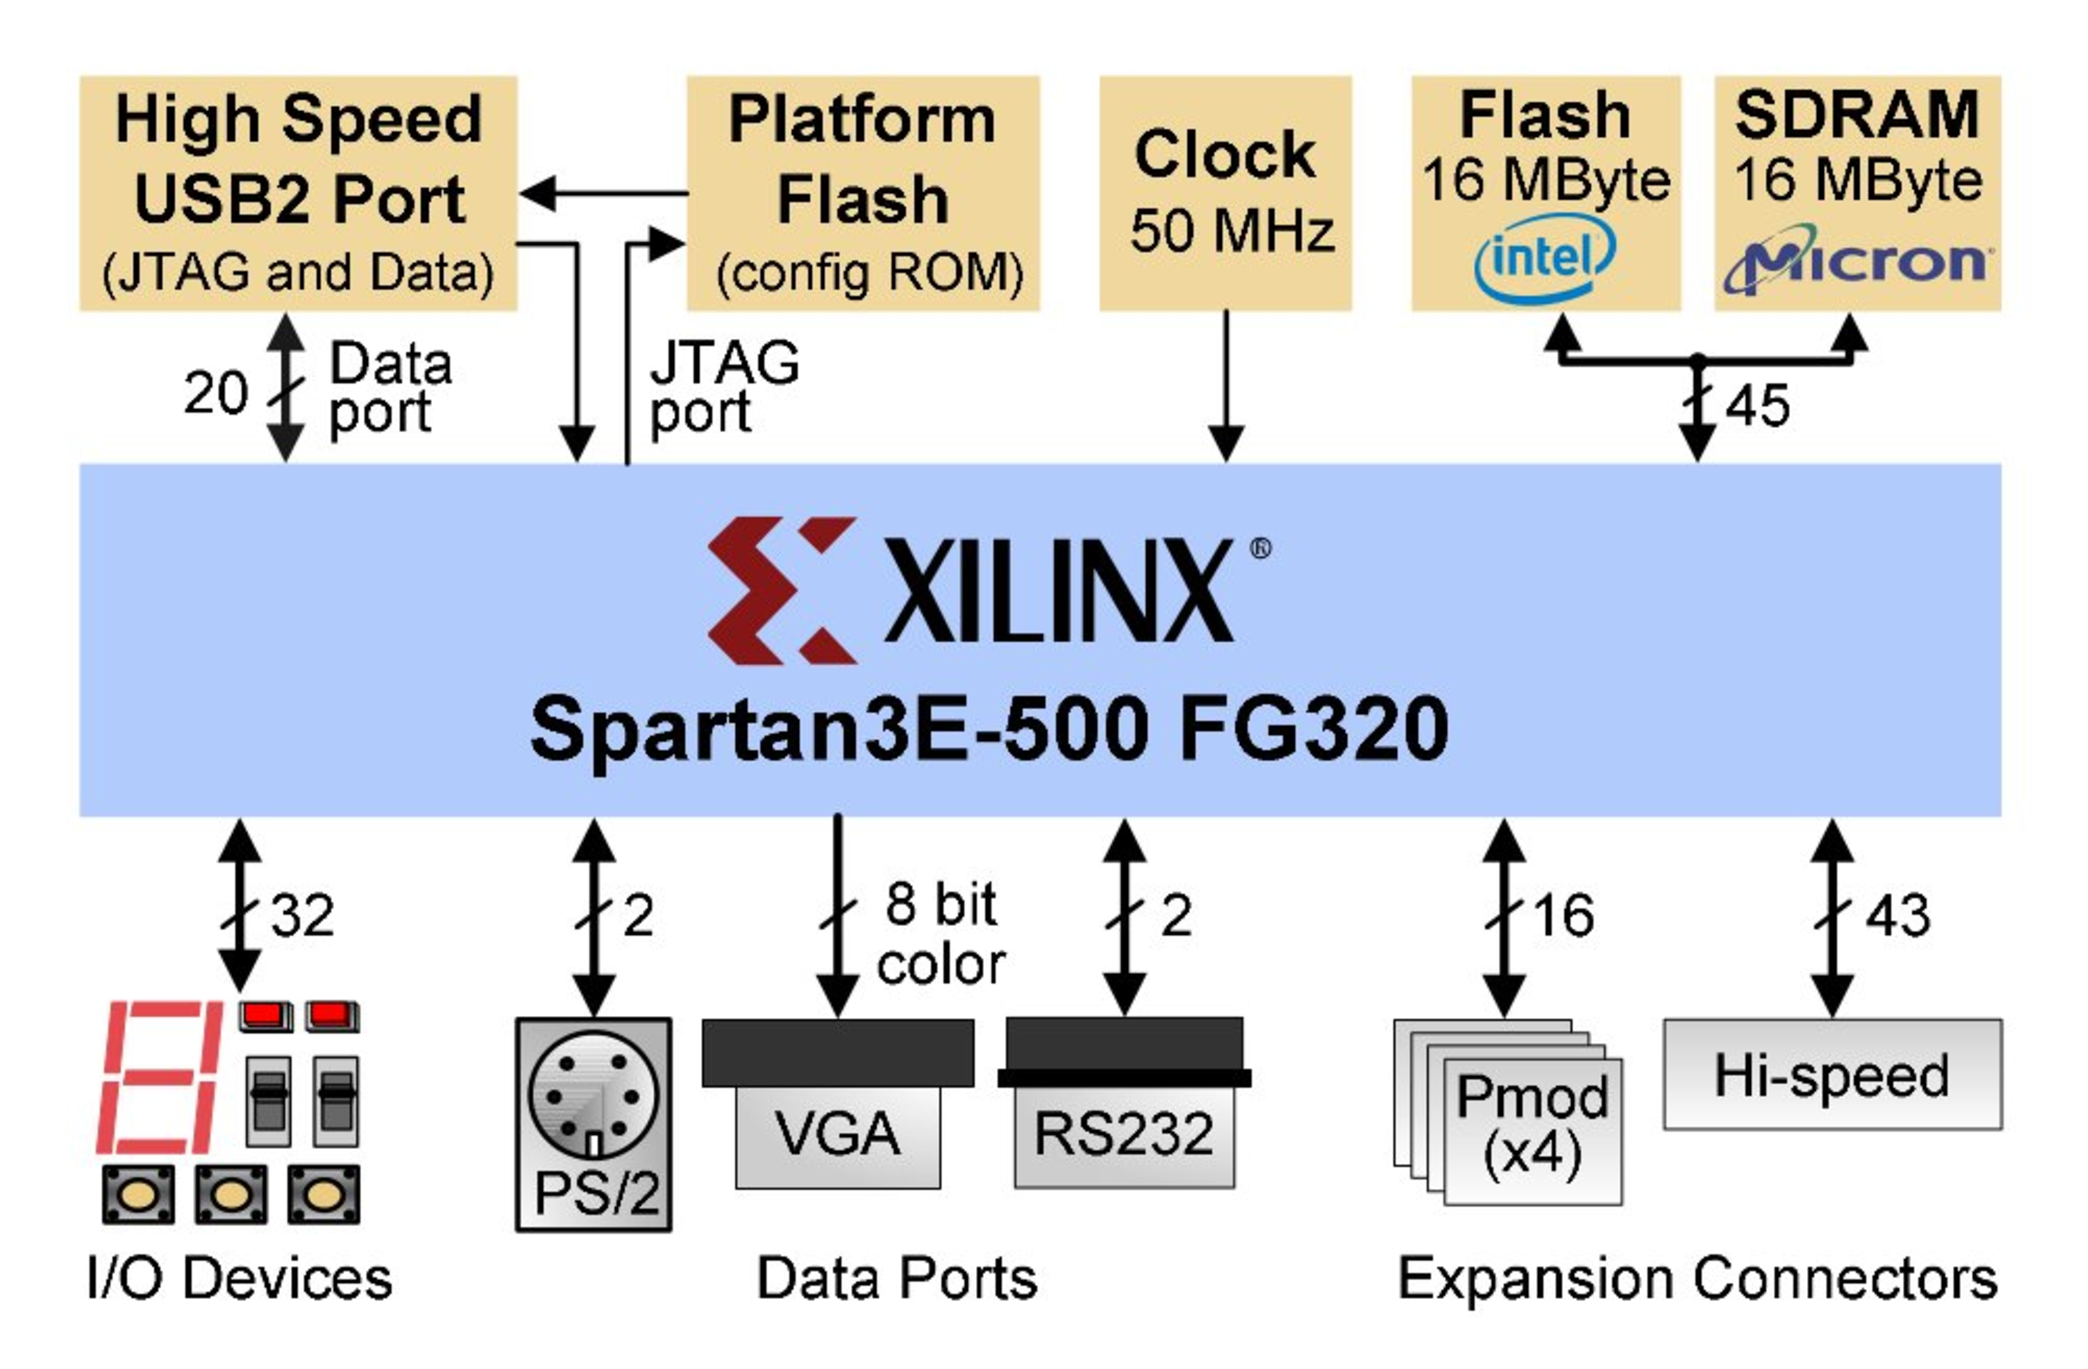
\includegraphics[width=0.8\textwidth]{bloques_nexys2}
%    \end{column}
%  \end{columns}
%\end{frame}
%
%\subsubsection{Una visión general sobre el sistema}
%
%\begin{frame}
%  \frametitle{Los bloques dentro de la FPGA}
%  \begin{block}{}
%    \centering
%    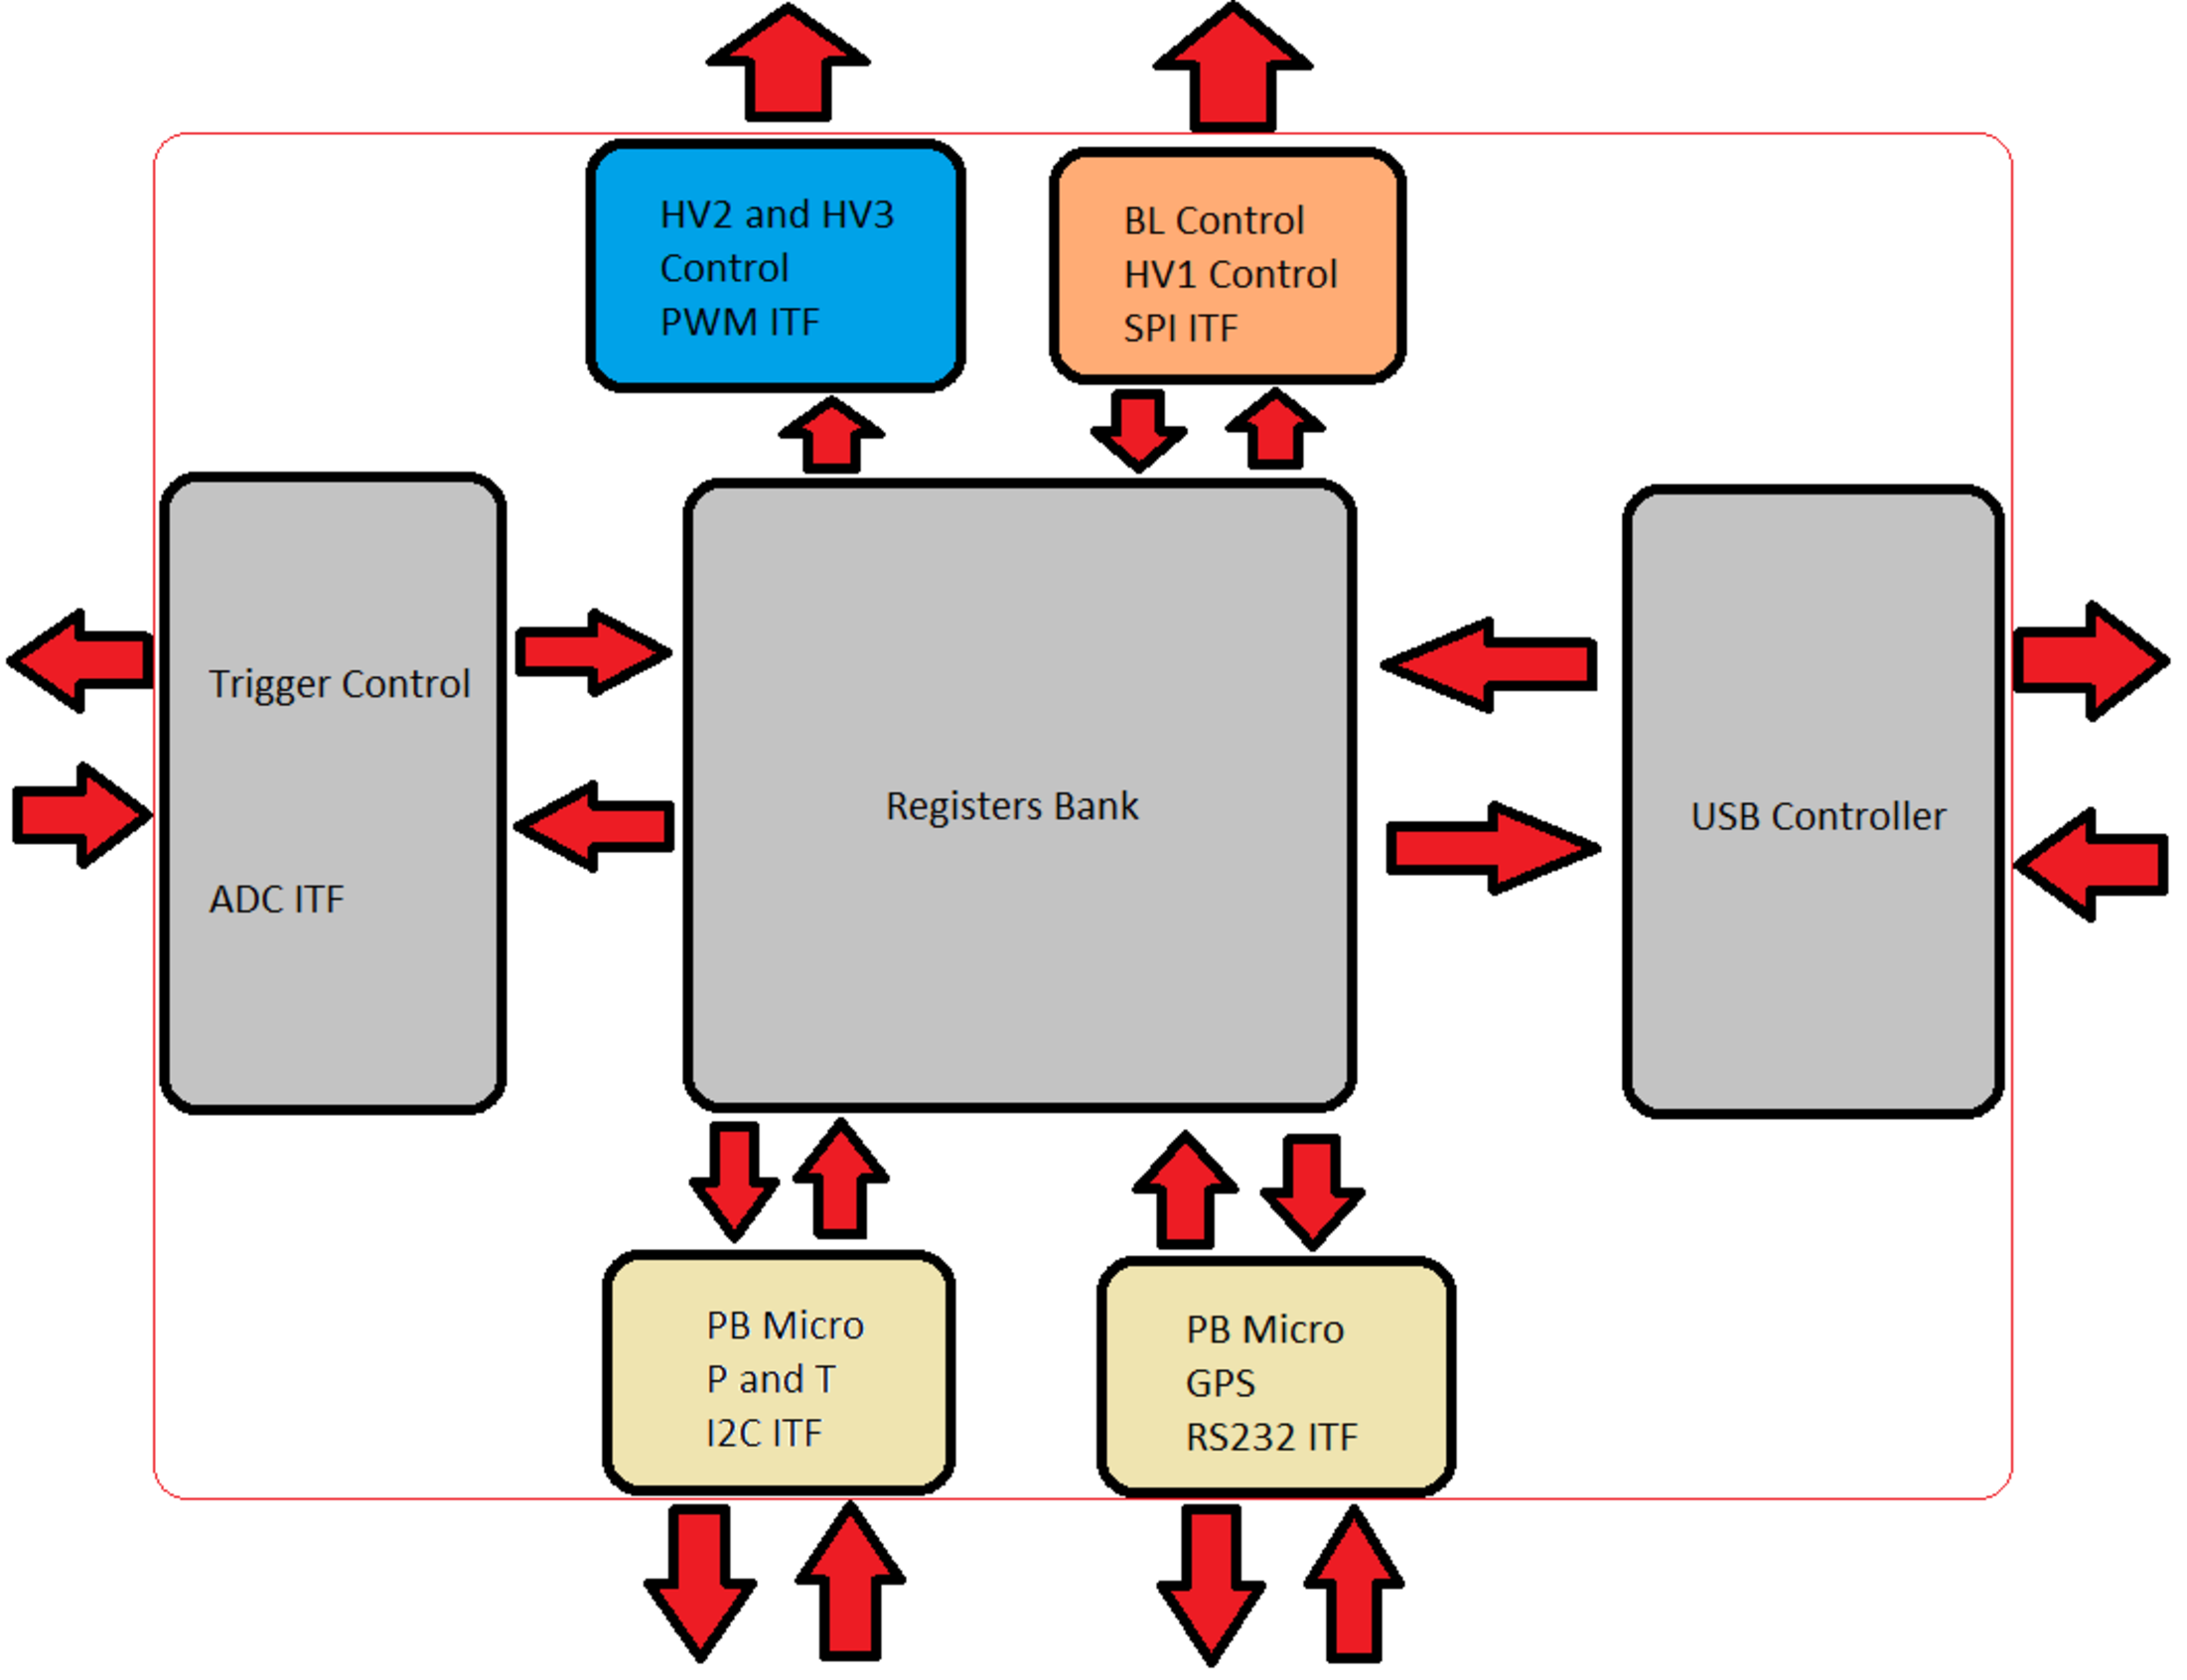
\includegraphics[height=0.75\textheight,width=0.75\textwidth]{bloques_fpga_lago}
%  \end{block}
%\end{frame}
%
%%\begin{frame}
%%  \frametitle{La jerarquía dentro del firmware}
%%  \begin{block}{}
%%    \centering
%%    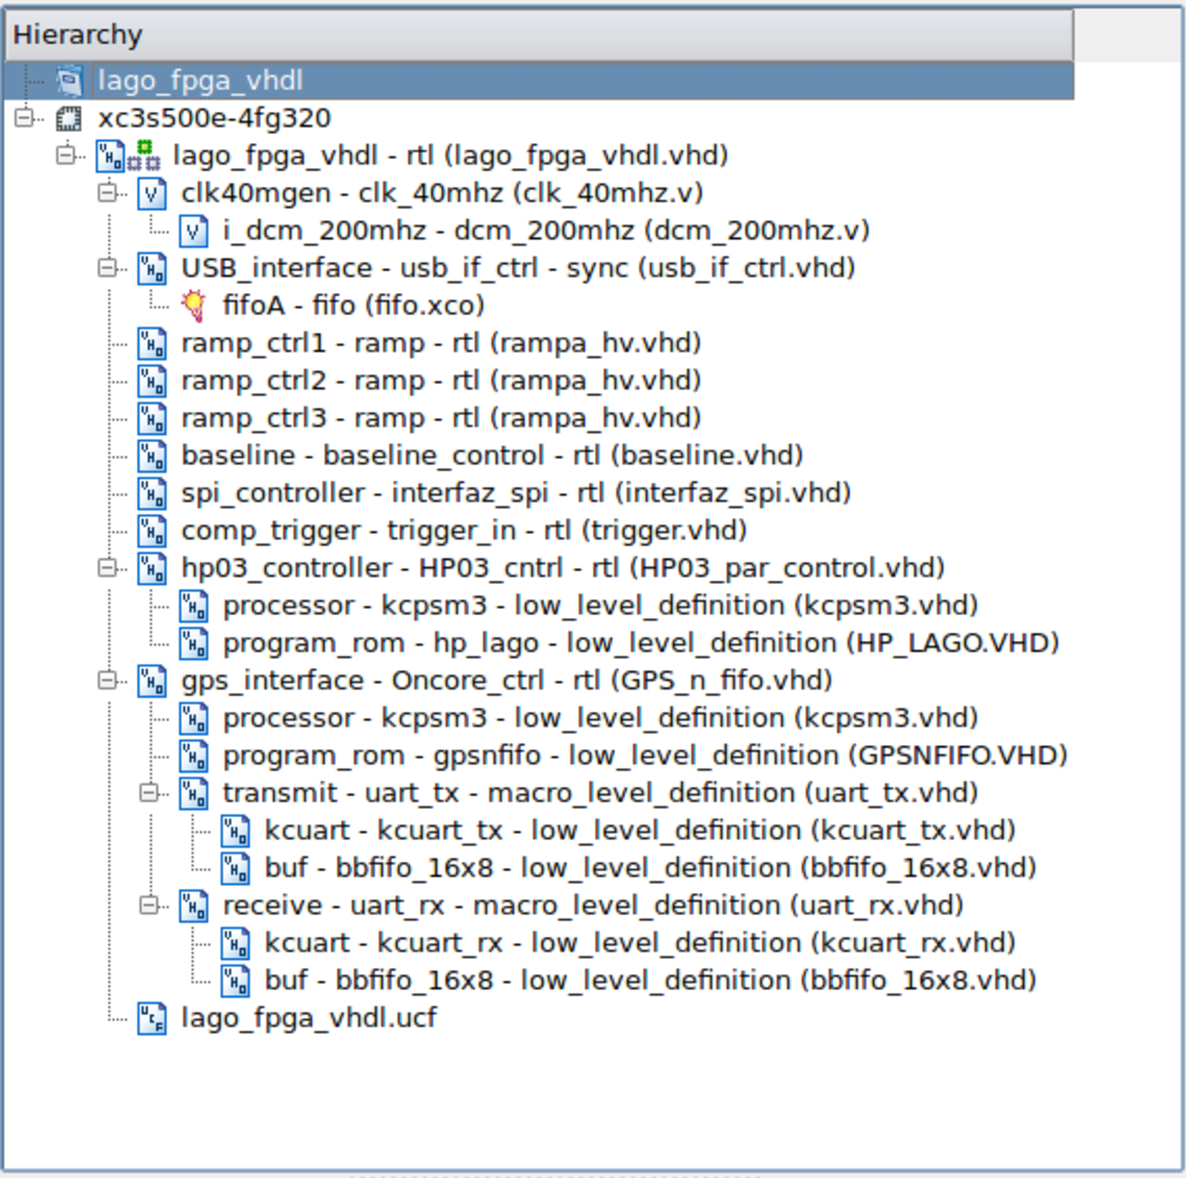
\includegraphics[height=0.75\textheight,width=0.75\textwidth]{jerarquia_lago}
%%  \end{block}
%%\end{frame}
%
%\subsubsection{Una visión general sobre el firmware}
%
%%\begin{frame}
%%  \frametitle{Un punto importante dentro del firmware}
%%    \begin{block}{El $\mu$C PicoBlaze}
%%      \begin{itemize}[<+->]
%%        \item  $\mu$C propiedad de Xilinx (exclusivo para FPGA de esta marca)
%%        \item  Programación en Assembler
%%        \item  KCPSM $\rightarrow$ (K)constant Coded Programmable State
%%               Machine
%%        \item  Flexibilidad para manejo de puertos estándares (RS-232, $I^2C$,
%%               etc.)
%%        \item  Necesidad de implementar controladores genéricos en
%%               VHDL/Verilog para independizarnos de las marcas (y del
%%							 Assembler!!).
%%      \end{itemize}
%%    \end{block}
%%\end{frame}
%%
%%\begin{frame}
%%  \frametitle{Un punto importante dentro del firmware}
%%  \begin{block}{El $\mu$C PicoBlaze}
%%    \centering
%%    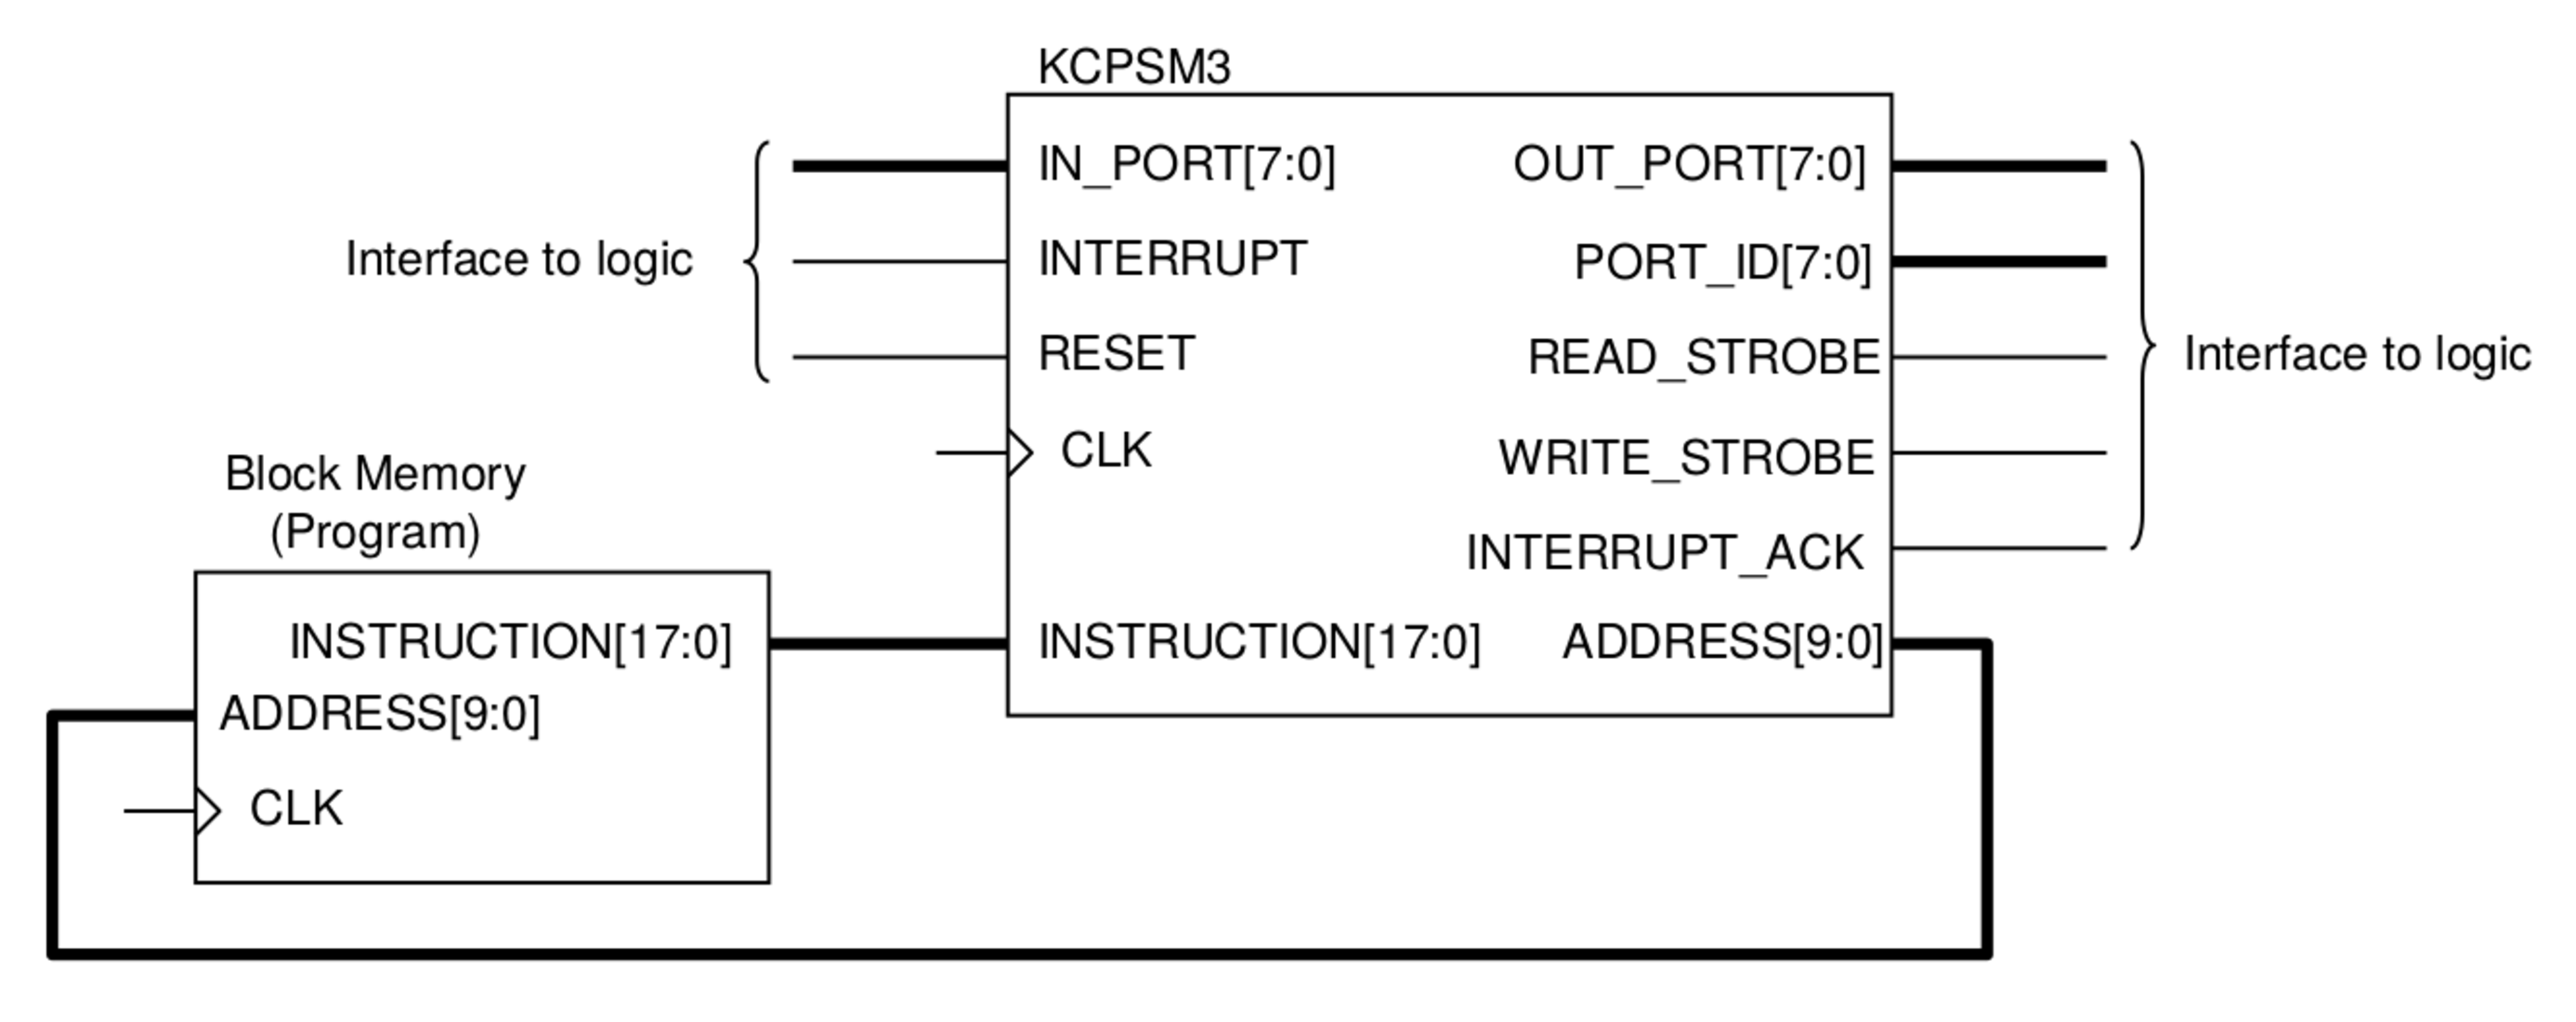
\includegraphics[height=0.60\textheight,width=0.85\textwidth]{kcpsm3}
%%  \end{block}
%%\end{frame}
%%
%%\begin{frame}
%%  \frametitle{Archivos relacionados a PicoBlaze dentro del firmware}
%%  \begin{block}{KCPSM3}
%%    \begin{itemize}
%%      \item kcpsm3.vhd
%%      \item uart\_tx.vhd
%%      \item uart\_rx.vhd
%%      \item kcuart\_tx.vhd
%%      \item kcuart\_rx.vhd
%%      \item bbfifo\_16x8.vhd
%%      \item GPSNFIFO.FMT
%%      \item HP\_LAGO.FMT
%%      \item GPS\_n\_fifo.vhd
%%      \item HP03\_par\_control.vhd
%%    \end{itemize}
%%\end{block}
%%\end{frame}
%
%\begin{frame}
%  \frametitle{Repasando el firmware}
%  \begin{block}{}
%    \centering
%    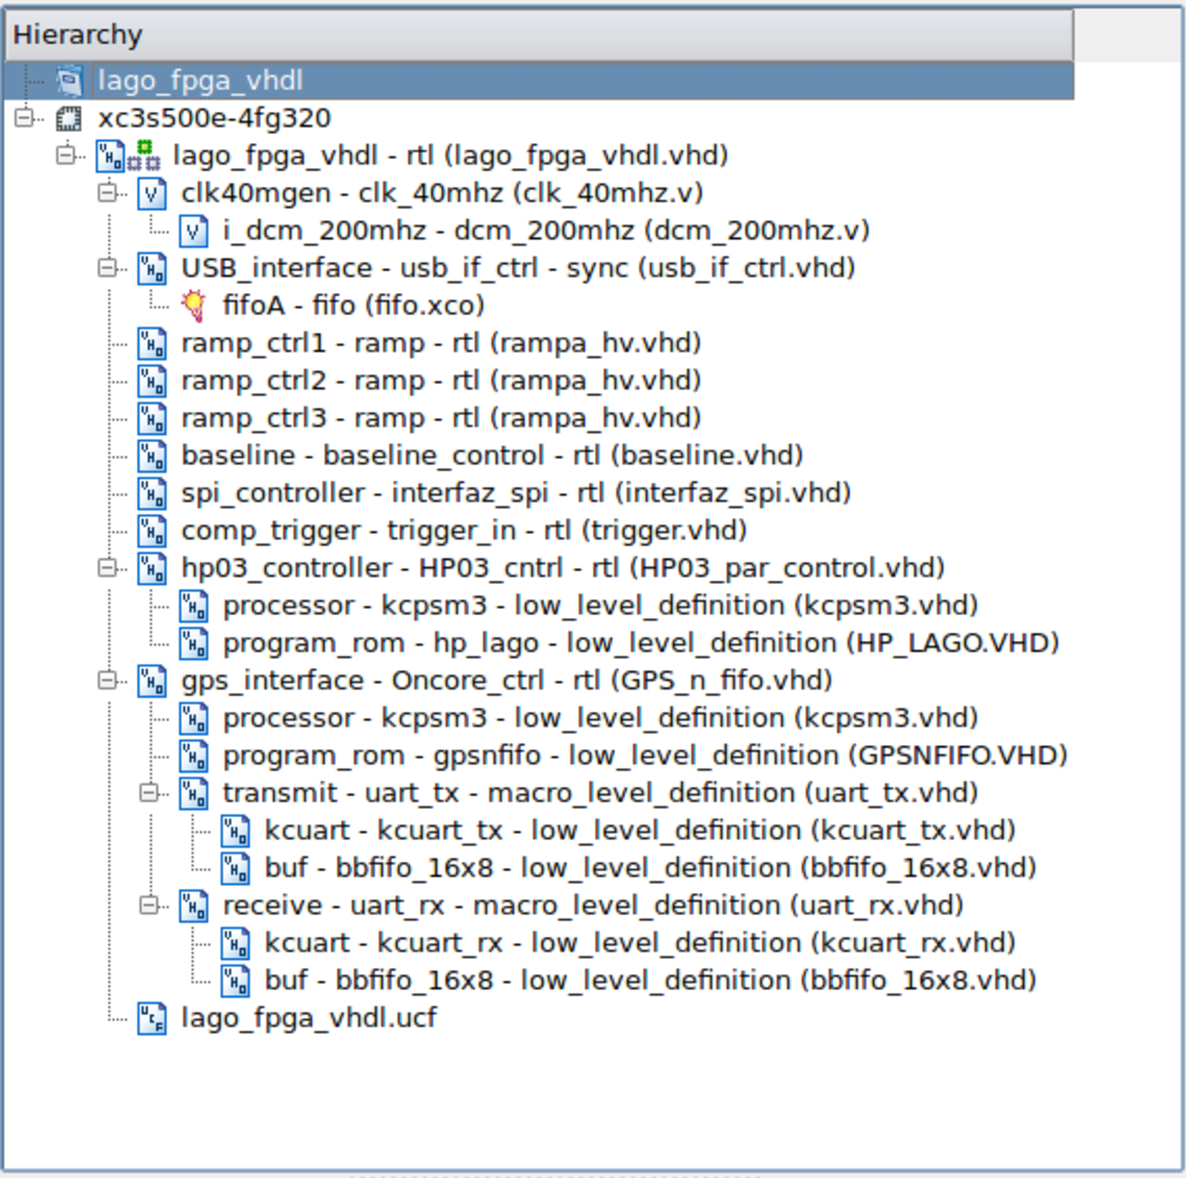
\includegraphics[height=0.75\textheight,width=0.75\textwidth]{jerarquia_lago}
%  \end{block}
%\end{frame}
%
%\begin{frame}
%  \frametitle{Repasando el firmware}
%  \begin{block}{En LAGO tenemos un Makefile que se ocupa de la mayoría de los
%                procesos complicados involucrados en generar el firmware para la
%                FPGA.}
%    \centering
%    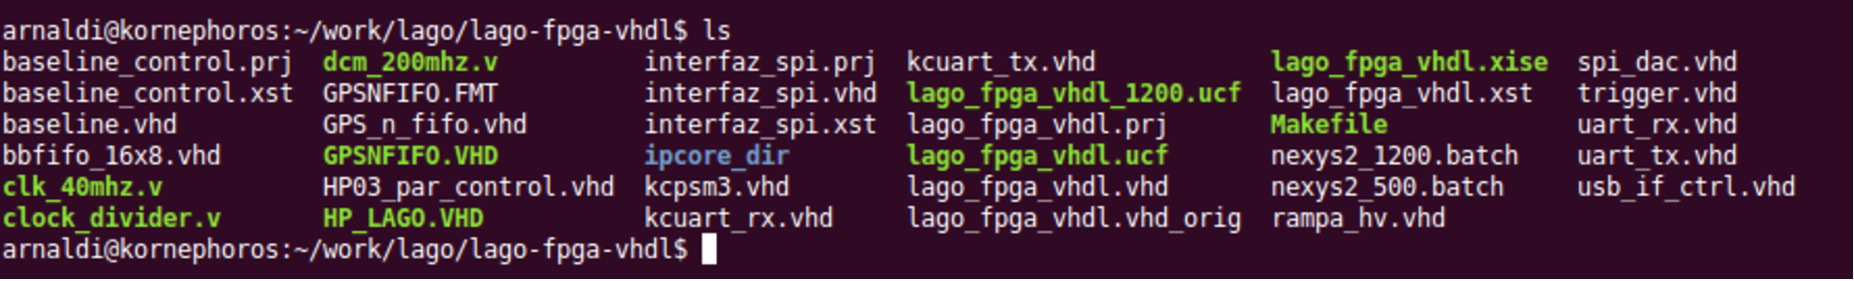
\includegraphics[height=0.30\textheight,width=\textwidth]{archivos_del_firmware}
%  \end{block}
%\end{frame}
%
%\begin{frame}
%  \frametitle{Repasando el firmware}
%    \begin{block}{¿Cuáles son los problemas a resolver en el futuro próximo?}
%      \begin{itemize}
%        \pause
%        \item La Nexys2 está obsoleta $\rightarrow$ hay que cambiar a una placa
%							alternativa 
%        \pause
%        \item Uno de los mayores problemas electrónicos que encontramos en el
%              trabajo diario está en el conector FX2 de Hirose $\rightarrow$ no
%							es confiable, falsos contactos, etc.
%        \pause
%        \item Hacer que los tres controladores de alta tensión sean idénticos
%							$\rightarrow$ actualmente hay dos manejados directamente por la
%							FPGA y uno que pasa a través del DAC.
%        \pause
%        \item Cambiar los módulos GPS y de PyT por algunos más actuales
%      \end{itemize}
%    \end{block}
%\end{frame}
%
%\subsection{La linea de base}
%\begin{frame}
%  \begin{center}
%    \Huge{\color{blue}{Las electrónicas: \\ La linea de base}}
%  \end{center}
%\end{frame}
%
%\subsubsection{¿Cuál el el problema a resolver?}
%
%\begin{frame}
%  \frametitle{Cambios aleatorios (o no tanto) en la linea de base}
%  \begin{block}{}
%    \centering
%    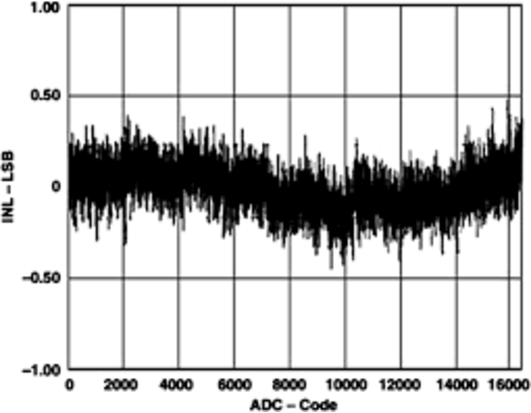
\includegraphics[height=0.55\textheight,width=0.75\textwidth]{shifting_baseline}
%  \end{block}
%\end{frame}
%
%\begin{frame}
%  \frametitle{Cambios aleatorios (o no tanto) en la linea de base}
%  \begin{block}{}
%    \centering
%    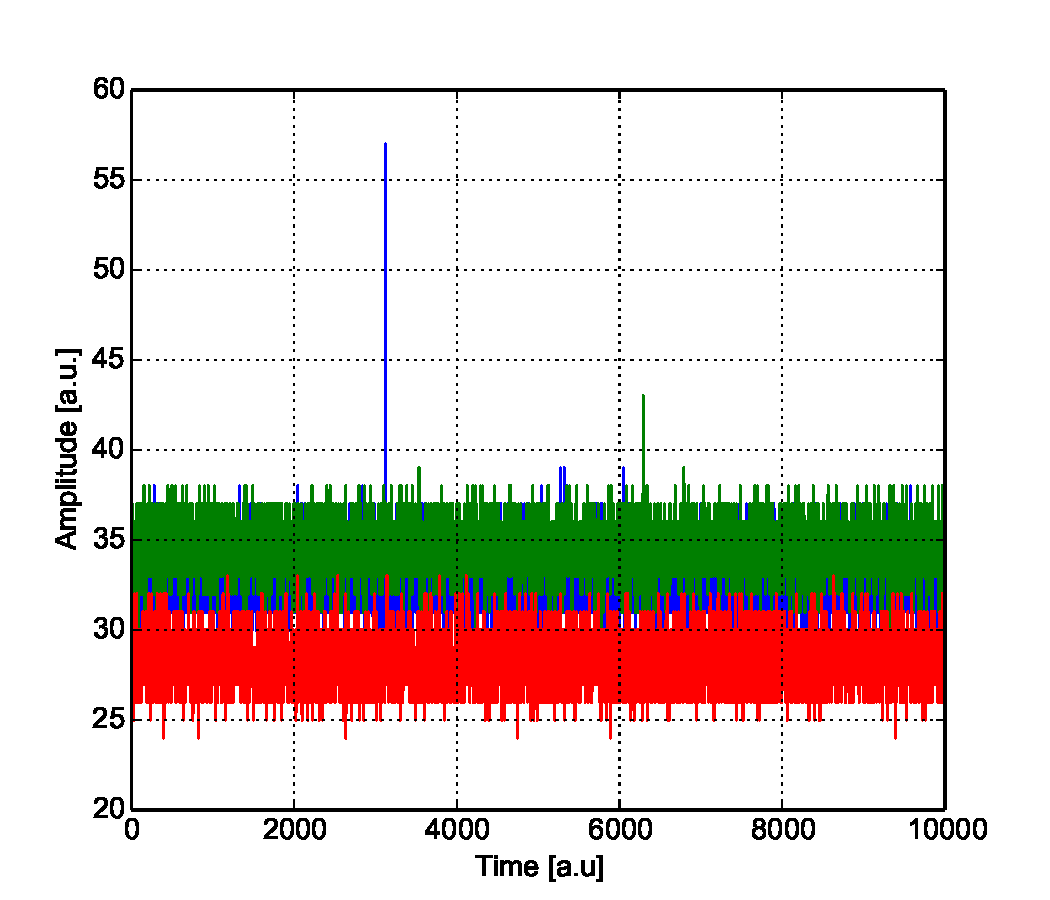
\includegraphics[height=0.55\textheight,width=0.75\textwidth]{tres_chann2}
%  \end{block}
%\end{frame}
%
%\begin{frame}
%  \frametitle{Cambios aleatorios (o no tanto) en la linea de base}
%  \begin{block}{}
%    \centering
%    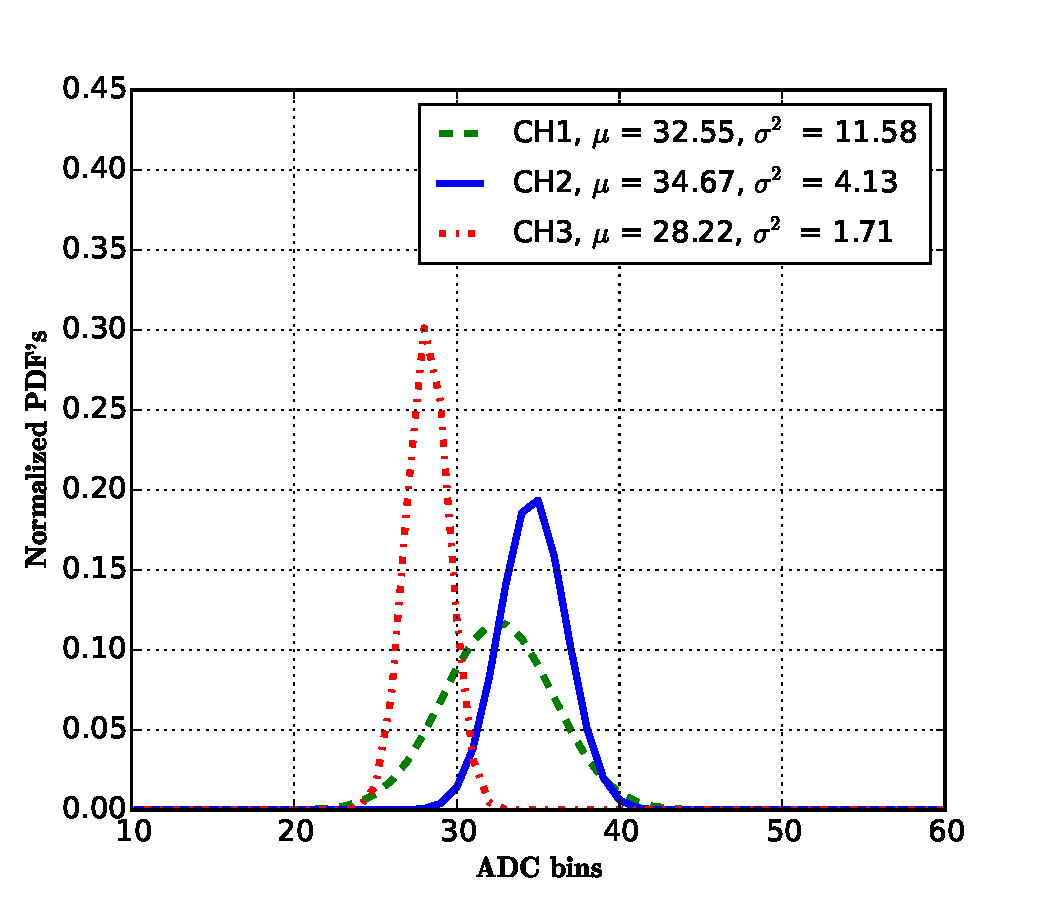
\includegraphics[height=0.55\textheight,width=0.75\textwidth]{histogramas_por_canal_fija}
%  \end{block}
%\end{frame}
%
%\begin{frame}
%  \frametitle{Cambios lentos y/o rápidos en la linea de base}
%    \begin{block}{}
%      \begin{itemize}
%        \pause
%        \item Ruido excesivo debido a transitorios ($>$ 2 ms)
%        \pause
%        \item Cambios debidos a temperatura (drifts térmicos, aging, etc.
%              principalmente en los componentes electrónicos activos)
%        \pause
%        \item ¿Qué es eso de 50 ADC?: Como trabajamos con ADCs de 10 bits, la
%              tensión mínima detectable es de 976\,$\mu$V y se coloca un offset de
%              50 ADC, es decir, $\sim$49\,mV (para una referencia de 1\,V en el
%              ADC, que es la configuración normal de nuestra toma de datos).
%%        \item Mostrar las formulas de conversión ADC, 10 bits, etc
%%       \pause
%%        \item Uniformizar el formato de los datos/archivos guardados
%%       \pause
%      \end{itemize}
%    \end{block}
%\end{frame}
%
%\subsubsection{La solución: hardware}
%
%\begin{frame}
%  \frametitle{La placa de adquisición de LAGO}
%  \begin{block}{}
%    \centering
%    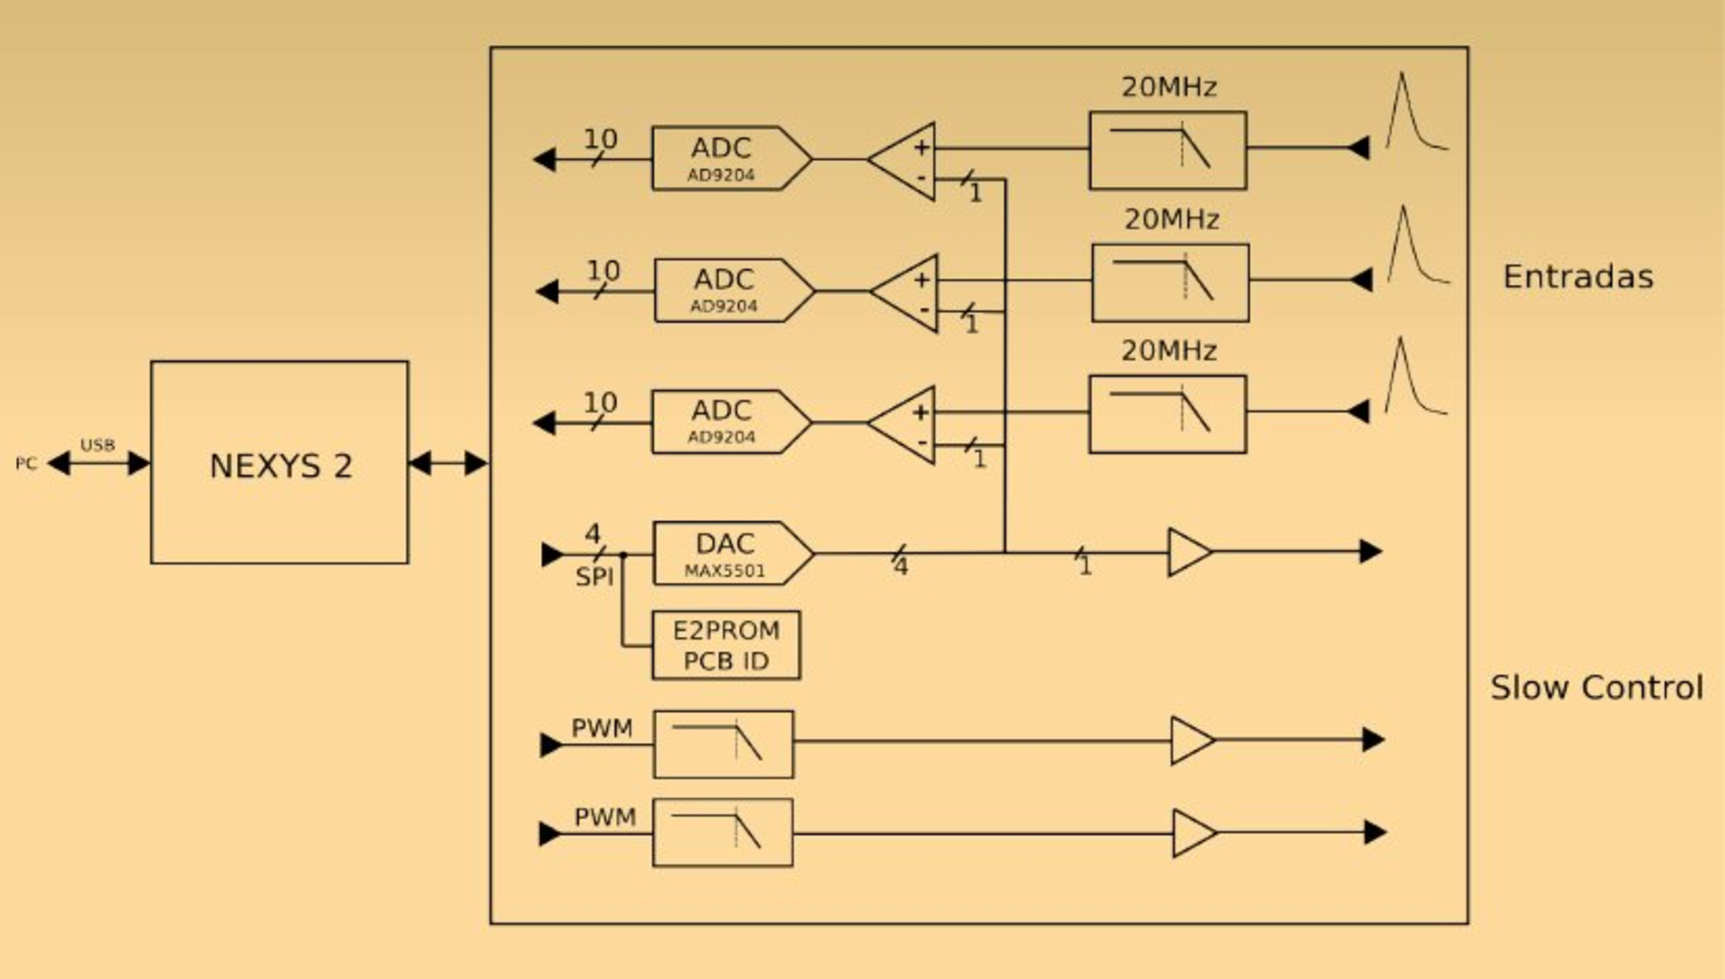
\includegraphics[height=0.55\textheight,width=0.75\textwidth]{diagrama_en_bloques_lago}
%  \end{block}
%\end{frame}
%
%\begin{frame}
%  \frametitle{El front-end}
%  \begin{block}{}
%    \centering
%    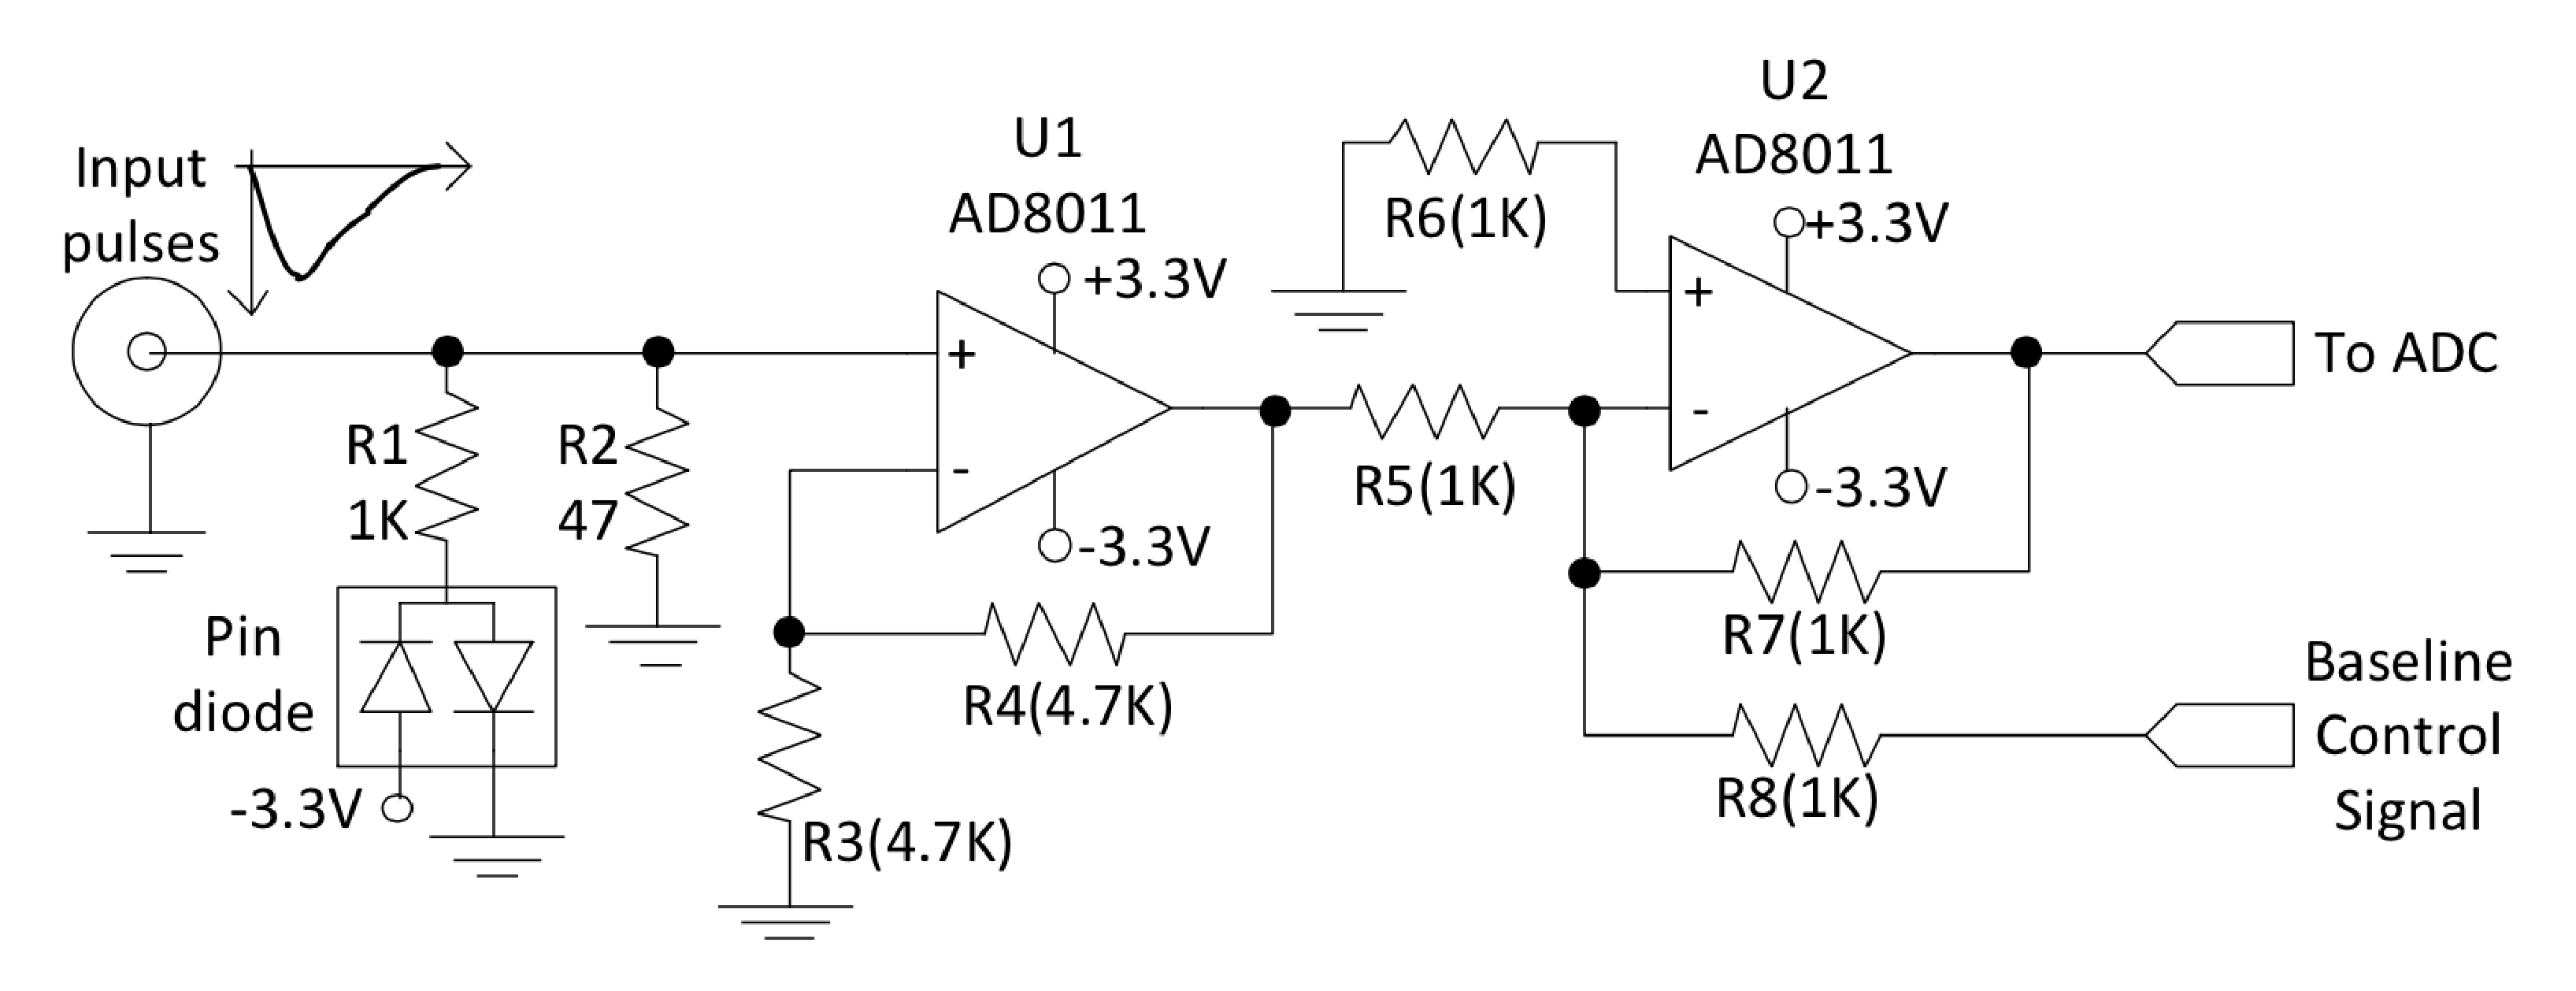
\includegraphics[height=0.50\textheight,width=0.75\textwidth]{front_end_circuit2}
%  \end{block}
%\end{frame}
%
%\begin{frame}
%  \frametitle{El front-end}
%  \begin{block}{}
%    \centering
%    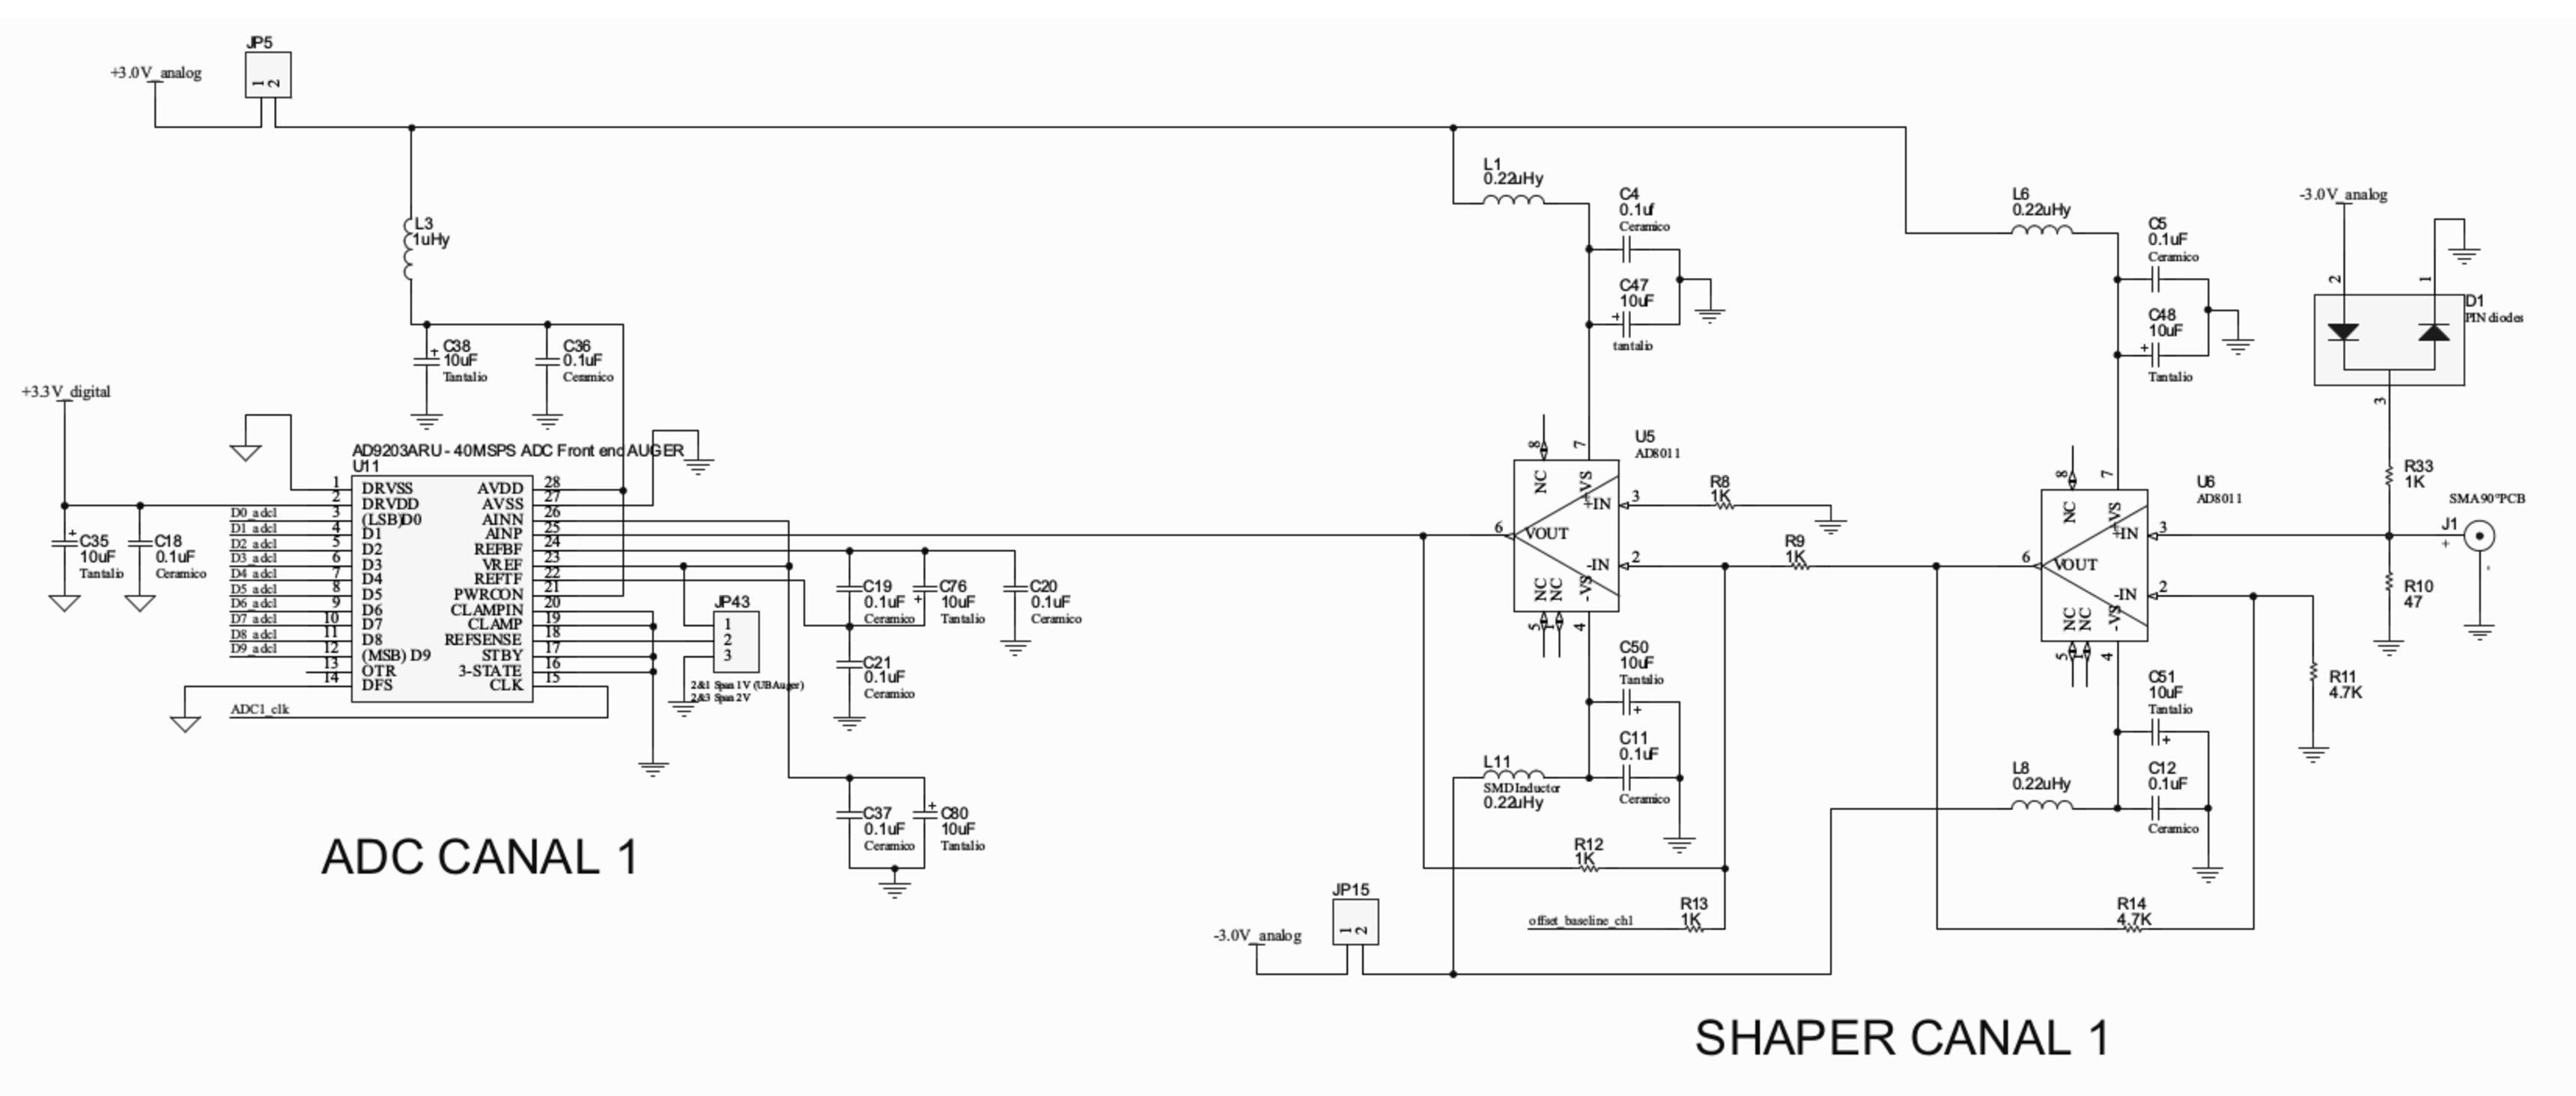
\includegraphics[height=0.75\textheight,width=0.95\textwidth]{shaper_lago}
%  \end{block}
%\end{frame}
%
%\subsubsection{La solución: software}
%\begin{frame}
%  \frametitle{FPGA: baseline.vhd}
%  \begin{block}{}
%    \centering
%    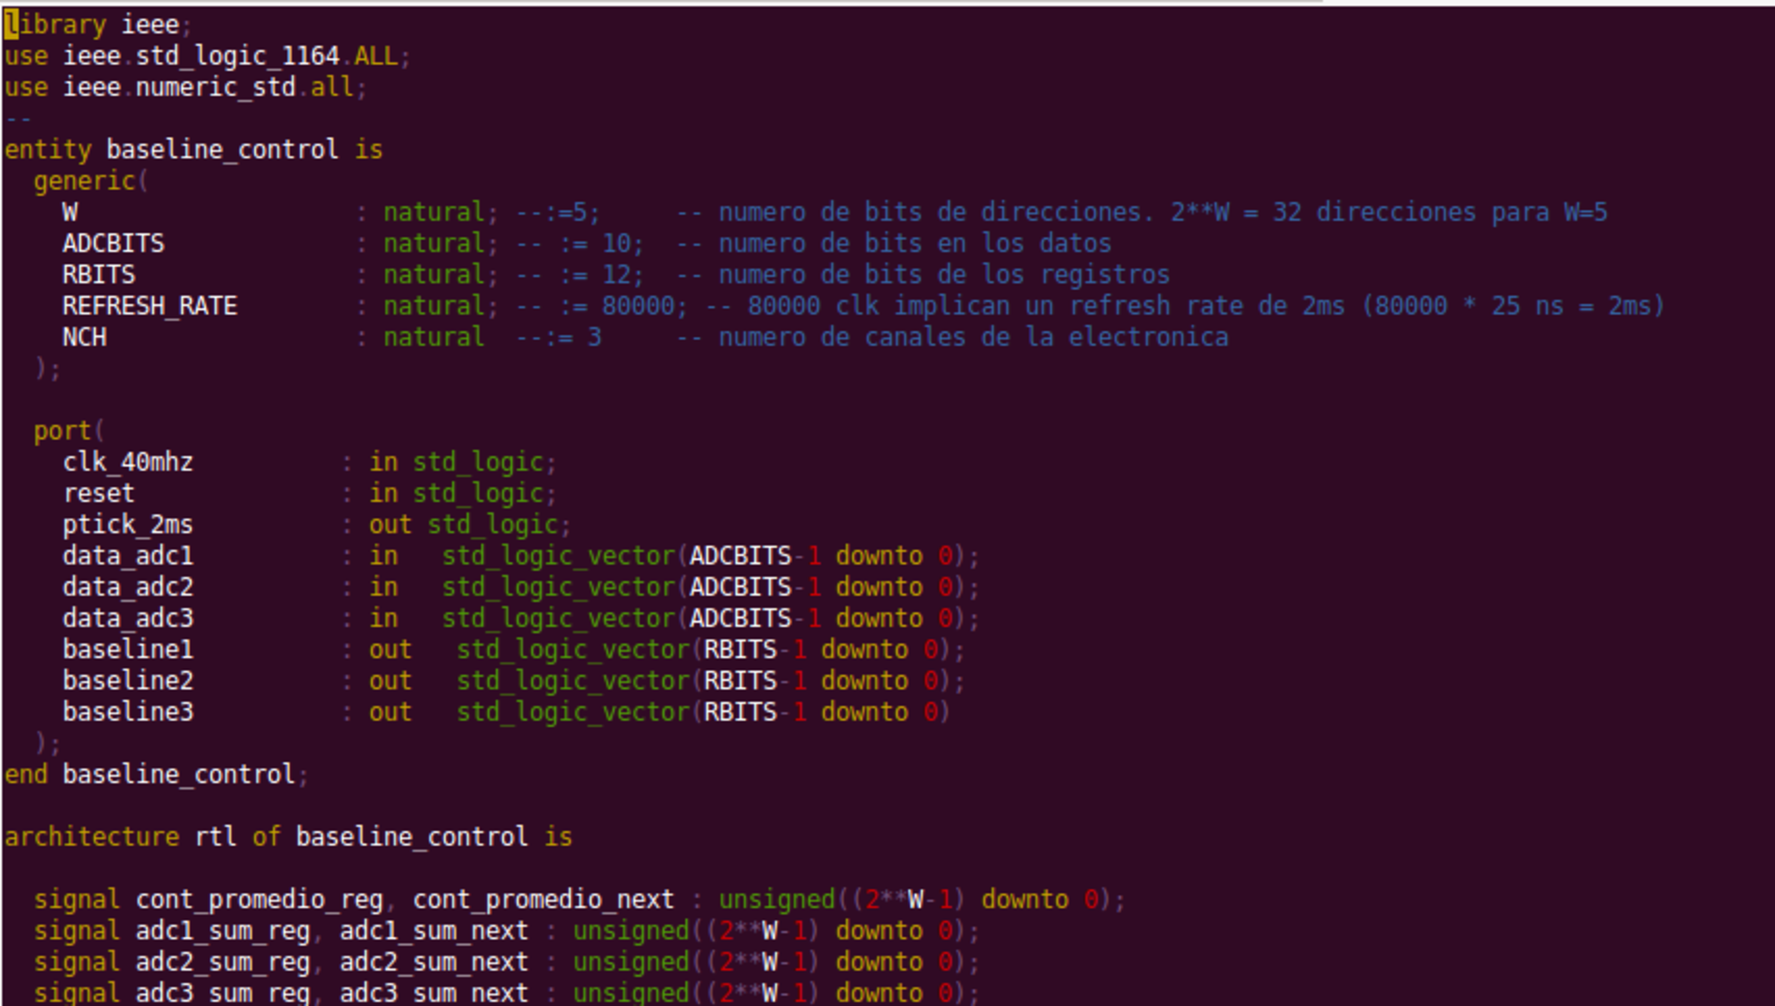
\includegraphics[height=0.55\textheight,width=0.75\textwidth]{baseline_vhd}
%  \end{block}
%\end{frame}
%
%\begin{frame}
%  \frametitle{FPGA: baseline.vhd}
%  \begin{block}{}
%    \centering
%    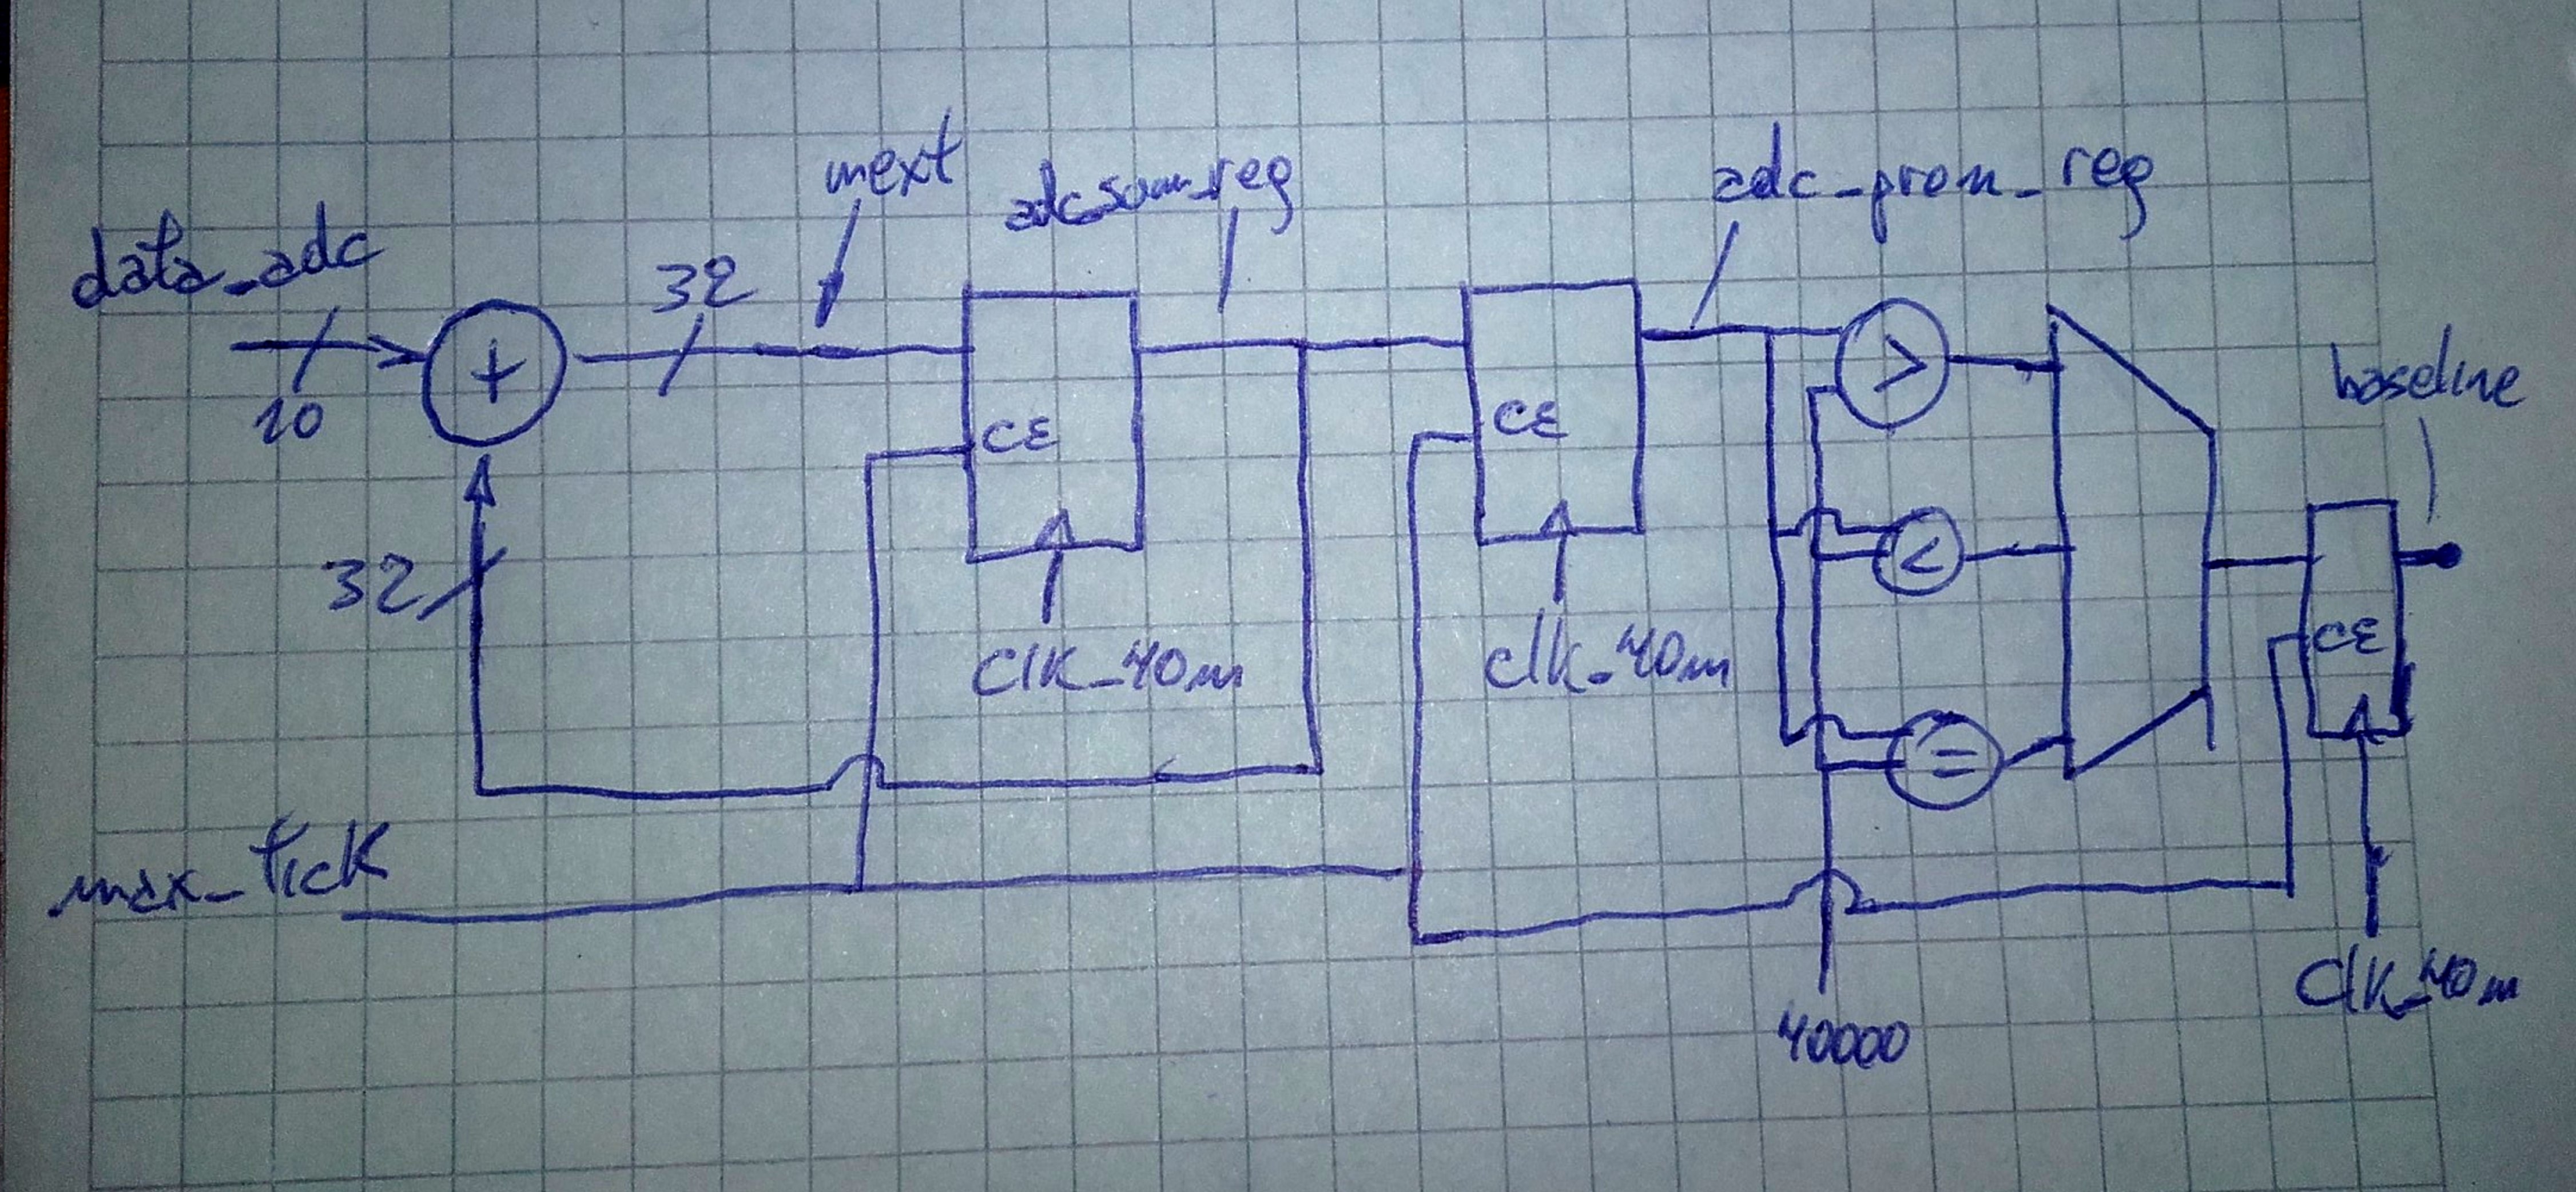
\includegraphics[height=0.60\textheight,width=0.75\textwidth]{ma_filter_lago2}
%  \end{block}
%\end{frame}
%
%\begin{frame}
%  \frametitle{FPGA: resultado}
%  \begin{block}{}
%    \centering
%    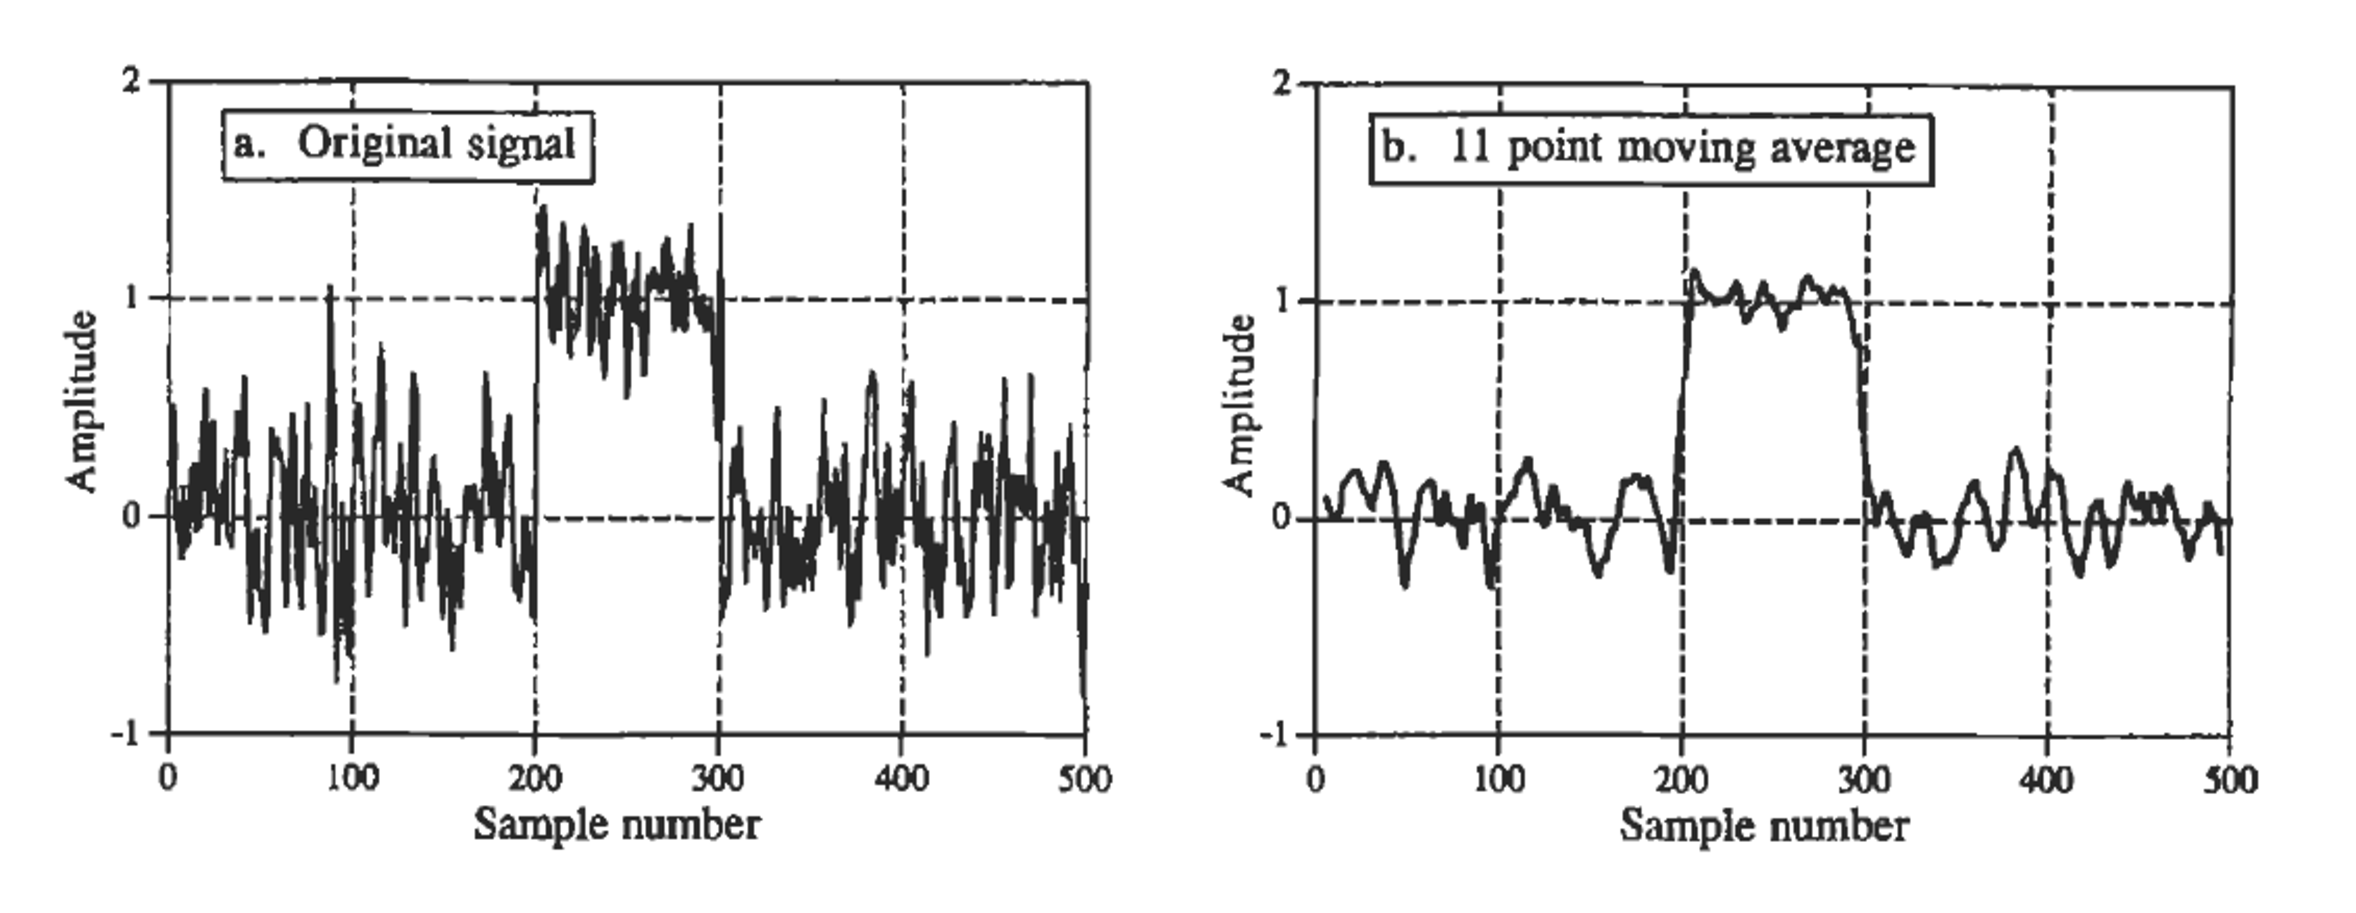
\includegraphics[height=0.50\textheight,width=0.75\textwidth]{resultado_ma_filter_ej}
%  \end{block}
%\end{frame}
%
%\begin{frame}
%  \frametitle{FPGA: resultado}
%  \begin{block}{}
%    \centering
%    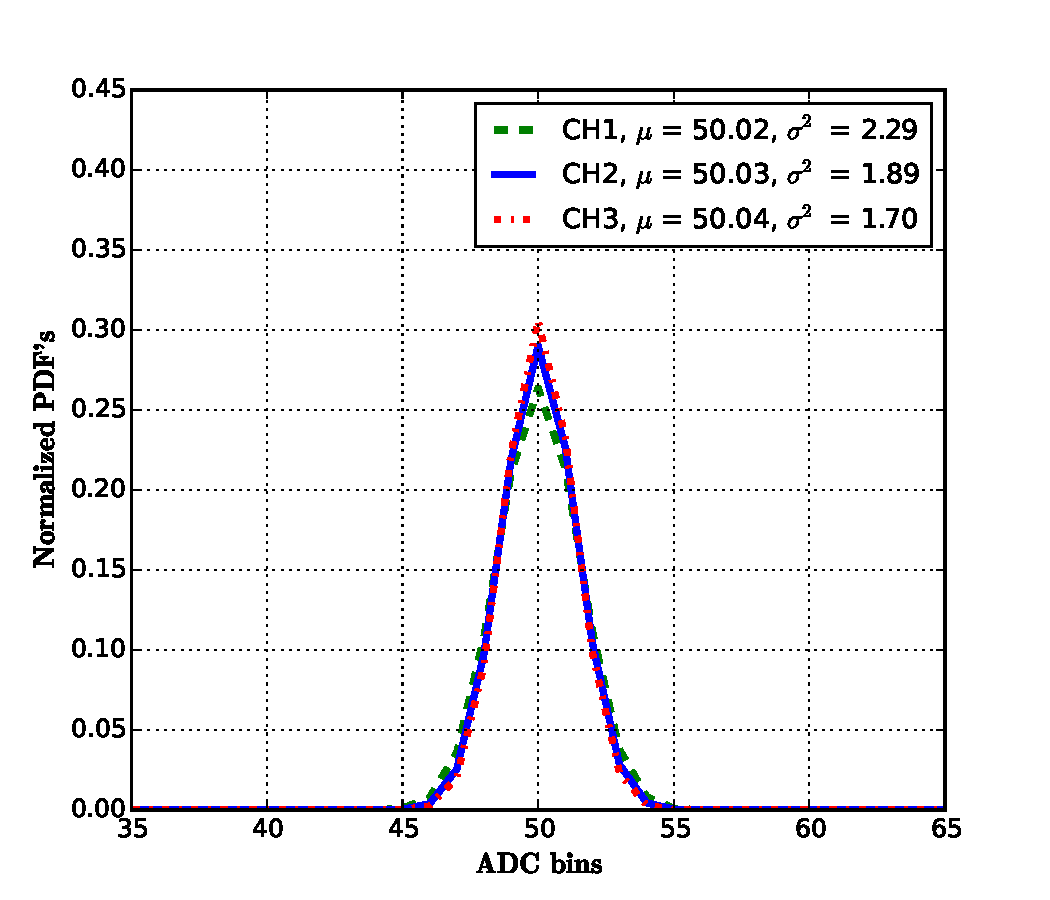
\includegraphics[height=0.55\textheight,width=0.75\textwidth]{histogramas_por_canal_normal}
%  \end{block}
%\end{frame}
%
%\begin{frame}
%  \frametitle{FPGA: resultado}
%	\begin{columns}
%	\begin{column}{0.50\textwidth}
%  \begin{block}{}
%    \begin{center}
%    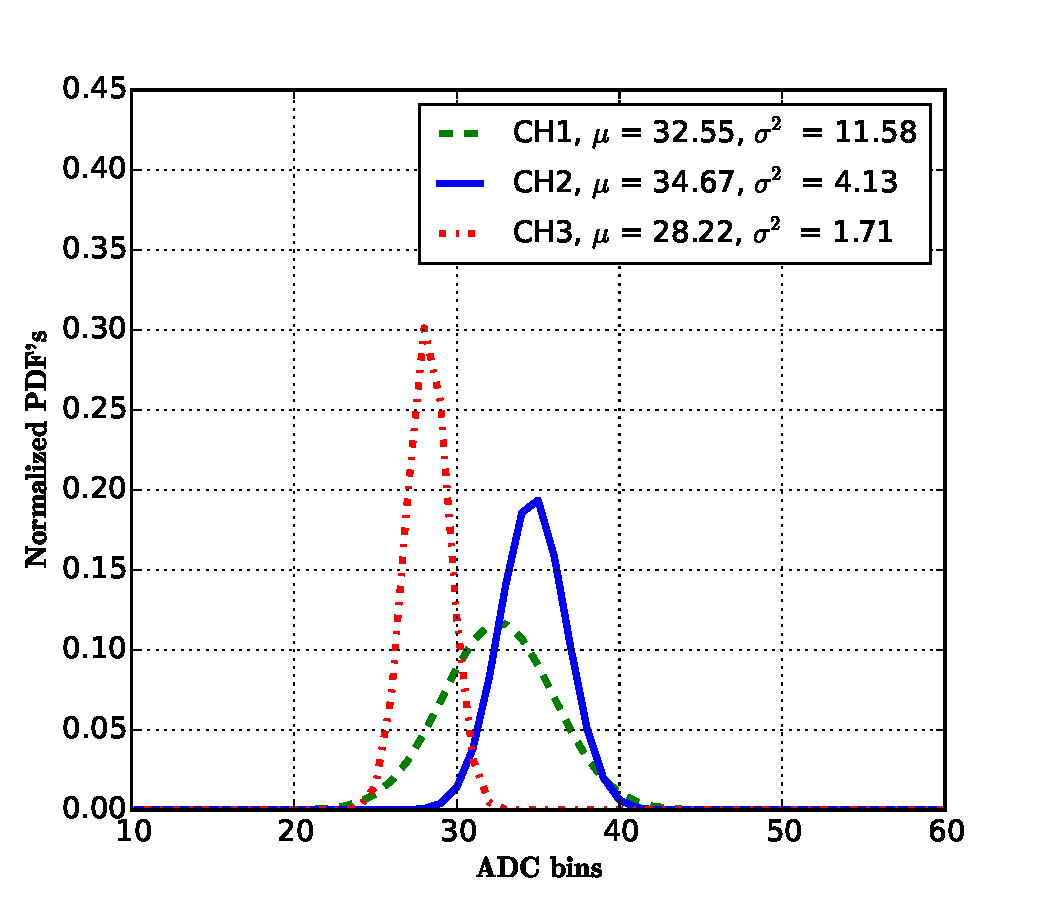
\includegraphics[width=\textwidth]{histogramas_por_canal_fija}
%    \end{center}
%  \end{block}
%	\end{column}
%	\begin{column}{0.50\textwidth}
%  \begin{block}{}
%    \begin{center}
%    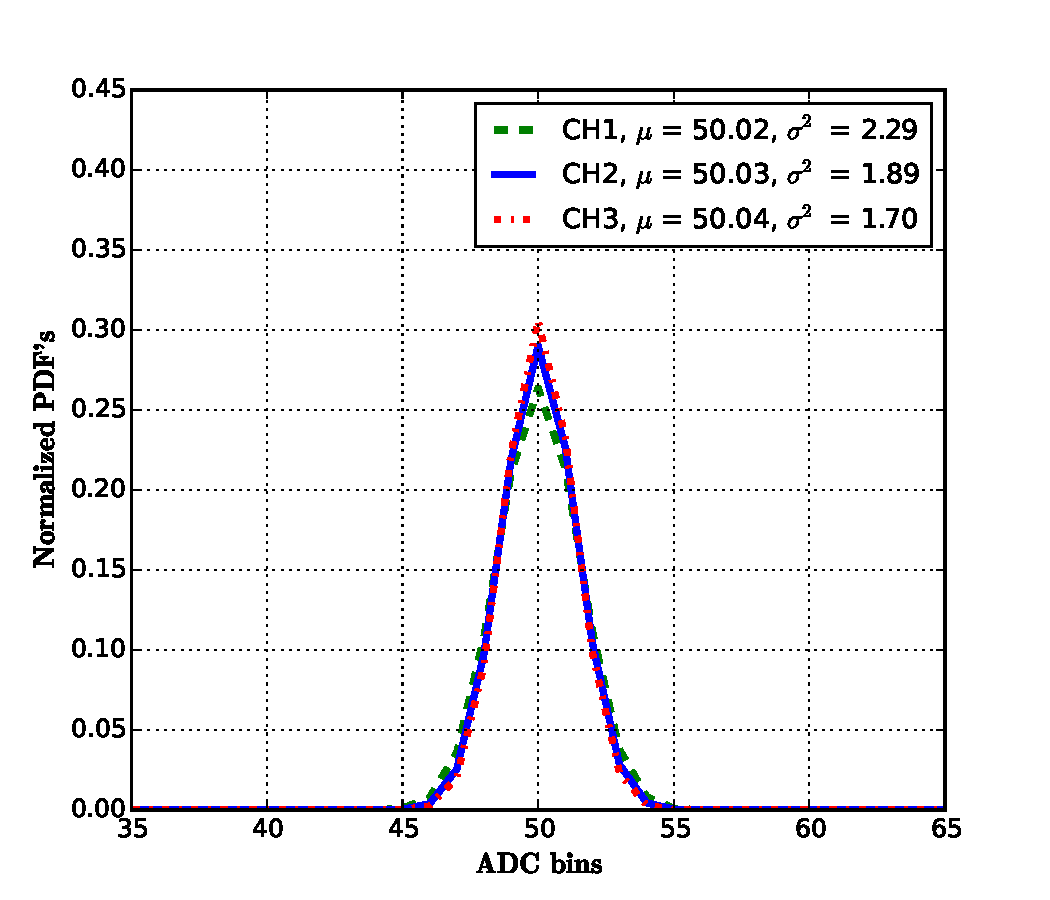
\includegraphics[width=\textwidth]{histogramas_por_canal_normal}
%    \end{center}
%  \end{block}
%	\end{column}
%  \end{columns}
%\end{frame}
%
%\subsection{Instrumentación de cuatro canales}
%\begin{frame}
%  \begin{center}
%    \Huge{\color{blue}{Las electrónicas: \\ Placa de adquisición de cuatro canales}}
%  \end{center}
%\end{frame}
%
%\begin{frame}
%	\frametitle{Hardware}
%		\begin{exampleblock}{Características}
%			\begin{itemize}
%				\item Cuatro \alert{entradas diferenciales}, conectores tipo
%							\alert{LEMO}
%				\item Un convertidor ADC \alert{AD9216} dual de hasta \alert{100\,MS/s},
%							rango dinámico de conversión de +1\,V a -1\,V
%				\item Reloj configurable para los ADC (permite cambiar la frecuencia de
%							muestreo)
%				\item Está basado en el microcontrolador \alert{MicroBlaze} de Xilinx
%			\end{itemize}
%		\end{exampleblock}
%\end{frame}
%
%\begin{frame}
%	\frametitle{Hardware}
%		\begin{exampleblock}{Características (Cont.)}
%			\begin{itemize}
%				\item Buses de datos de 10\,bits
%				\item Amplificadores diferenciales \alert{AD8138} (mejora en ruido)
%				\item Conectividad a la Nexys2 a través del conector HIROSE FX2-100P
%				\item Usa los recursos de la tarjeta \alert{Nexys2-500E} para la
%							implementación de la arquitectura y la comunicación con la PC.
%				\item Desarrollo de la Universidad Autónoma de Puebla (Rubén
%							Conde)
%			\end{itemize}
%		\end{exampleblock}
%\end{frame}
%
%\begin{frame}
%	\frametitle{Hardware}
%		\begin{exampleblock}{Características (Cont.)}
%			\begin{itemize}
%				\item Se puede evitar la \underline{\textit{sobre}} y
%							\underline{\textit{sub}} saturación de la señal actuando
%							sobre un pin dedicado del amplificador AD8138. Provee entonces
%							\alert{ajuste dinámico del offset} de la señal de entrada.
%				\item Utiliza el puerto RS232 para el envío de información a la PC, esto
%							implica velocidades de transmisión de datos limitadas.
%				\item No tiene electrónica dedicada para alimentar/polarizar los PMT
%			\end{itemize}
%		\end{exampleblock}
%\end{frame}
%
%\begin{frame}
%  \frametitle{El sistema de 4 canales}
%  \begin{block}{}
%    \begin{center}
%    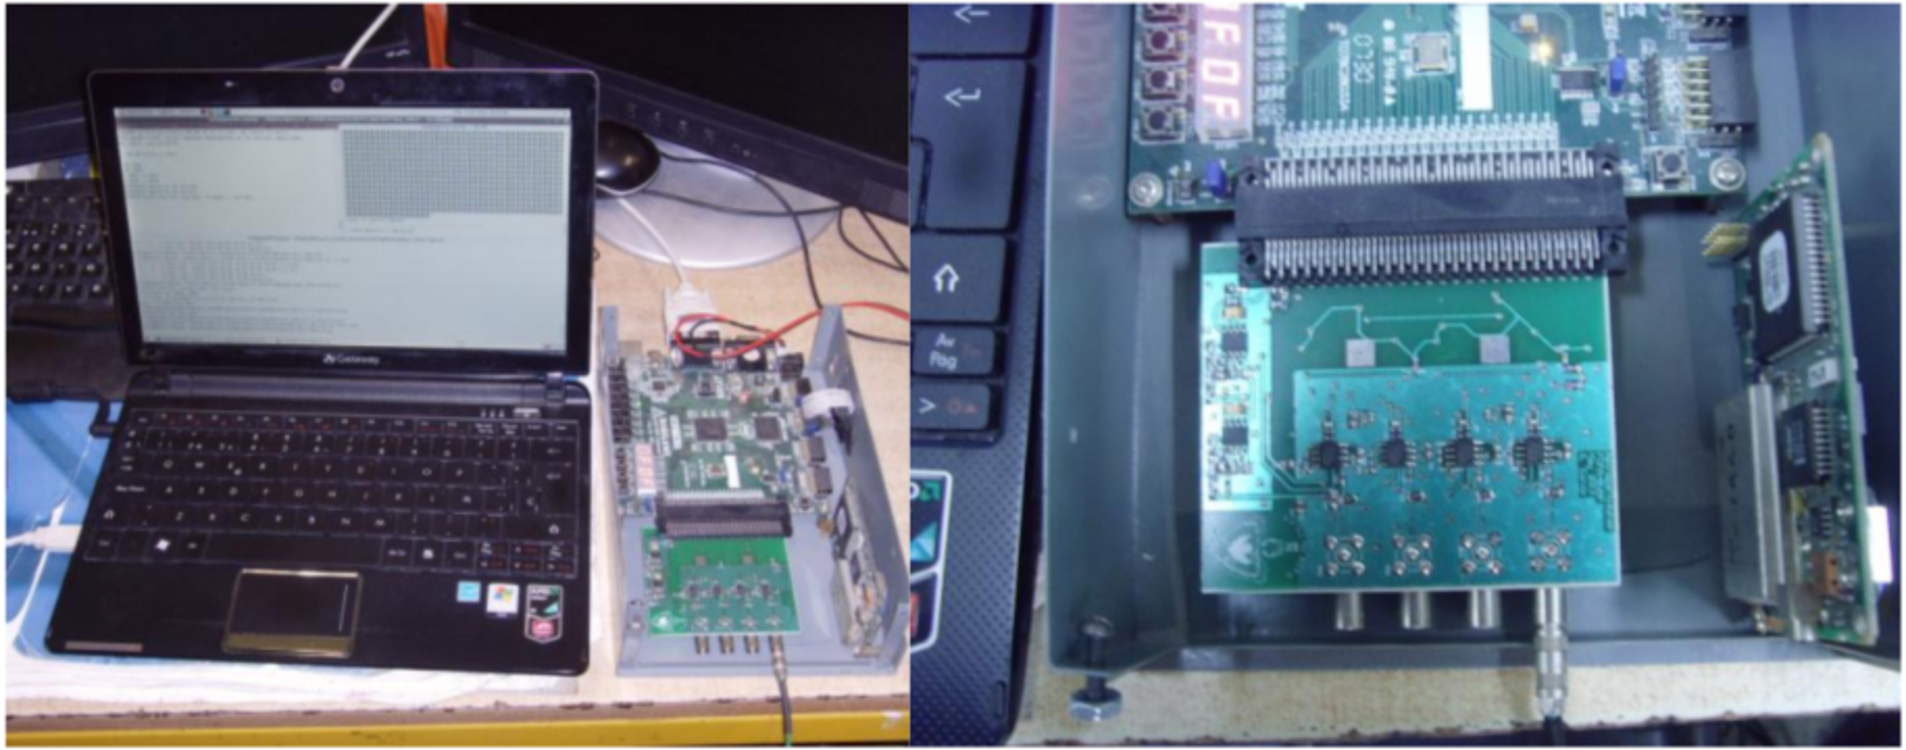
\includegraphics[height=0.55\textheight,width=0.98\textwidth]{vista_sistema_lago_mx}
%		\end{center}
%  \end{block}
%\end{frame}
%
%\begin{frame}
%  \frametitle{Hardware de 4 canales: bloques}
%  \begin{block}{}
%    \begin{center}
%    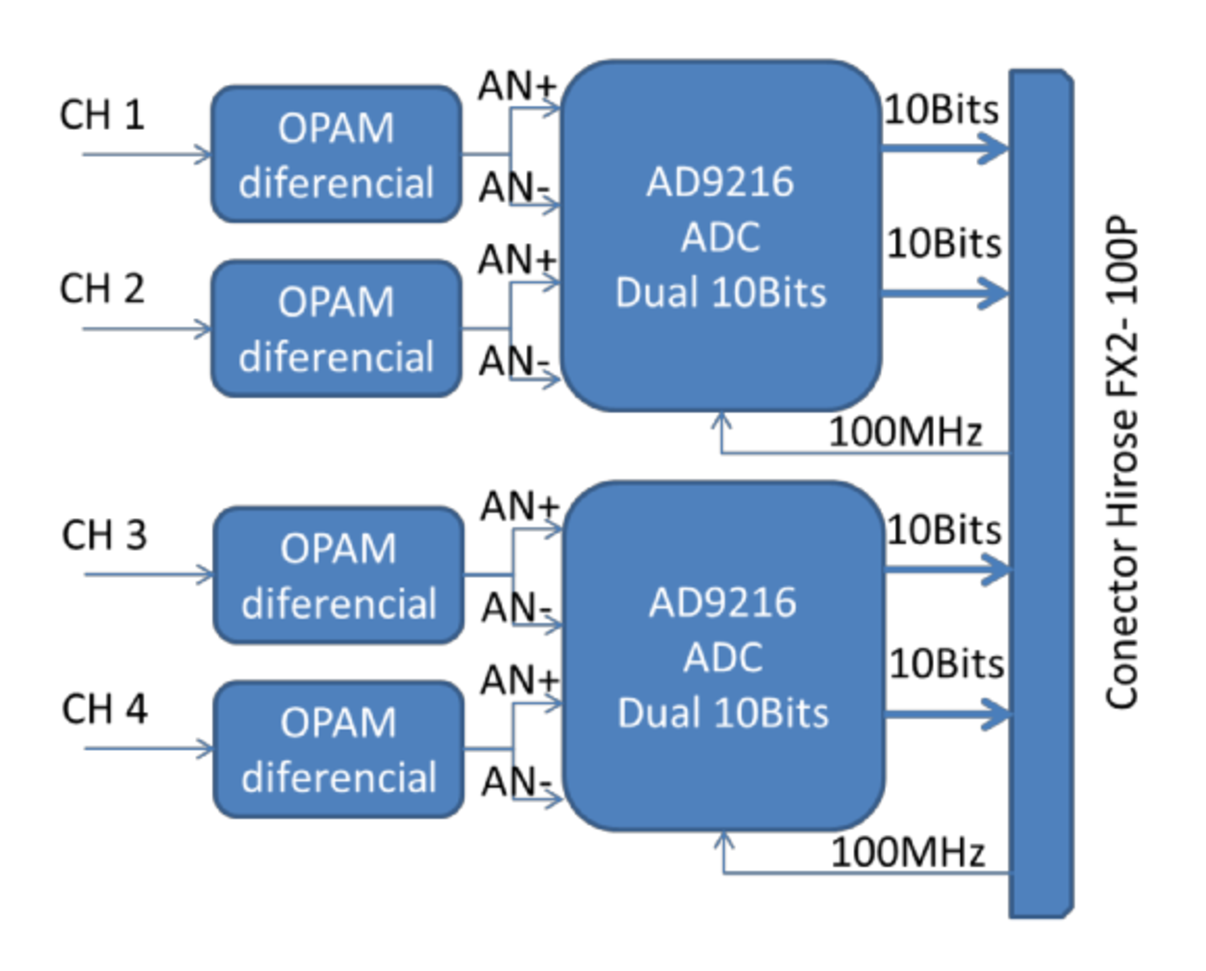
\includegraphics[height=0.75\textheight,width=0.75\textwidth]{bloques_lago_mx}
%		\end{center}
%  \end{block}
%\end{frame}
%
%\begin{frame}
%  \frametitle{Hardware de 4 canales: interfaz diferencial}
%  \begin{block}{}
%    \begin{center}
%    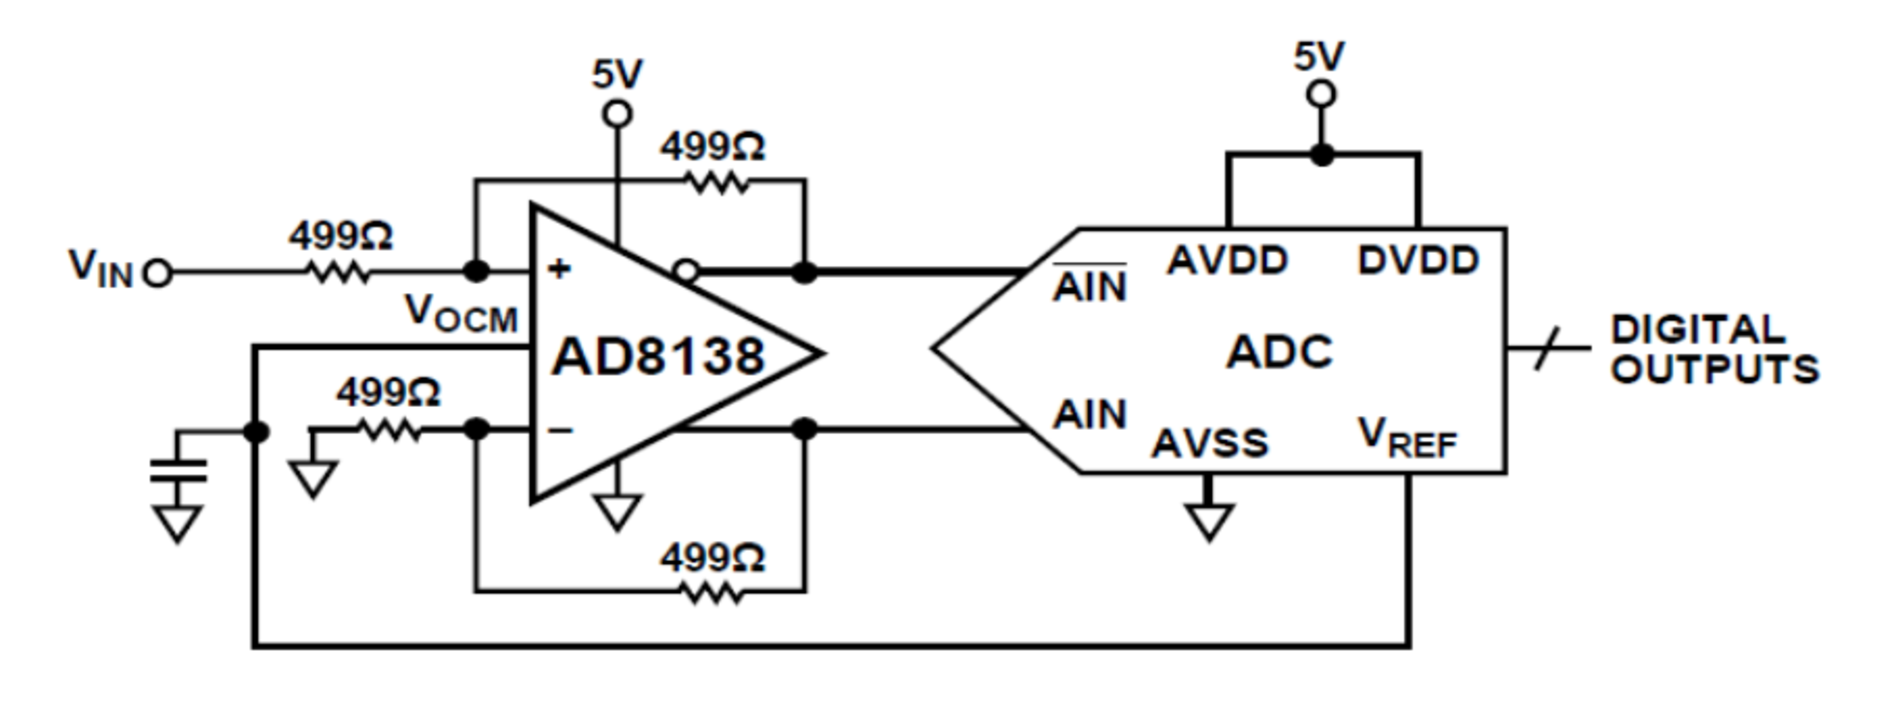
\includegraphics[height=0.50\textheight,width=0.75\textwidth]{configuracion_diferencial_lago_mx}
%		\end{center}
%  \end{block}
%\end{frame}
%
%\begin{frame}
%	\frametitle{Software}
%		\begin{exampleblock}{Características}
%			\begin{itemize}
%				\item Se han desarrollado scripts (\alert{Bash} y \alert{Perl}) que
%							ejecutan diferentes etapas del
%							proceso de adquisición de datos.
%				\item El sistema completo está basado en el sistema de configuración de
%							umbrales utilizado en Auger
%				\item Scripts:
%							\begin{itemize}
%								\item ejecuta.sh
%								\item umbral.sh
%								\item traza.sh
%								\item rate.sh
%							\end{itemize}
%			\end{itemize}
%		\end{exampleblock}
%\end{frame}


%\begin{frame}
%	\frametitle{¿Qué es LAGO?}
%	\framesubtitle{\textit{Large Aperture Gamma Ray Burst Observatory}}
%
%\begin{columns}
%	\begin{column}{0.40\textwidth}
%		\begin{block}{Varios sitios (\textgreater4000msnm)}
%    	\begin{itemize}[<+->]
%      	\item  México (Cerro La Negra)
%      	\item  Bolivia (Chacaltaya)
%      	\item  Venezuela (Mérida)
%				\item  Argentina (Auger)
%				\item	 Ecuador (Chimborazo)
%    	\end{itemize}
%		\end{block}
%	\end{column} 
% 	\begin{column}{0.55\textwidth}
%  	\includegraphics[width=\textwidth]{../media/sitios_lago.jpg}
% \end{column}
%\end{columns}
%\end{frame} 
%
%\begin{frame}
%	\frametitle{Detectores Cherenkov}
%	\framesubtitle{PMT}
%\begin{columns}
%	\begin{column}{0.50\textwidth}
%  	\fbox{\includegraphics[width=\textwidth]{../media/pmt_otro_inet.jpg}}
%	\end{column} 
% 	\begin{column}{0.50\textwidth}
%  	\fbox{\includegraphics[width=0.7\textwidth]{../media/divisor_pmt.jpg}}
% \end{column}
%\end{columns}
%\end{frame} 
%
%\begin{frame}
%	\frametitle{Detectores Cherenkov}
%	\framesubtitle{PMT}
%\begin{columns}
%	\begin{column}{0.50\textwidth}
%  	\fbox{\includegraphics[width=0.8\textwidth]{../media/nahuelito.jpg}}
%	\end{column} 
% 	\begin{column}{0.50\textwidth}
%  	\fbox{\includegraphics[width=\textwidth]{../media/fototubo_pmt.jpg}}
% \end{column}
%\end{columns}
%\end{frame} 
%
%\section[Lo que teníamos]{¿Qué teníamos hasta ahora?}
%\begin{frame}
%	\frametitle{¿Qué teníamos hasta ahora?}
%
%\begin{columns}
%	\begin{column}{0.40\textwidth}
%		\begin{block}{Electrónica dedicada para Auger}
%    	\begin{itemize}[<+->]
%      	\item Poco flexible 
%      	\item Información limitada
%      	\item Número limitado de UB 
%				\item Comunicación de datos por puerto serie
%				\item	Tiempos de adquisición largos
%				\item	Poco volumen de almacenamiento
%				\item Sin control línea de base	
%    	\end{itemize}
%		\end{block}
%	\end{column} 
% 	\begin{column}{0.55\textwidth}
%  	\fbox{\includegraphics[width=\textwidth]{../media/electronica_auger.jpg}}
% \end{column}
%\end{columns}
%\end{frame} 
%
%
%
%\section{¿Cómo se logró?}
%
%\begin{frame}
%	\frametitle{Placa de digitalización}
%\begin{columns}
%	\begin{column}{0.40\textwidth}
%		\begin{block}{Características}
%    	\begin{itemize}[<+->]
%      	\item 3 canales
%      	\item ADC de 10 bits
%      	\item 40 MSPS 
%				\item Pulse shaper
%				\item Control activo de la línea de base
%				\item Control de alta tensión para base de PMT
%    	\end{itemize}
%		\end{block}
%	\end{column} 
% 	\begin{column}{0.55\textwidth}
%  	\only<1-3>{\fbox{\includegraphics[width=0.7\textwidth]{../media/placa_lago.jpg}}}
%  	\only<4-6>{\fbox{\includegraphics[width=\textwidth]{../media/newel_frente.jpg}}}
% \end{column}
%\end{columns}
%\end{frame} 
%
%\begin{frame}
%	\frametitle{Diagrama en bloques}
%	\begin{block}{}
%  	\includegraphics[width=\textwidth]{../media/diagrama_en_bloques_lago.jpg}
%	\end{block}
%\end{frame} 
%
%\begin{frame}
%	\frametitle{Front-end}
%	\begin{block}{}
%  	\includegraphics[width=\textwidth]{../media/front_end_lago.jpg}
%	\end{block}
%\end{frame} 
%
%\begin{frame}
%	\frametitle{Bloques en la FPGA}
%%	\begin{block}{}
%	\begin{center}
%  	\fbox{\includegraphics[width=0.8\textwidth]{../media/bloques_fpga_lago}}
%	\end{center}
%%	\end{block}
%\end{frame} 
%
%\begin{frame}
%	\frametitle{Estándares implementados en la FPGA}
%		\begin{block}{}
%    	\begin{itemize}
%      	\item Interfaz SPI para el control de la línea 
%							de base del sistema a través de un DAC 
%      	\item Interfaz I2C para la obtención de los 
%							datos del sensor de presión y temperatura
%      	\item Interfaz RS232 para la comunicación 
%							bidireccional con el receptor GPS
%      	\item Interfaz USB bidireccional para la 
%							comunicación de datos y el envío de 
%							órdenes desde la PC
%    	\end{itemize}
%		\end{block}
%\end{frame} 
%
%\begin{frame}
%	\frametitle{Facilidades del código desarrollado}
%		\begin{block}{Datos}
%    	\begin{itemize}
%      	\item GPS
%    		\begin{itemize}
% 					\item Tiempo en formato UTC o GPS
%    		\end{itemize}
%      	\item Presión y temperatura
%      	\item 3 canales
%      	\item Contador de triggers
%      	\item Se puede determinar el canal que tuvo un 
%							evento de trigger
%      	\item Monitoreo constante del reloj del sistema
%    	\end{itemize}
%		\end{block}
%\end{frame} 
%
%\begin{frame}
%	\frametitle{Interfaz USB}
%		\begin{block}{Características}
%    	\begin{itemize}
%      	\item Bus de datos bidireccional de 8 bits
% 				\item 6 líneas de control (handshaking)
%      	\item Transferencia sincrónica de datos
%      	\item Velocidad de transferencia de datos en 
%							torno a los 25 MB/s
%      	\item Utilización de librerías open source LGPL
%      	\item Implementado sobre un firmware propio, 
%							pero sin borrar el firmware que trae la 
%							Nexys2
%    	\end{itemize}
%		\end{block}
%\end{frame} 
%
%\begin{frame}
%	\frametitle{Soluciones: El software}
%		\begin{block}{Lago.cpp}
%    	\begin{itemize}
%      	\item Un sólo software para manejar todas las 
%							funciones implementadas en la FPGA
% 				\item Capacidad de consultar y configurar 
%							registros de forma independiente
%      	\item Control separado de cada canal
%      	\item Adquisición de datos por puerto USB 
%      	\item Rate de pulsos de 10 kHz para el modo
%							trigger normal y $\approx$ 100 kHz para el modo
%							subtrigger
%    	\end{itemize}
%		\end{block}
%\end{frame} 
%
%\begin{frame}
%\begin{block}{Pruebas: un ejemplo de análisis online}
%\includemovie[poster,label=lago,text=lago.mpg,url,
%repeat]
%{.5\linewidth}{.375\linewidth}{lago.mpg}
%\end{block}
%\end{frame}
%
%\begin{frame}
%	\frametitle{Los datos}
%  \begin{itemize}
%    \item Presión y temperatura
%  \end{itemize}
%  	\fbox{\includegraphics[width=\textwidth]{../media/pyt.jpg}}
%\end{frame} 
%
%\begin{frame}
%	\frametitle{Pruebas}
%  \begin{itemize}
%    \item Algunas pruebas en el laboratorio
%  \end{itemize}
%  \begin{center}
%  	\fbox{\includegraphics[width=0.8\textwidth]{../media/hard_y_pulso.jpg}}
%  \end{center}
%\end{frame} 

%\begin{frame}
%	\frametitle{\ldots más pruebas \ldots}
%		\begin{block}{}
%    	\begin{itemize}
%      	\item Toma de datos en el detector Nahuelito y  
%							Boyita realizadas con éxito (Sputnik en 
%							etapa de testeo)
% 				\item Se caracterizaron los detectores con la 
%							nueva electrónica como herramienta
%      	\item Hasta ahora la adquisición de datos del 
%							tanque nuevo de aluminio no son 
%							satisfactorias
%      	\item Problemas de excesos de luz, posibles
%							problemas de geometría, etc 
%    	\end{itemize}
%		\end{block}
%\end{frame} 
%
%\begin{frame}
%	\frametitle{Usos didácticos}
%		\begin{block}{}
%    	\begin{itemize}
%				\item En la materia Experimental III, que se 
%							dicta en el IB se usa actualmente la 
%							nueva electrónica LAGO para caracterizar 
%							y realizar las prácticas con el detector 
%							Nahuelito
%				\item Los alumnos interactúan con el software 
%							y hardware desarrollado 
%				\item La nueva electrónica desarrollada abre 
%							nuevas posibilidades para el análisis de 
%							los datos por parte de los alumnos
%    	\end{itemize}
%		\end{block}
%\end{frame} 
%
%\section[Logros]{Logros iniciales}
%
%\begin{frame}
%	\frametitle{Logros iniciales}
%		\begin{block}{}
%    	\begin{itemize}
%				\item Implementación eficiente de un sistema 
%							de trigger y subtrigger en la FPGA
%				\item Comunicación efectiva de datos a través 
%							del puerto USB
%				\item Software de control para todas las 
%							funciones
%				\item La comunidad LAGO está empezando a 
%							utilizar la nueva electrónica
%				\item GPS integrado
%				\item Presión y Temperatura
%				\item Control automático de línea de base
%    	\end{itemize}
%		\end{block}
%\end{frame} 
%
%\begin{frame}
%	\frametitle{Logros iniciales}
%		\begin{block}{}
%    	\begin{itemize}
%			\item Con las nuevas librerías se consiguió
%						mejorar el ancho de banda de transmisión 
%						de datos
%			\item Contínuamente se prueban variantes al 
%						formato de los datos
%			\item Actualmente se está trabajando con la 
%						versión 2.0 del código de adquisición
%			\item Va acompañado de la versión 4.0 para el 
%						data file
%    	\end{itemize}
%		\end{block}
%\end{frame} 

\begin{frame}
  \begin{center}
    %\huge{¡Muchas Gracias!}
    \includegraphics[height=0.6\textheight,width=0.65\textwidth]{gracias}
  \end{center}
\end{frame}

\begin{frame}
  \begin{center}
    \huge{¿Preguntas?}\\
    \vspace{5mm}
    \includegraphics[height=0.4\textheight,width=0.4\textwidth]{preguntas}
  \end{center}
\end{frame}

\end{document}
